\documentclass[oneside]{Ausarbeitung}
\title{Online Symbol Recognition Through Data Fusion of a 3D- and a
Color-Camera for an Autonomous Robot}
\subtitle{Computer Controlled Systems}
\date{2012}
\kandidat{Christian Holl}
\matrikelnr{24296}


\usepackage{varioref}
\usepackage{varioref}
\usepackage{url}
\usepackage{babel}
\usepackage{babelbib}

\betreuer{Prof. Dr. Ulrich Klauch}
\betreuertwo{Prof. Dr.  \ldots}

%paragraph indentation OFF!!!
\setlength{\parindent}{0pt}

%insert a base line skip
\addtolength{\parskip}{\baselineskip}


%newPicture
%\pic{file}{caption}{reference}{scale}{where: ht...}
%\pic{PS_Newspaper.pdf}{Publisher Subscriber Pricible2}{\label{figure:psp_real2}}{0.6}{h}
\newcommand{\pic}[5]%
{%
\begin{figure}[#5]%
\centering
\includegraphics[scale=#4]{#1}%
\caption{#2}%
#3%
\end{figure}%
}%



\masterthesis

\definecolor{comments}{rgb}{0.25, 0.49, 0.37}
\definecolor{keywords}{rgb}{0.5, 0, 1}
\definecolor{strings}{rgb}{0.015, 0.015, 0.36}




 \lstset{
   basicstyle=\scriptsize\ttfamily,
   keywordstyle=\bfseries\ttfamily\color{keywords},
   stringstyle=\color{strings}\ttfamily,
   commentstyle=\color{comments}\ttfamily,
   emph={square}, 
   emphstyle=\color{blue}\texttt,
   emph={[2]root,base},
   emphstyle={[2]\color{yac}\texttt},
   showstringspaces=false,
   flexiblecolumns=false,
   tabsize=2,
   numbers=left,
   numberstyle=\tiny,
   numberblanklines=false,
   stepnumber=1,
   numbersep=10pt,
   xleftmargin=15pt
 }

\begin{document}

\maketitle 
 
 
\pagenumbering{Roman}
 
\tableofcontents

\listoffigures

\listoftables 

\lstlistoflistings


\pagenumbering{arabic}


\chapter{Introduction}
\graphicspath{{./Introduction/img/}}

Nowadays image processing is being used in many applications like improvements in
photography, recognizing parts and their arrangement in industry applications, 
face-recognition in photos or to scan objects with 3D cameras for creating
models of them.

Recently Microsoft startet to ship the Kinect camera, which was meant to enable
gamers of the XBox-360 to control their in-game avatar with their own body.
As soon it was released a contest was proclaimed to write a free driver to make it a
usable on different systems, like Linux or Windows.

Today the Kinect is also used in WillowGarages Robot Operating System,
where it can act as cheap laser scanner for their Turtlebot. The Turtlebot 
(\url{www.turtlebot.org}) was designed to give home users who are interested in 
robotics the opportunity to experiment with robotics on their own.

\begin{figure}[htp]
\begin{center}
  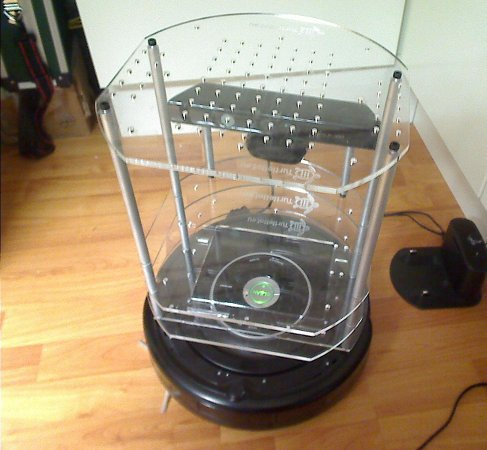
\includegraphics[width=\textwidth/3]{turtlebot.jpg}
  \caption{Turtlebot EU-Version}
  \label{figure:turtlebot}
\end{center}
\end{figure}

This thesis will have a look on the data characteristics and the accuracy of the
Kinect camera and use the results to find surfaces arranged to the camera and to 
recognize different signs on them with pattern matching in the corresponding regions
in the RGB picture. The basic idea behind is to speed up the template matching 
by only searching interesting regions of the color picture, regions which are not
suitable in size can also be skipped automatically.

\chapter{Basics}

\section{Robot Operating System (ROS)}
  
\begin{figure}[htp]
	\centering
	
\includegraphics[scale=2]{ROS_LOGO.pdf}
	\caption{ROS Logo}
\end{figure} 

The Robot Operating System or ROS for short is a meta operating system from WillowGarage, which is designed for usage with distributed 
robot systems. It's called a meta operating system because it needs another operating system to run. It's mainly developed for Ubuntu 
(a Linux distribution) but it also supports other Operating Systems like Windows and Mac OS, but the support for them can still be considered 
as experimental. 

It also works together with a Google Android device by runnning a special software which makes the device available
as hardware extension, enabling processes on different machines to access cameras, accelerometers and the display.
The basic underlying principle of ROS is the Publisher Subscriber Pattern further called PSP, it's a pattern which 
implements the realworld behaviour of publishers and subscribers (e.g. newspaper) in software. 
The publishing house advertises and publishes its newspaper or magazine while the subscribers look at the advertisements
and subscribe to the newspaper like seen in figure \vref{figure:psp_real}.

\begin{figure}[htp]
	\centering
	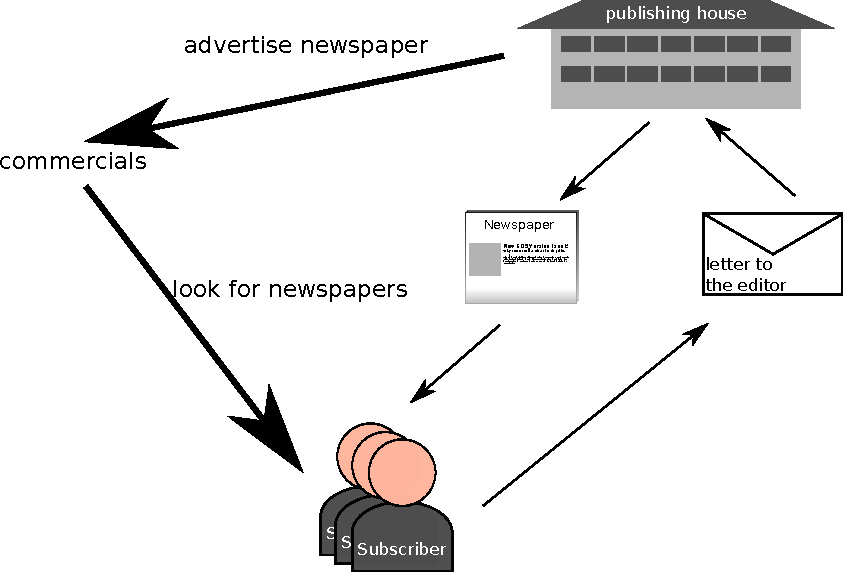
\includegraphics[scale=0.7]{PS_Newspaper.pdf}
	\caption{Publisher Subscriber Priciple in Reality}
	\label{figure:psp_real}
\end{figure} 


In the PSP the newspapers are now called topics. A PSP system is a subset of different applications, those applications are called nodes.  
Each node can publish or subscribe to multiple topics at the same time. So it is possible to create a network of different nodes, which
do processing or act as user interface. The advertisements of the real world are replaced by a so called master. 
The master knows everything about the communication channels, all nodes, the computer they run on and 
which topics they subscribe and publish to. When a new node starts up, it checks for other nodes publishing or subscribing the relevant topics
and connects with them. An example of this is shown in figure \vref{figure:psp_ROS}.
In the picture there are different nodes for the robots running gear, its laserscanner, the motion planing system and the graphical user interface.
connected together by topics.

\begin{figure}[htp]
	\centering
	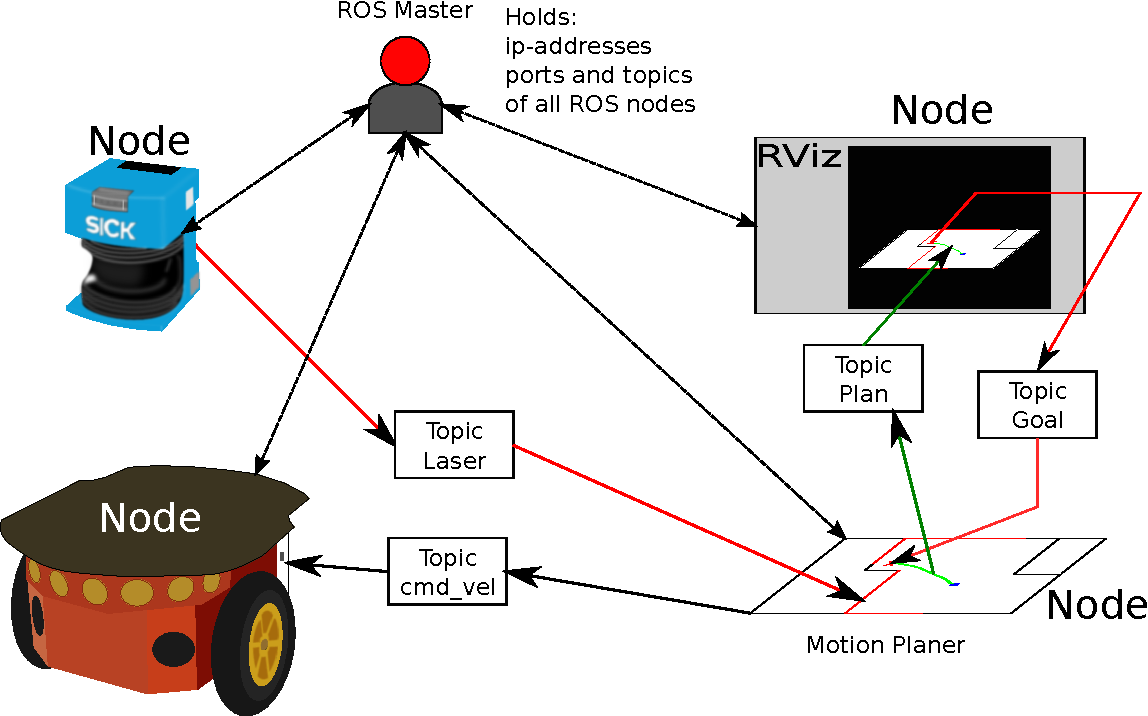
\includegraphics[scale=0.6]{PS_ROS.pdf}
	\caption{Publisher Subscriber Pattern in ROS}
	\label{figure:psp_ROS}
\end{figure} 

In this work the output of the rViz-node (short form for robot visualizer) will be used to display changes to the depth- and 
rgb-image of the Kinect. rViz is a tool to display various informations like video streams, maps, paths, positions and the
so called point cloud.
\clearpage

\section{Point Cloud}
The point cloud is data set which contains the three dimensional position for each pixel of a 3D camera. 
If available, it can also contain the color or grayscale values of each pixel. 
The point cloud data can be collected from a stereo camera, a laser scanner which rotates around an axis or 
from cameras like the Microsoft Kinect.

\begin{figure}[htp]
	\centering
	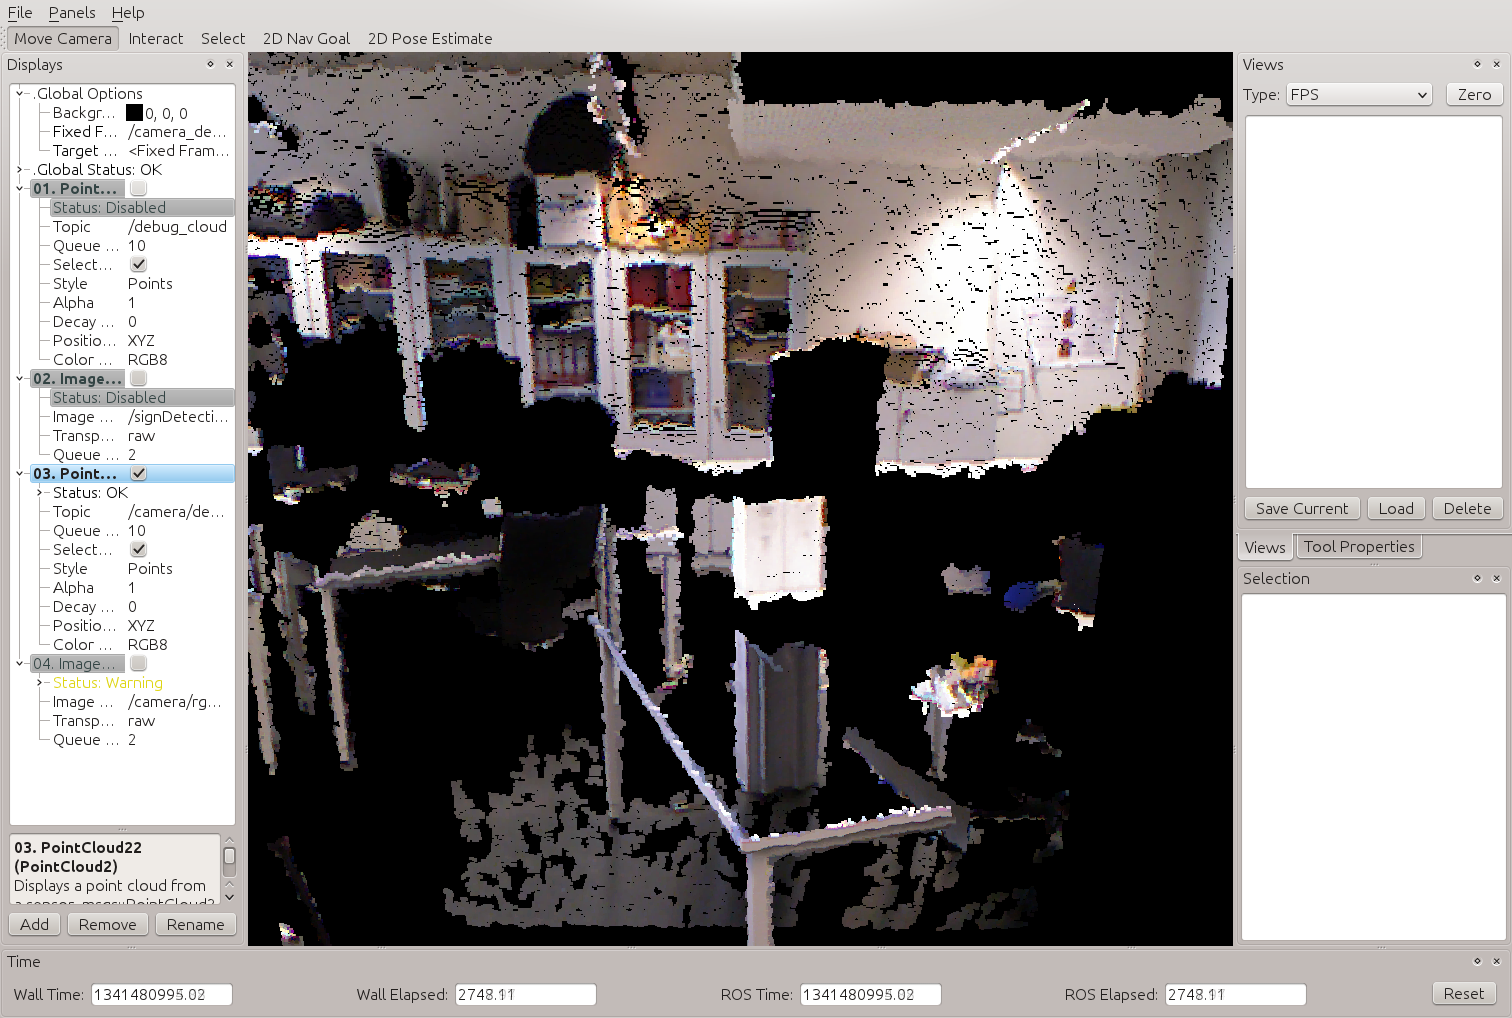
\includegraphics[width=\textwidth]{RVizPointCloud.png}
	\caption{Robot Visualizer displaying the Point Cloud}
	\label{figure:RVizPointCloud.png}
\end{figure}
\clearpage

\section[OpenCV]{OpenCV \footnote{Text for this section was taken from manufacturer website \url{http://opencv.org/about.html}\cite{willowgarage:opencv}}}

The Open Source Computer Vision Library (OpenCV) is an open computer vision and machine learning software library. OpenCV was built to provide a common infrastructure for vision applications and to accelerate the use of machine perception in the commercial products. To enable this, OpenCV has a BSD license to make it easy for businesses to use and modify the code.

The library has more than 2500 optimized algorithms. OpenCV contains a comprehensive set of both classic and state of the art computer vision and machine learning algorithms. These algorithms can be used, for example, to detect and recognize faces, identify objects, classify human actions in videos, track camera movements, track moving objects, extract 3D models of objects, produce 3D point clouds from stereo cameras, stitch images together to produce a high resolution image of an entire scene, find similar images from an image database, remove red eye from images taken using flash, follow eye movements, recognize scenes and establish markers to overlay the scenes with augmented reality to name a few. OpenCV has well over 5 million downloads, has an active user group with over 47 thousands registered members. OpenCV is used extensively in companies, research groups and by governmental bodies.

Some well known companies that use OpenCV are Google, Yahoo, Microsoft, Intel, IBM, Sony, Honda, Toyota. Many startups such as Applied Minds, VideoSurf, and Zeitera make extensive use of OpenCV. OpenCV’s deployed uses span the range from stitching streetview images together, detecting intrusions in surveillance video in Israel, monitoring mine equipment in China, helping robots navigate and pick up objects at Willow Garage, detection swimming pool drowning events in Europe, running interactive art in Spain and New York, checking run ways for derbies in Turkey, inspecting labels on products in factories around the world on to rapid face detection in Japan.

It runs on Windows, Linux, Mac, Android and has C++, C, Python and Java (Android only) interfaces. OpenCV leans mostly towards real-time vision applications and takes advantage of MMX and SSE instructions when available. A CUDA interface is being developed right now. There are over 500 algorithms and about 10 times as many functions that compose or support those algorithms. OpenCV is written natively in C++ and has a templated interface that works seamlessly with std containers. Its native data type is a general matrix class that reference counts and leverages EIGEN.
\clearpage

\section{Kinect}
\begin{figure}[htp]
	\centering
	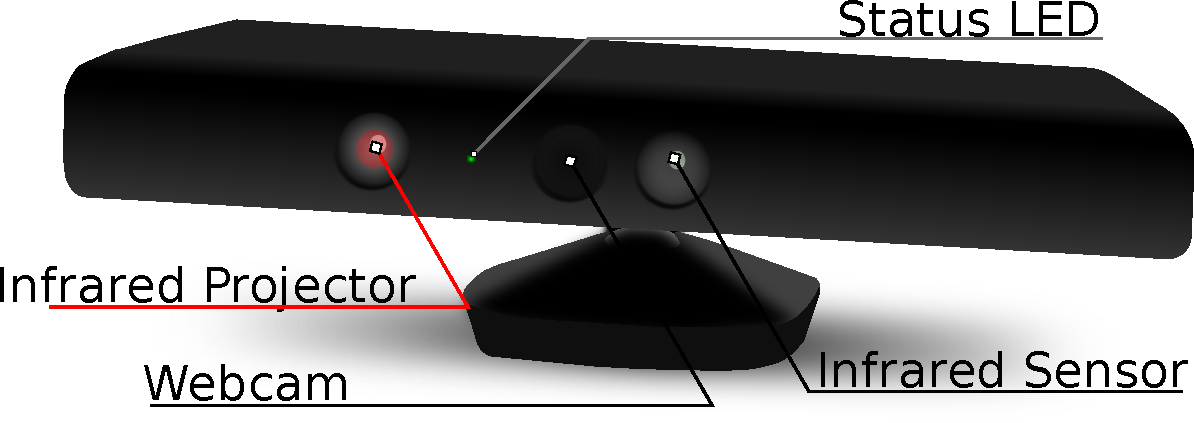
\includegraphics[scale=0.7]{Kinect.pdf}
	\caption{Microsoft Kinect Camera Overview}
	\label{figure:kinect_camera}
\end{figure}

The Kinect is a combination of a standard color camera and a depth sensor produced by Microsoft, a so called RGB-D camera. 
The depth sensor is produced by Primesense and its working principle is currently a secret of the manufacturer. 
The known facts are, that the Kinect uses an ir-projector to draw a grid of very small points onto each surface 
(see figure \vref{figure:kinect_camera}) and an IR-camera to process the result somehow.  
There are different approaches on how it might work, the most resonable approach is that it uses 
specific groups of points and their position on the resulting camera image to calculate how far 
away they are. This is the same way a laser scanner works. 
It sends out a laser beam and the sensor is aranged in a different viewing angle than the beam.
If the beam now hits a surface its position in the camera picture relates to the distance of the surface.
(see in figure \vref{figure:ls_WP}). This it would be the same for the Kinect points but in 3 dimensions 
(see in figure \vref{figure:kinect_WP}).

ASUS is also offering cameras with the Primesense chipset for developers, the XTion Pro and the XTion Pro Live.
The difference between those cameras is, that the XTion Pro does not include a webcam.

In the recent past Microsoft created a new PC version of the Kinect, which is called Kinect for Windows.
This camera offers a greater viewing angle, while being able to detect objects closer to the camera.
The problem of objects being to close will be discussed later in this document.

\begin{figure}[htp]
	\centering
	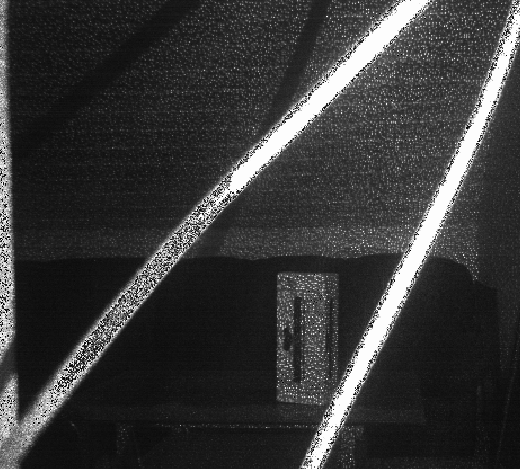
\includegraphics[scale=1]{ir_kinect.png}
	\caption{Kinect IR Sensor Image making IR Spots visible)}
	\label{figure:kinect_ir}
\end{figure}

\begin{figure}[htp]
	\centering
	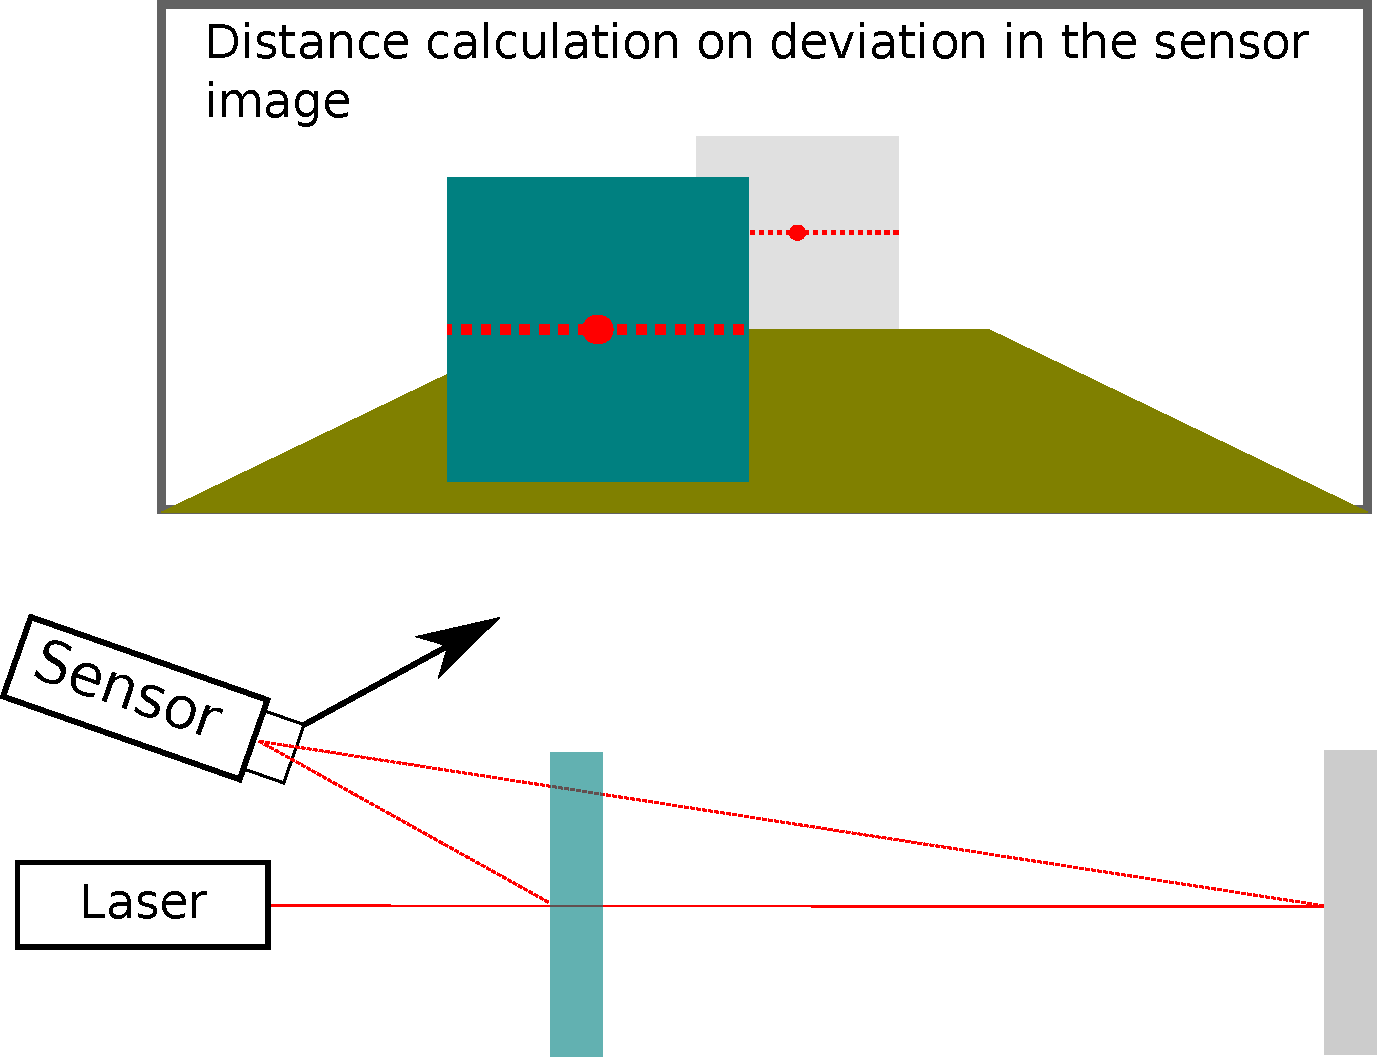
\includegraphics[scale=0.5]{laserScannerPrinciple.pdf}
	\caption{Laser Scanner Working Principle}
	\label{figure:ls_WP}
\end{figure}


\begin{figure}[htp]
	\centering
	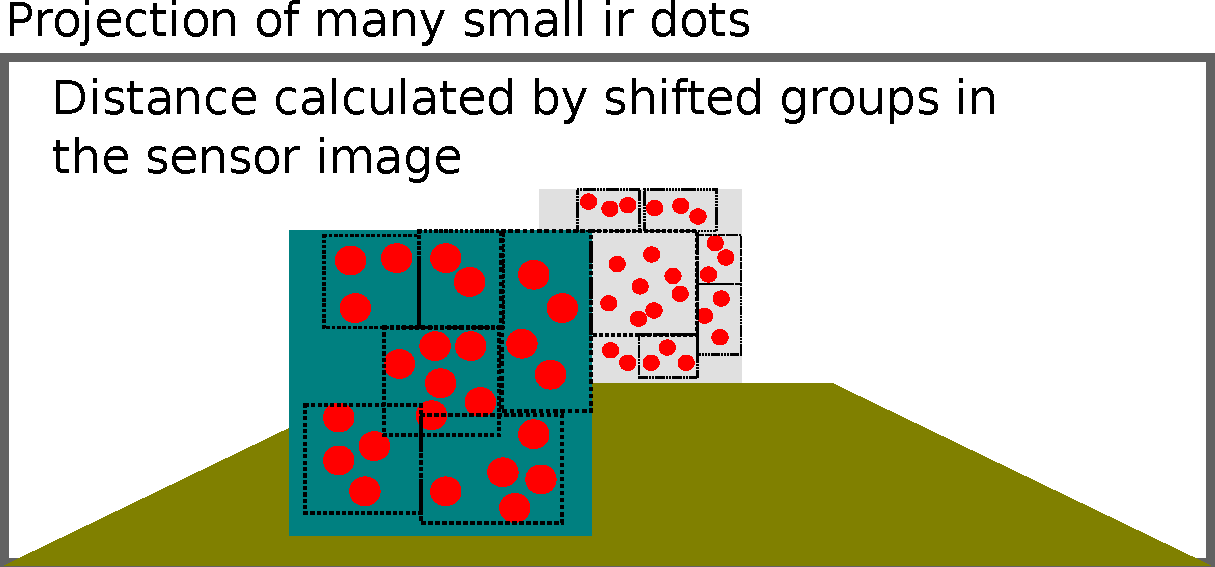
\includegraphics[scale=0.5]{kinect_principle.pdf}
	\caption{Kinect Working Principle}
	\label{figure:kinect_WP} 
\end{figure}
\clearpage

\section[OpenNi]{OpenNi \footnote{Text for this section was taken from organisation website \url{http://www.openni.org/About.aspx} \cite{openni:about}}}

About the OpenNI organization
The OpenNI organization is an industry-led, not-for-profit organization formed to certify and 
promote the compatibility and interoperability of Natural Interaction devices, applications and middleware. 
One of the OpenNI organization goals is to accelerate the introduction of Natural Interaction applications into 
the marketplace.

The founding members of the OpenNI organization are:
\begin{itemize}
  \item PrimeSense, industry leader in Natural Interaction and 3D depth sensing solutions   
  \item Willow Garage, experts in personal robotics applications  
  \item Side-Kick, a leading production house for motion control games  
  \item ASUS joins the OpenNI organization as an industry member providing hardware for purchase to promote Natural Interaction applications
  \item AppSide is the first end-to-end content marketplace for motion-controlled entertainment devices. 
\end{itemize}

\section{Mobile Robots Pioneer 3dx}
The Pioneer 3dx is a Research Robot created by Mobile Robots.
\\
\url{http://www.mobilerobots.com/ResearchRobots/PioneerP3DX.aspx}
\\
With its two motored wheels and its stabilization wheel the robot is a so called point robot. That means it's able to 
rotate around its center like a tank which makes path planing and movement a lot easier. 
The robot features a internal microcontroller board which can be remote controlled from an external computing system, 
ultra-sonic distance sensors and bumpers. The robot of the University of Applied Sciences Aalen 
is additionally equipped with a LMS-200 laser scanner from SICK Sensor Technologies, which works
like described in the last chapter.


\begin{figure}[htp]
\begin{center}
  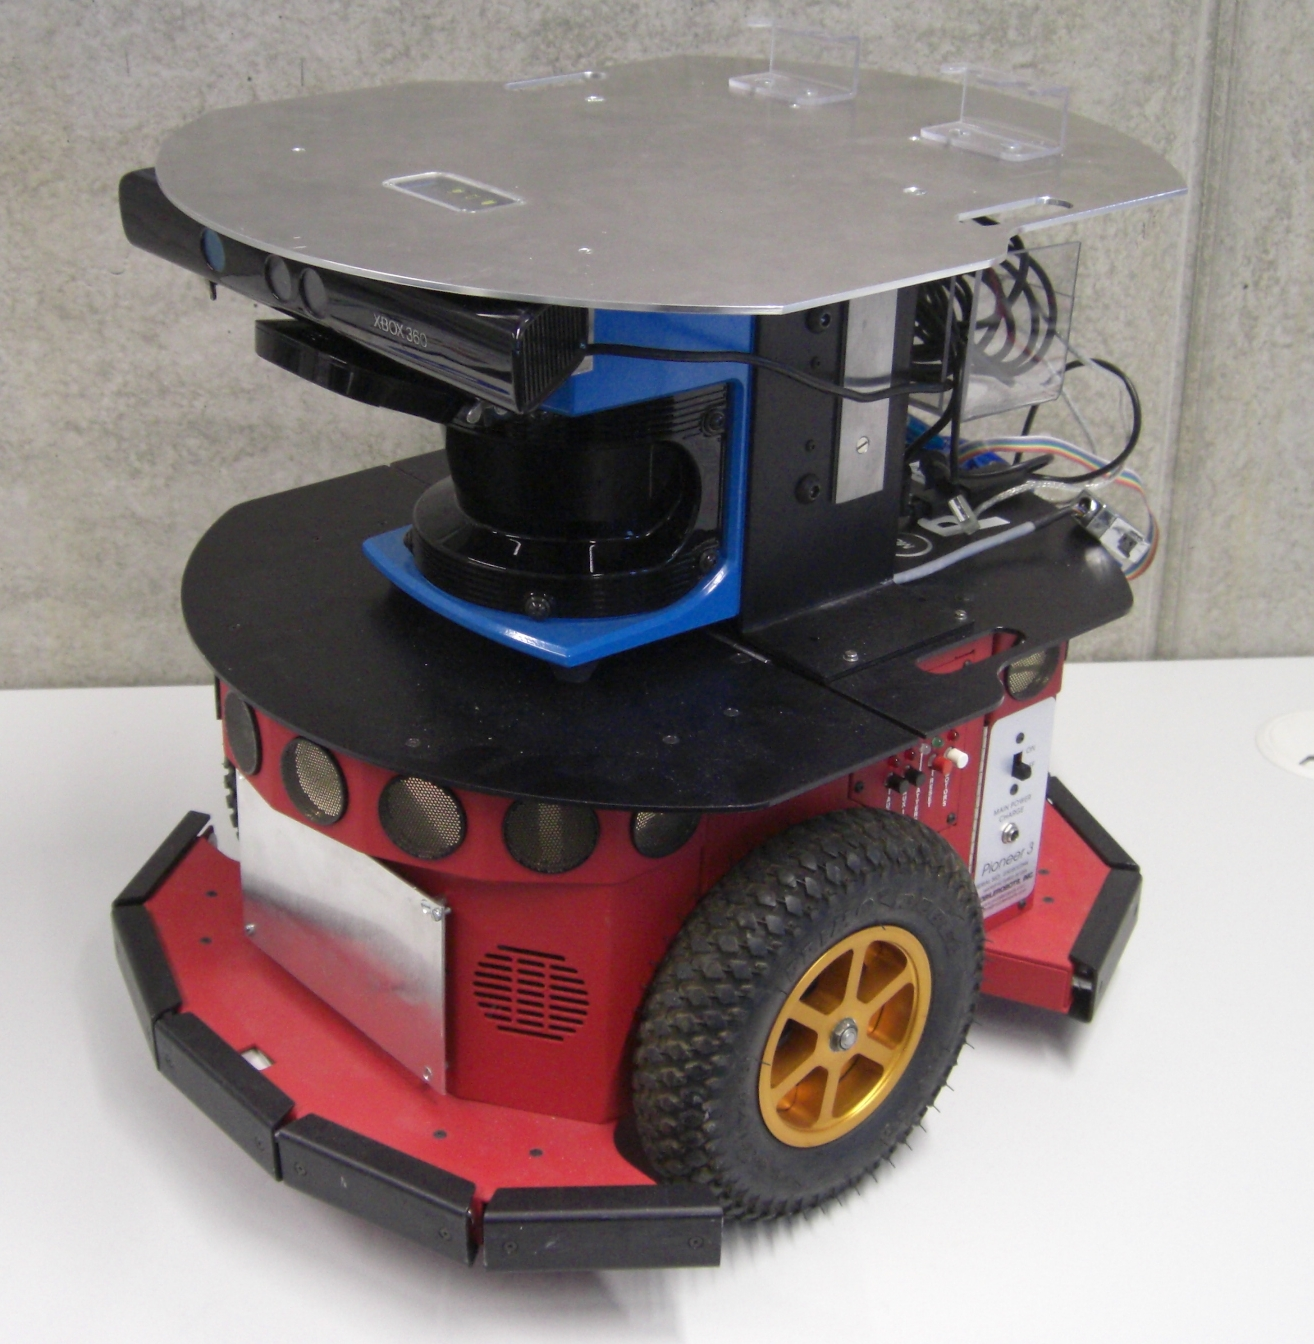
\includegraphics[height=\textheight/3]{pioneer.JPG}
  \caption{Pioneer 3DX}
  \label{figure:Pioneer}
\end{center}
\end{figure}




 

 

\chapter{Mechanical Parts}
\graphicspath{{./Mechanical/img/}}



\section{Signs}

For the signs, which have to be recognized by the software, sign posts (see in figure \vref{figure:signs}) where created.
They consist of a round plate with a thread on the side, a round stand with a thread in the middle and a staff connecting
with a thread on each side to connect them.

The diameter of the sign is 15 cm and it's overall height measures 50 cm.

The signs graphic, a standardized european speed limit sign, was taken from 
Wikipedia\footnote{\url{http://upload.wikimedia.org/wikipedia/commons/archive/2/2e/20120617230605!Zeichen_274-56.svg}}
and modified to have an arrow in it's center. 

 \begin{figure}[htp]
\begin{center}
  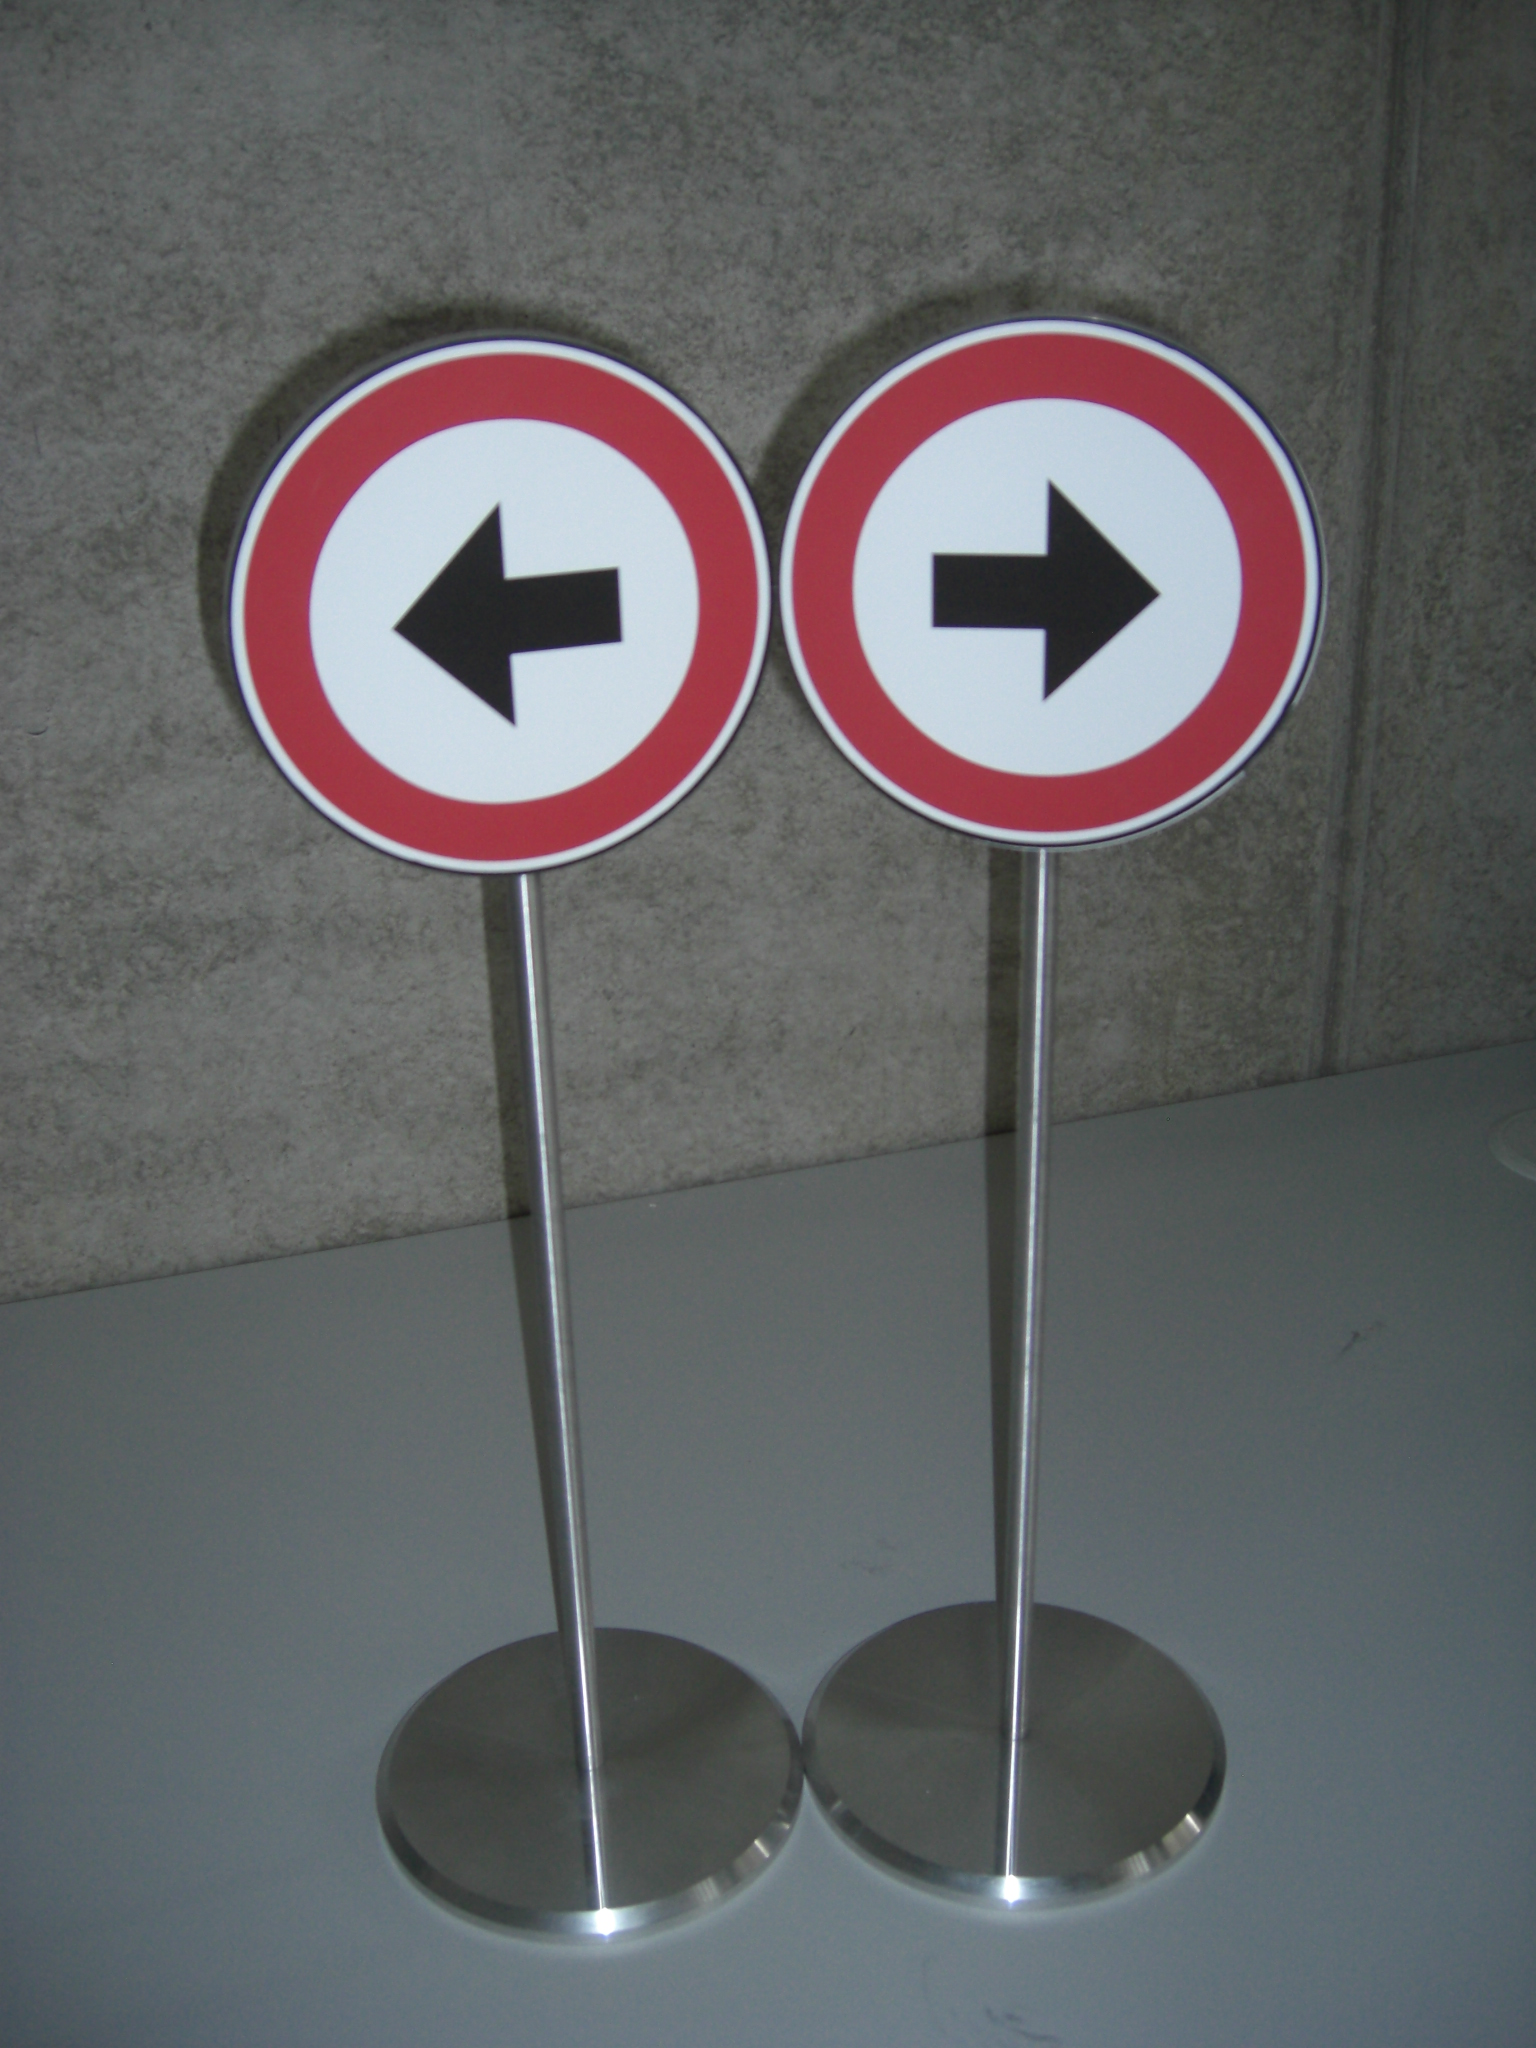
\includegraphics[width=\textwidth/3]{signs.jpg}
  \caption{Signs for Recognition}
  \label{figure:signs}
\end{center}
\end{figure}

\section{Robot Update}

For using the Kinect with the given Pioneer 3dx it was necessary to fix the camera at the robot.
Due to some lacks of the previous laptop stand, it was decided to completely rework it.

The old laptop stand as seen in figure \vref{figure:old_stand}, had problems with rust and weight,
because it is made of steel. Another disadvantage is, that the Laptop bracket, which keeps the 
controlling laptop from tilting, is made out of aluminium and has sharp corners. This can lead
to a damage of the laptops case, especially when the laptop is removed from the stand. 

\begin{figure}[htp]
\begin{center}
  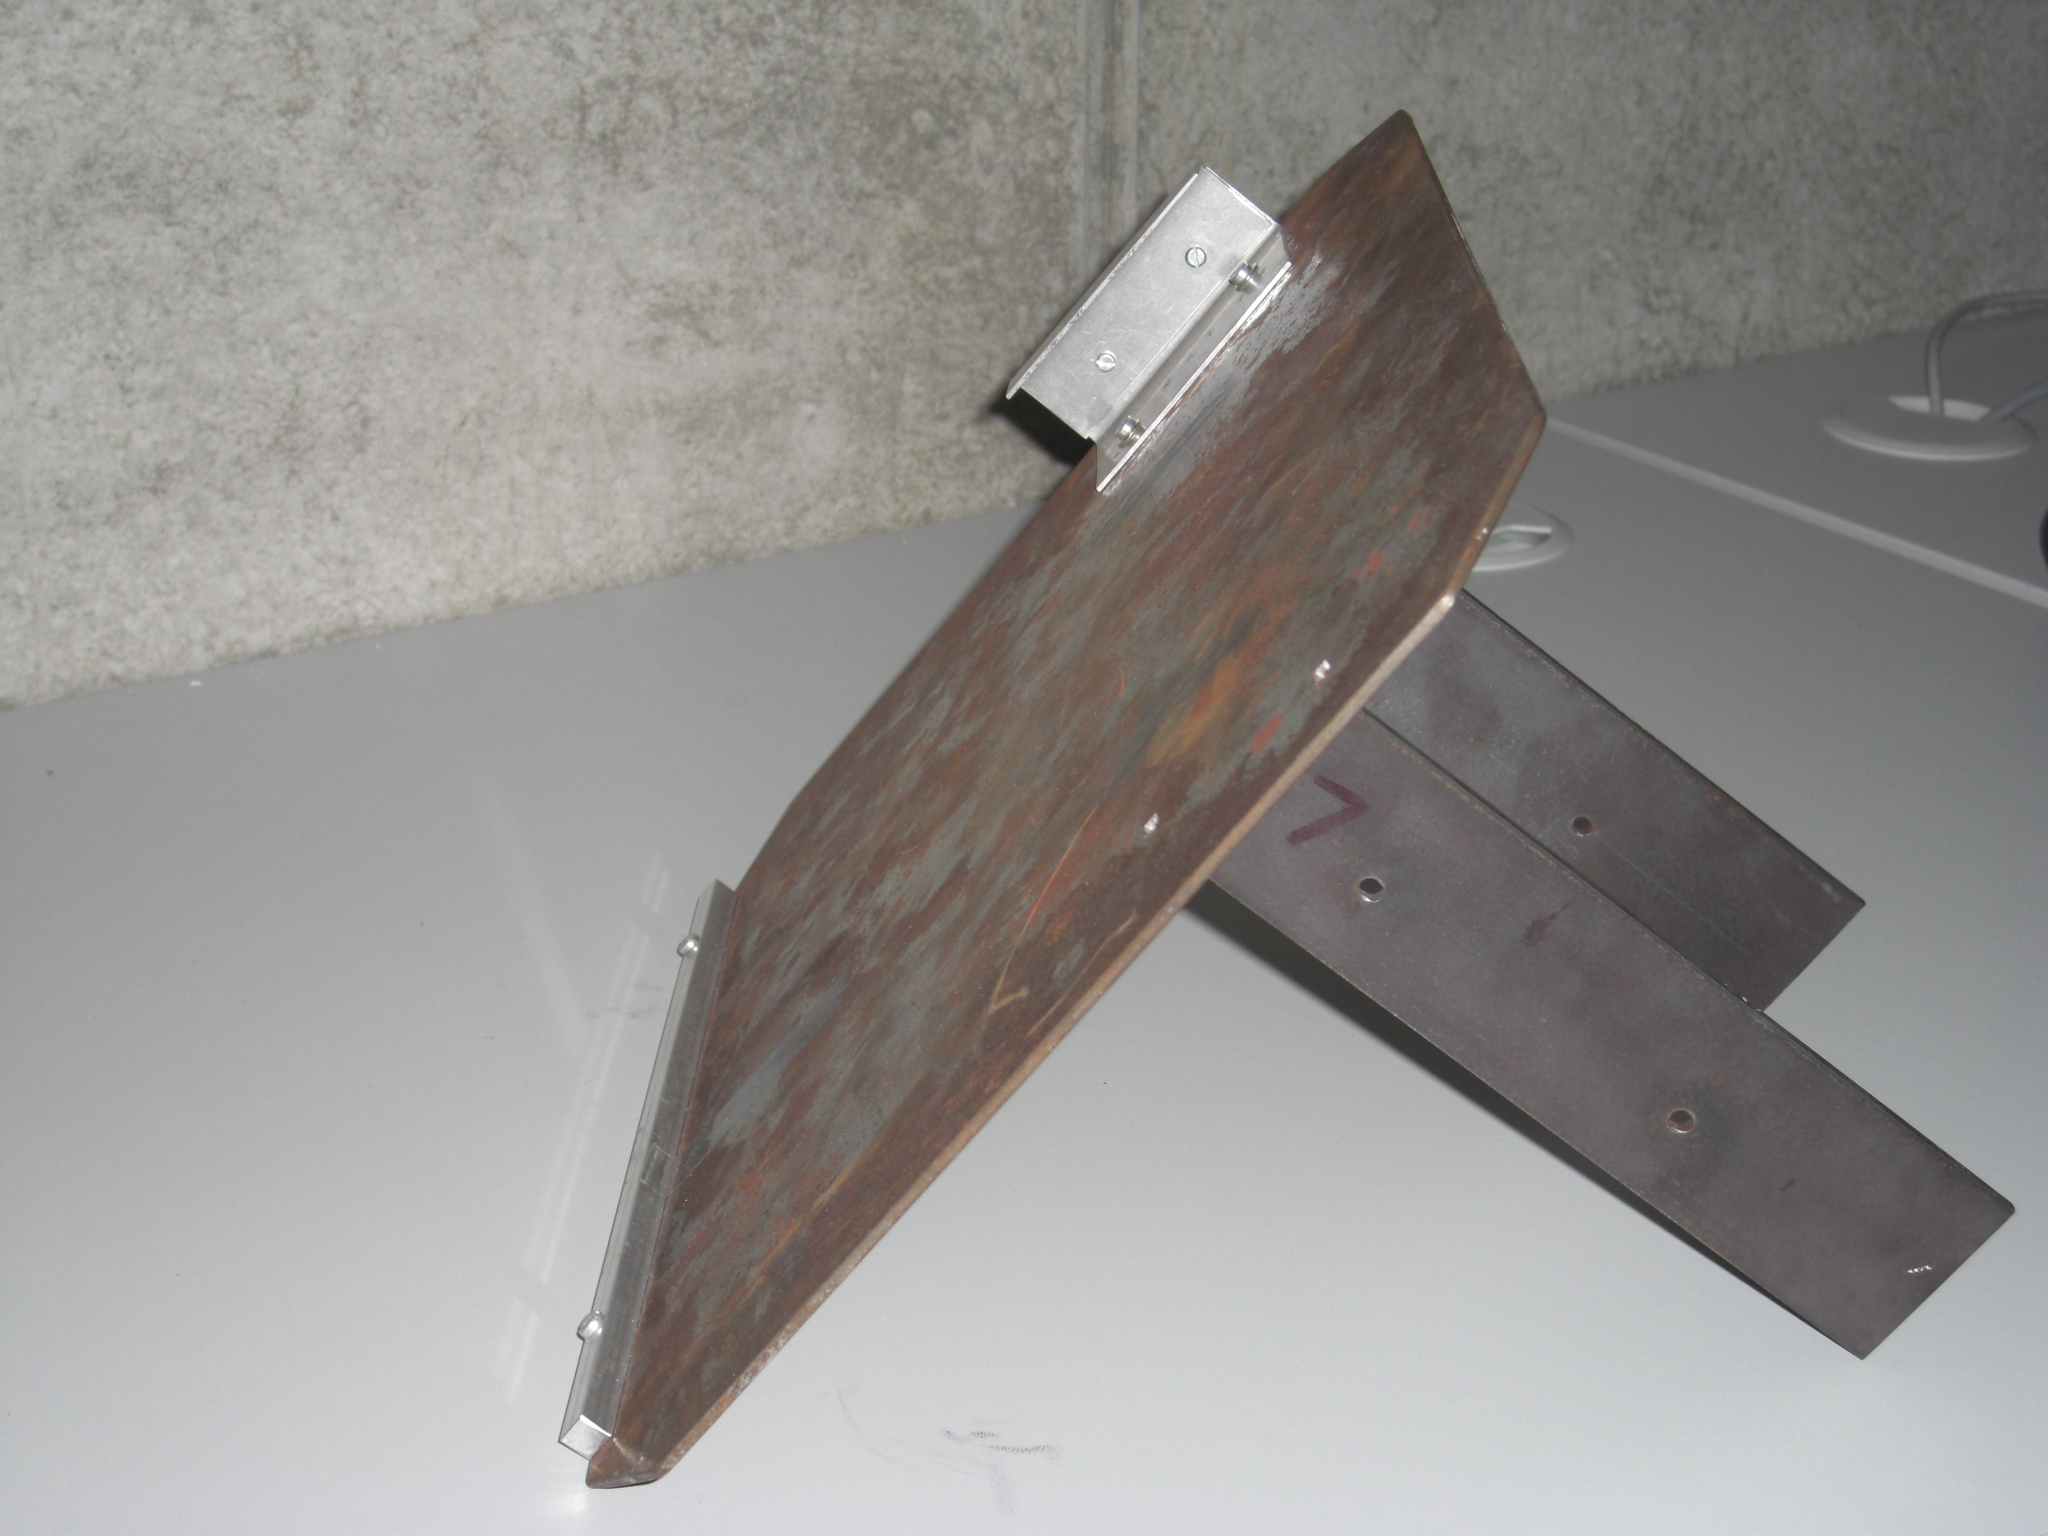
\includegraphics[width=\textwidth/2]{old_laptop_stand.jpg}
  \caption{Old Laptop Stand}
  \label{figure:old_stand}
\end{center}
\end{figure}


The new stand as seen in figure \vref{figure:laptop_stand} and \vref{figure:laptop_stand_side} is now lower at
weight and doesn't rust because the main tray is made out of aluminium. The new laptop brackets 
(see in figure \vref{figure:laptop_bracket}) are made out acrylic glas and have rounded down edges and corners, 
so it's mostly impossible to damage the laptops casing. The stand also features a Kinect holder 
(see in figure \vref{figure:kc_hold}) from where the Kinect can be easily dismounted. For dismounting, 
it is only necessary to loosen two wing nuts. A possible disadvantage of the new design, a bad visibility of
the status LEDs of the laser scanner, could be detected within the design process. 
To avoid this design flaw, a viewing window was constructed into the tray (see in figure \vref{figure:viewingwindow}). 
If using a 15" laptop for controlling the robot, the viewing window is completely uncovered 
(see in figure \vref{figure:viewingwindowlaptop}). Normally a newer netbook can be considered to be 
adequate in performance to control the robot. Another feature is the invented cable box 
(shown in figure \vref{figure:laptop_stand_side}), which helds the very long cable of the Kinect camera. 
Additionally the form of the main tray fits the form of the robots tray, making it look like in a more professional 
way and also like done by the manufacturer. The only thing to improve this would be, to paint the tray in the 
same dark grey color which is used for the robots tray.

\begin{figure}[htp]
\begin{center}
  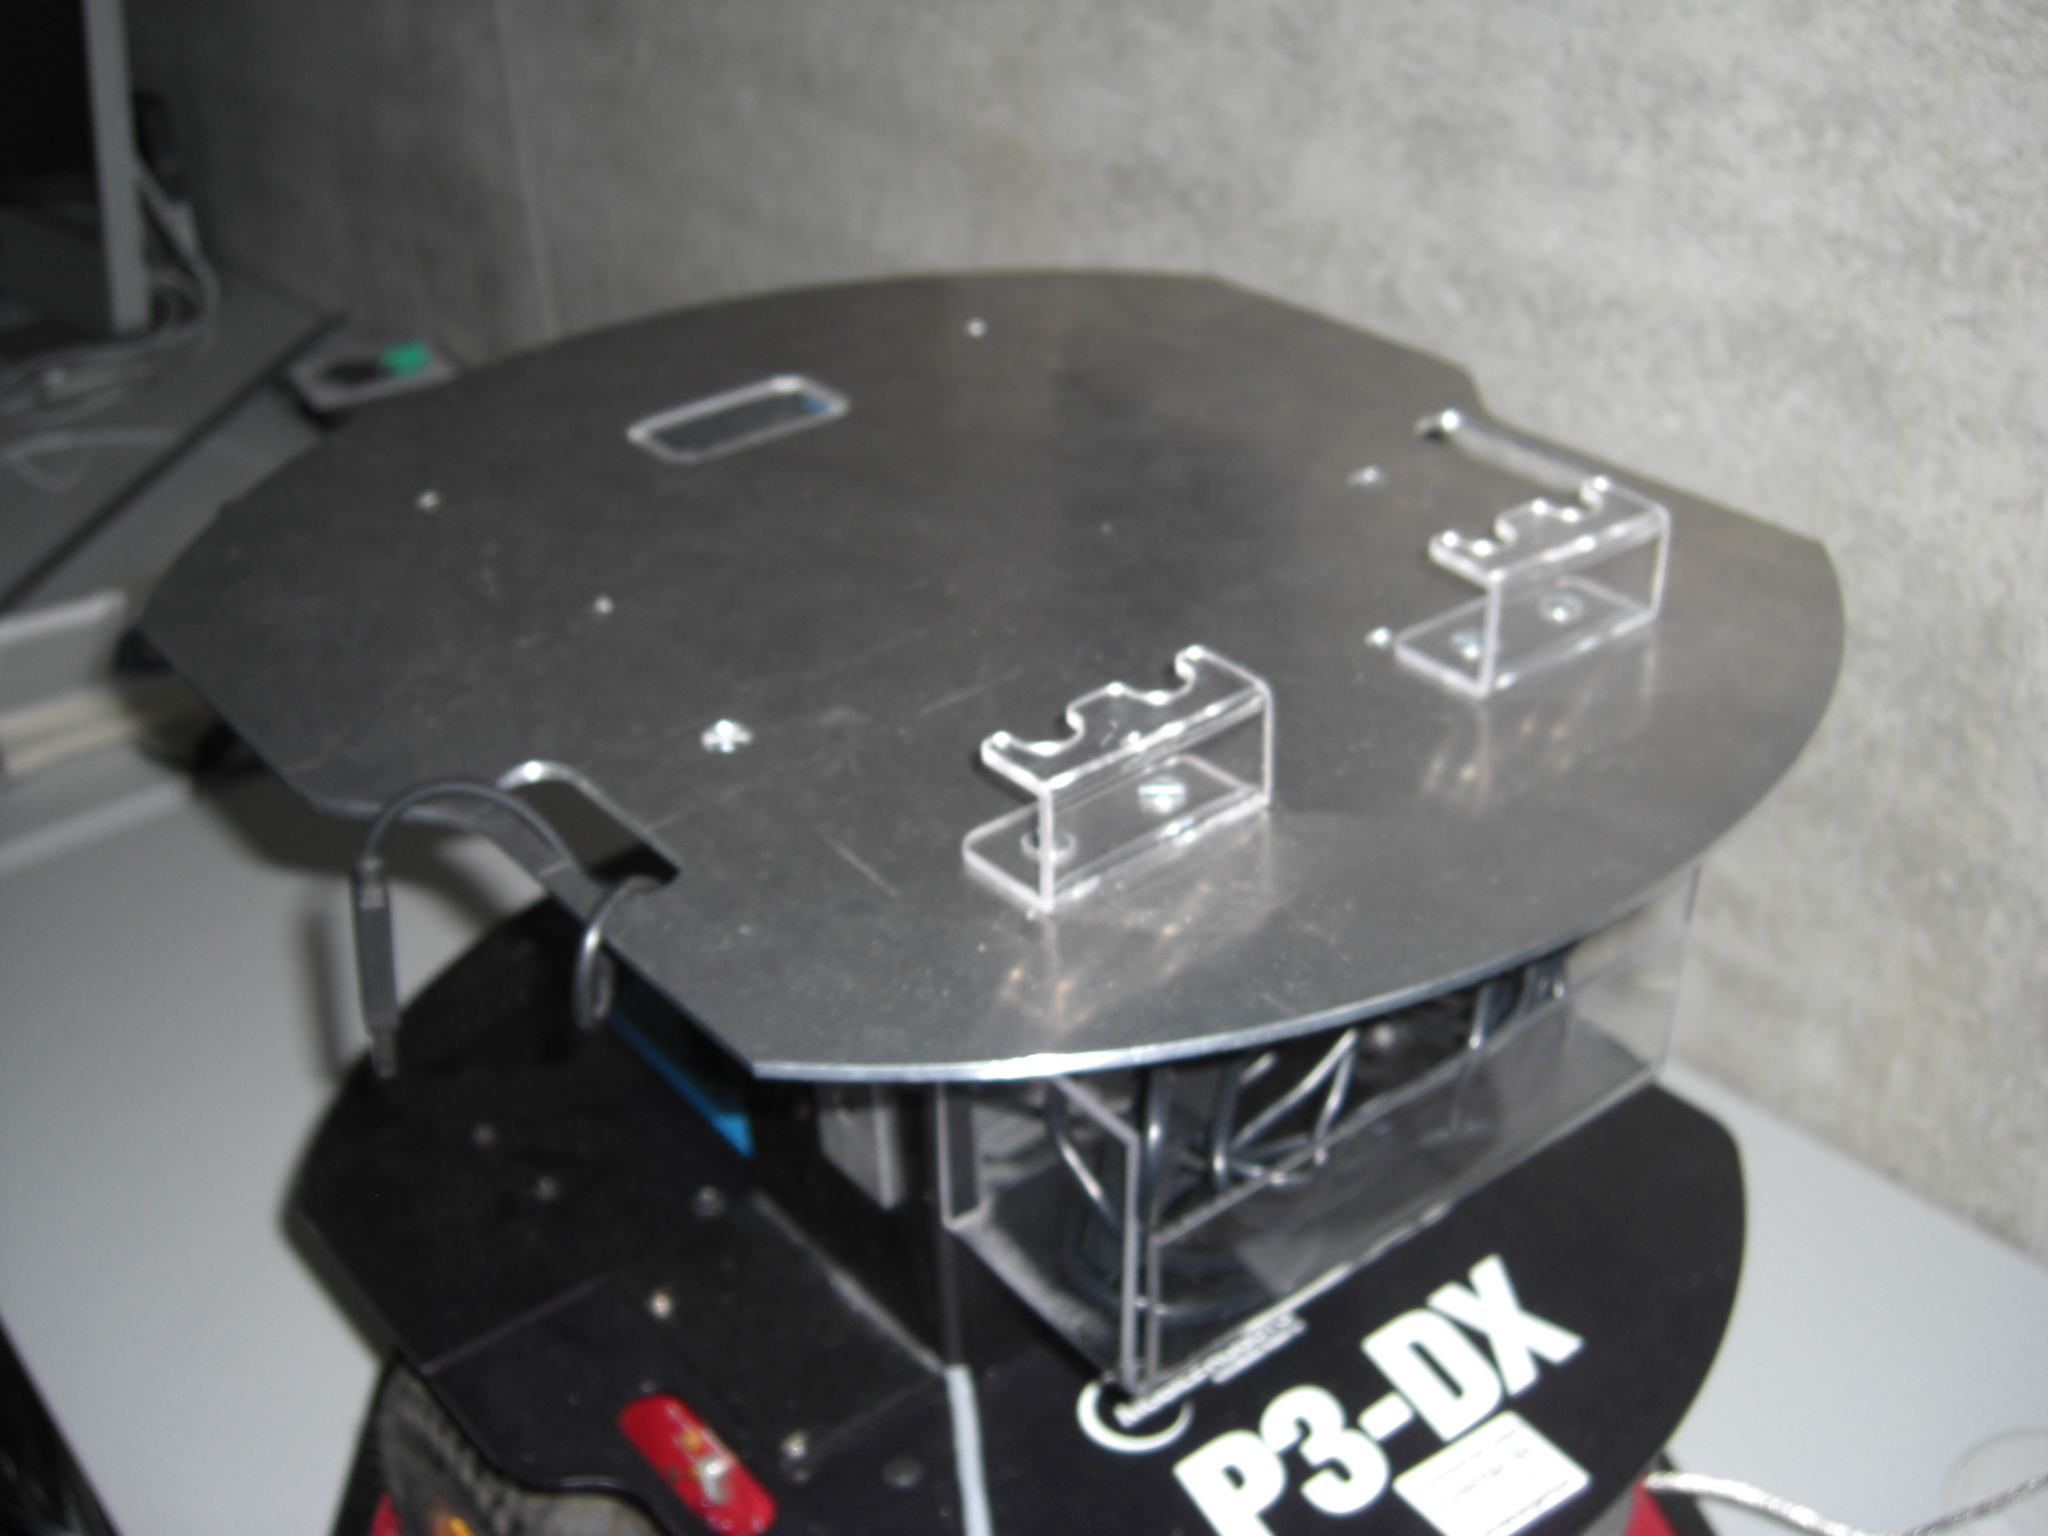
\includegraphics[width=\textwidth/2]{laptop_stand.jpg}
  \caption{Laptop Stand}
  \label{figure:laptop_stand}
\end{center}
\end{figure}
\begin{figure}[htp]
\begin{center}
  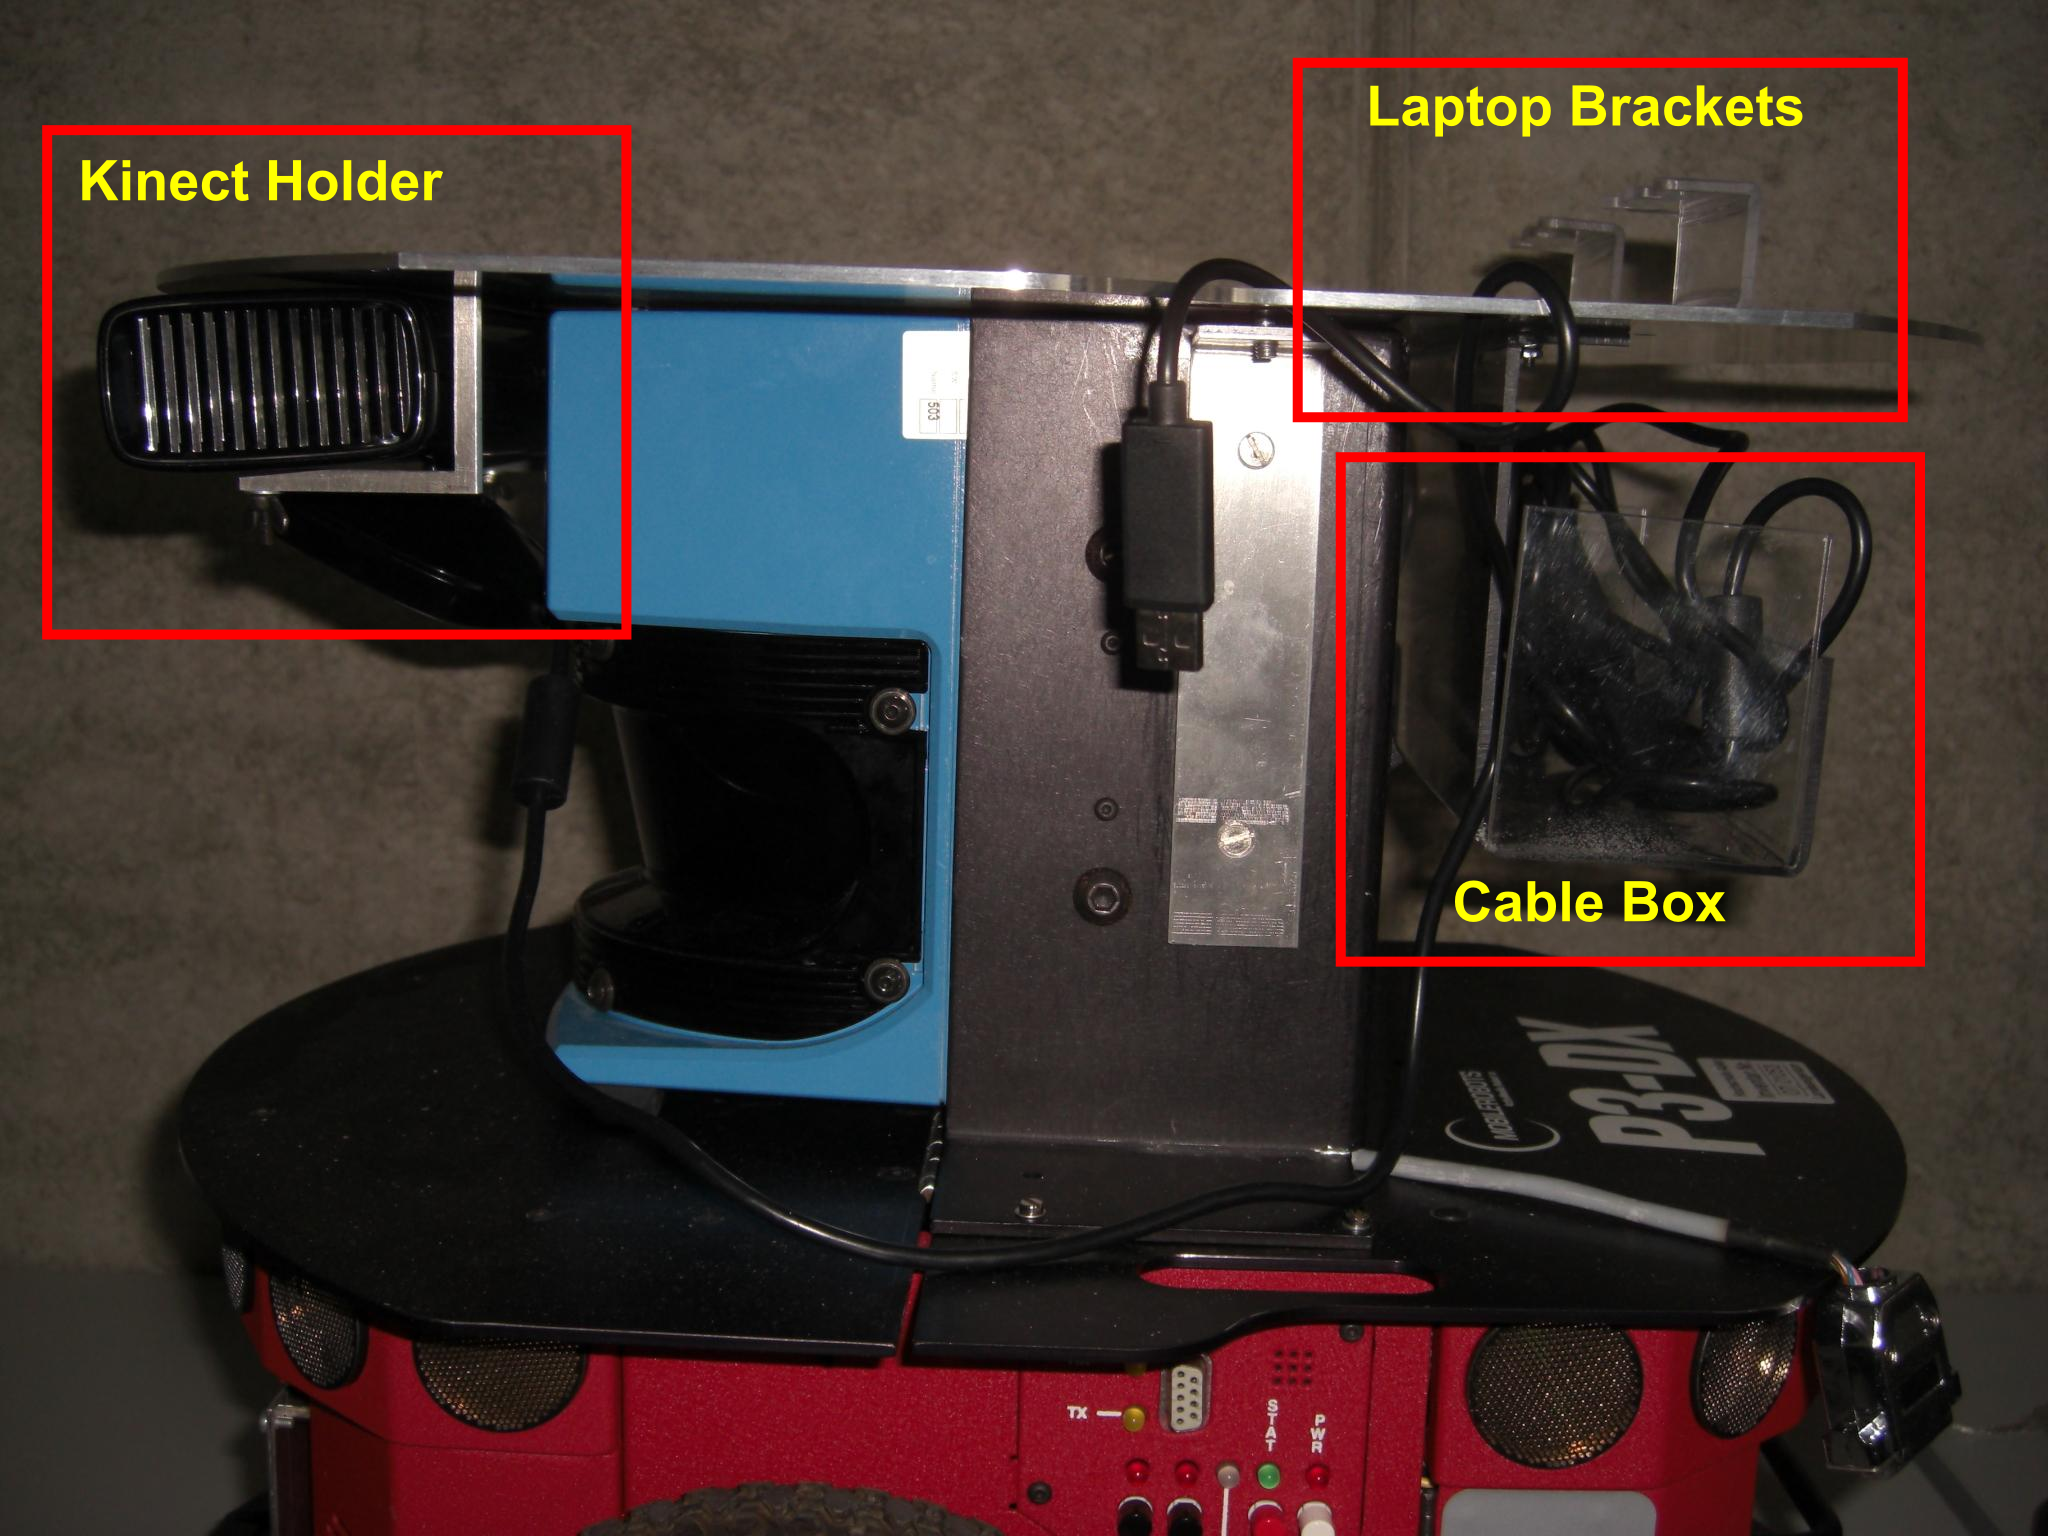
\includegraphics[width=\textwidth]{laptop_stand_side.png}
  \caption{Laptop Stand Feature Overview}
  \label{figure:laptop_stand_side}
\end{center}
\end{figure}


\begin{figure}[htp]
\begin{center}
  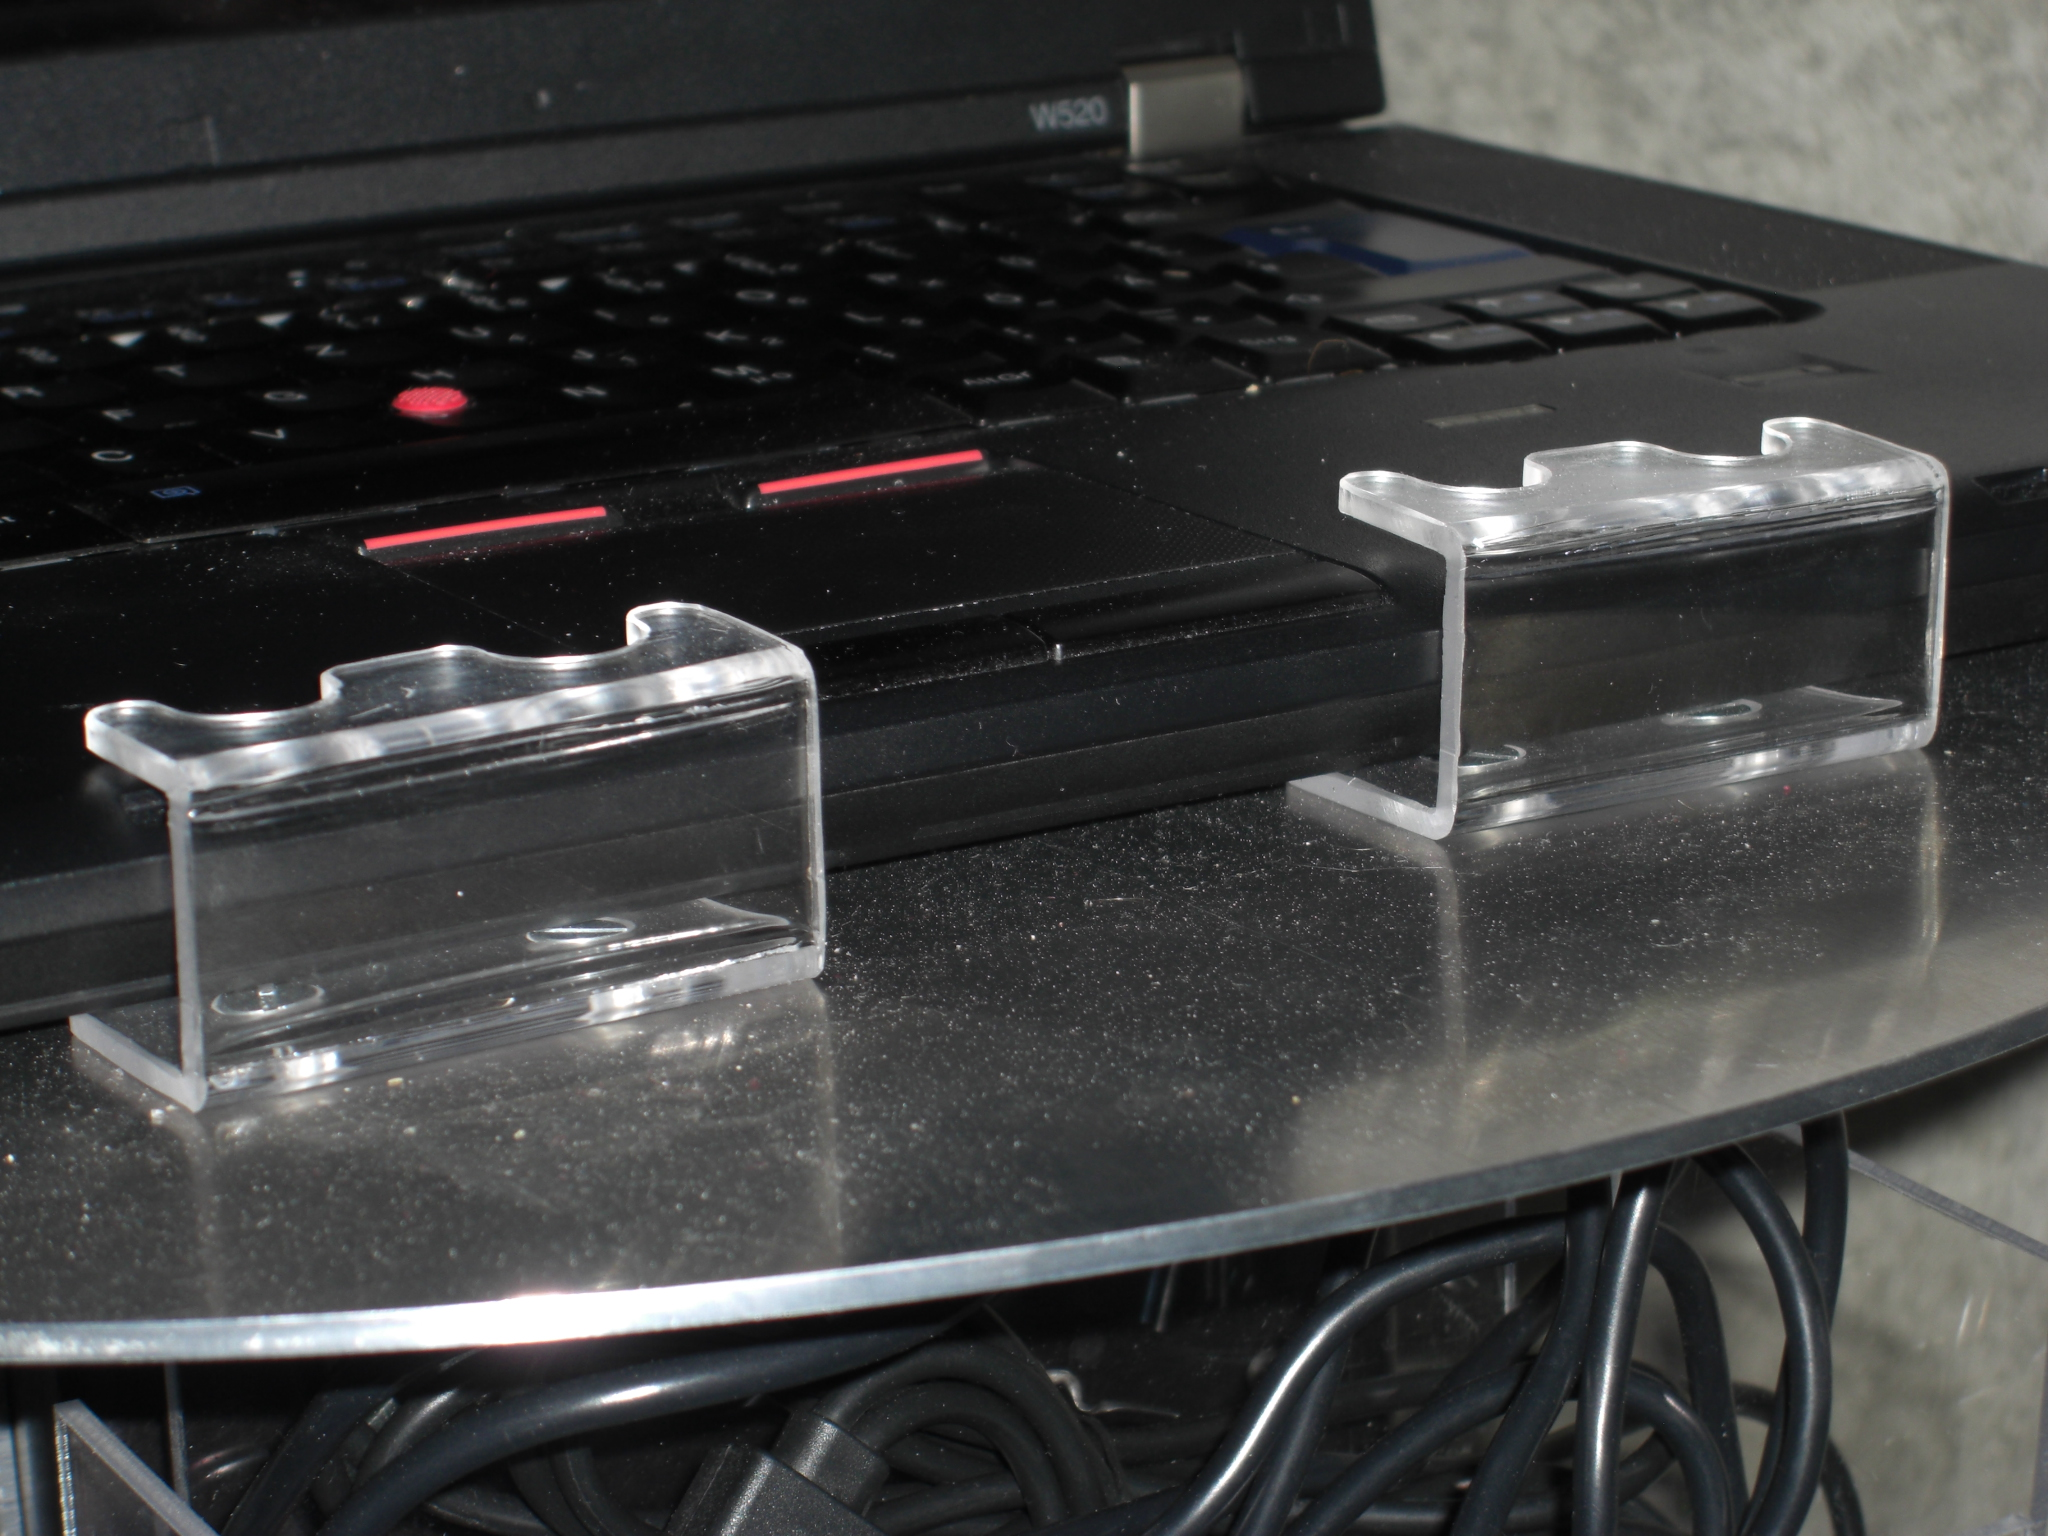
\includegraphics[width=\textwidth/2]{laptop_bracket.jpg}
  \caption{Holding Brackets for Laptops}
  \label{figure:laptop_bracket}
\end{center}
\end{figure}
\begin{figure}[htp]
\begin{center}
  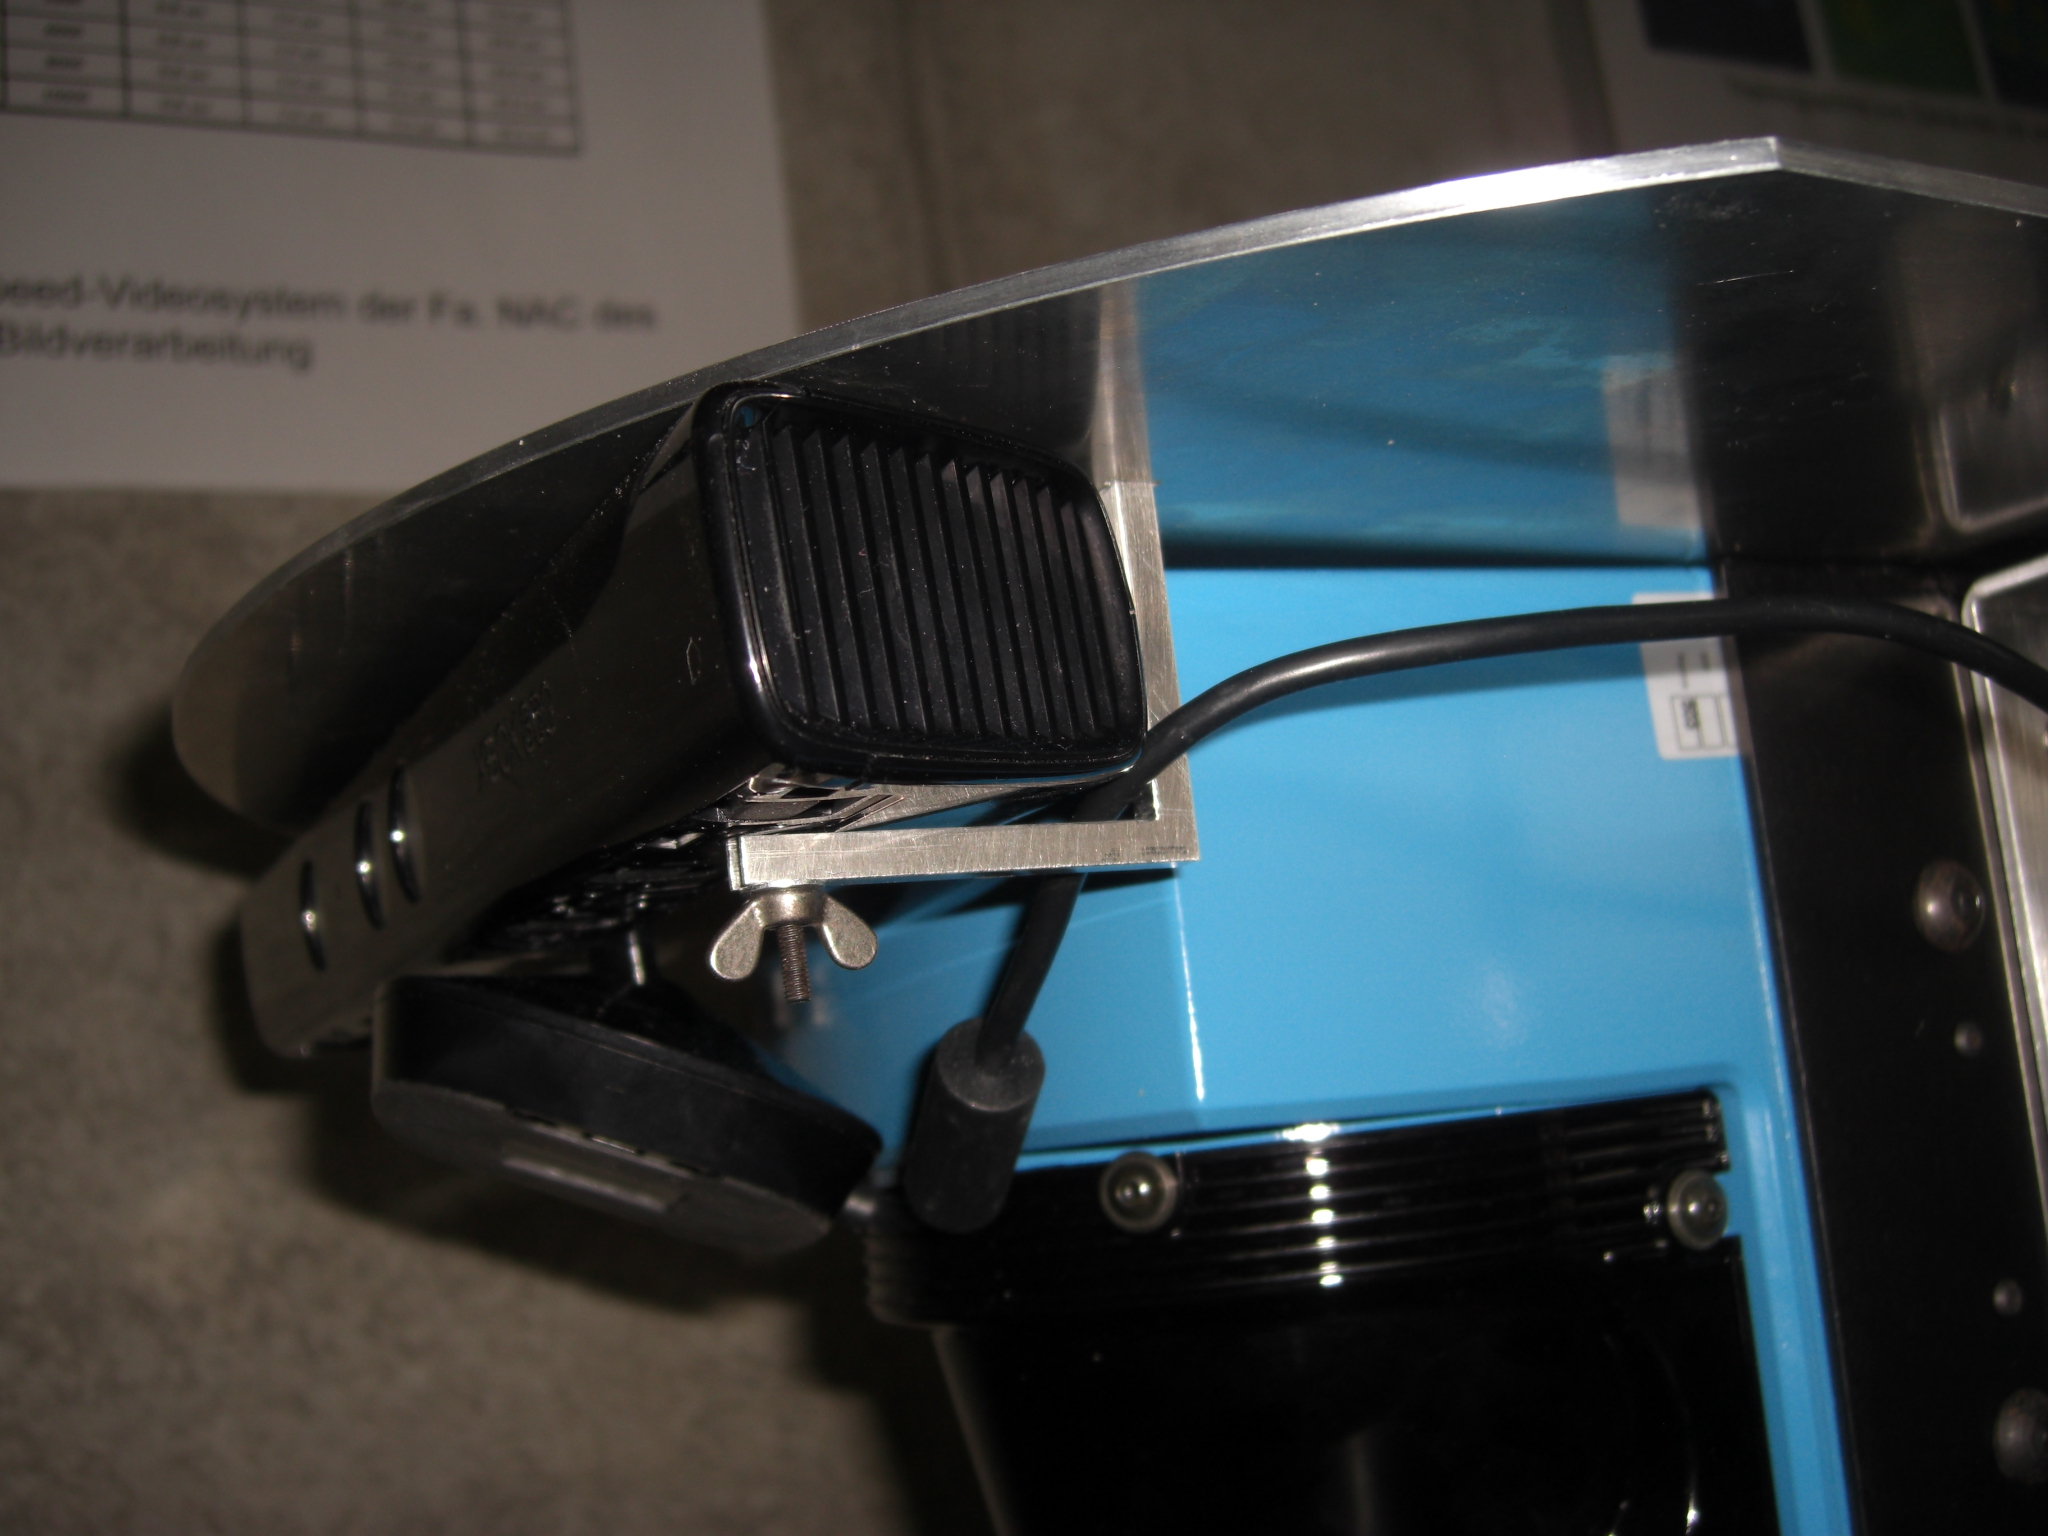
\includegraphics[width=\textwidth]{kinect_bracket.jpg}
  \caption{Kinect Camera Holder}
  \label{figure:kc_hold}
\end{center}
\end{figure}

\begin{figure}[htp]
\begin{center}
  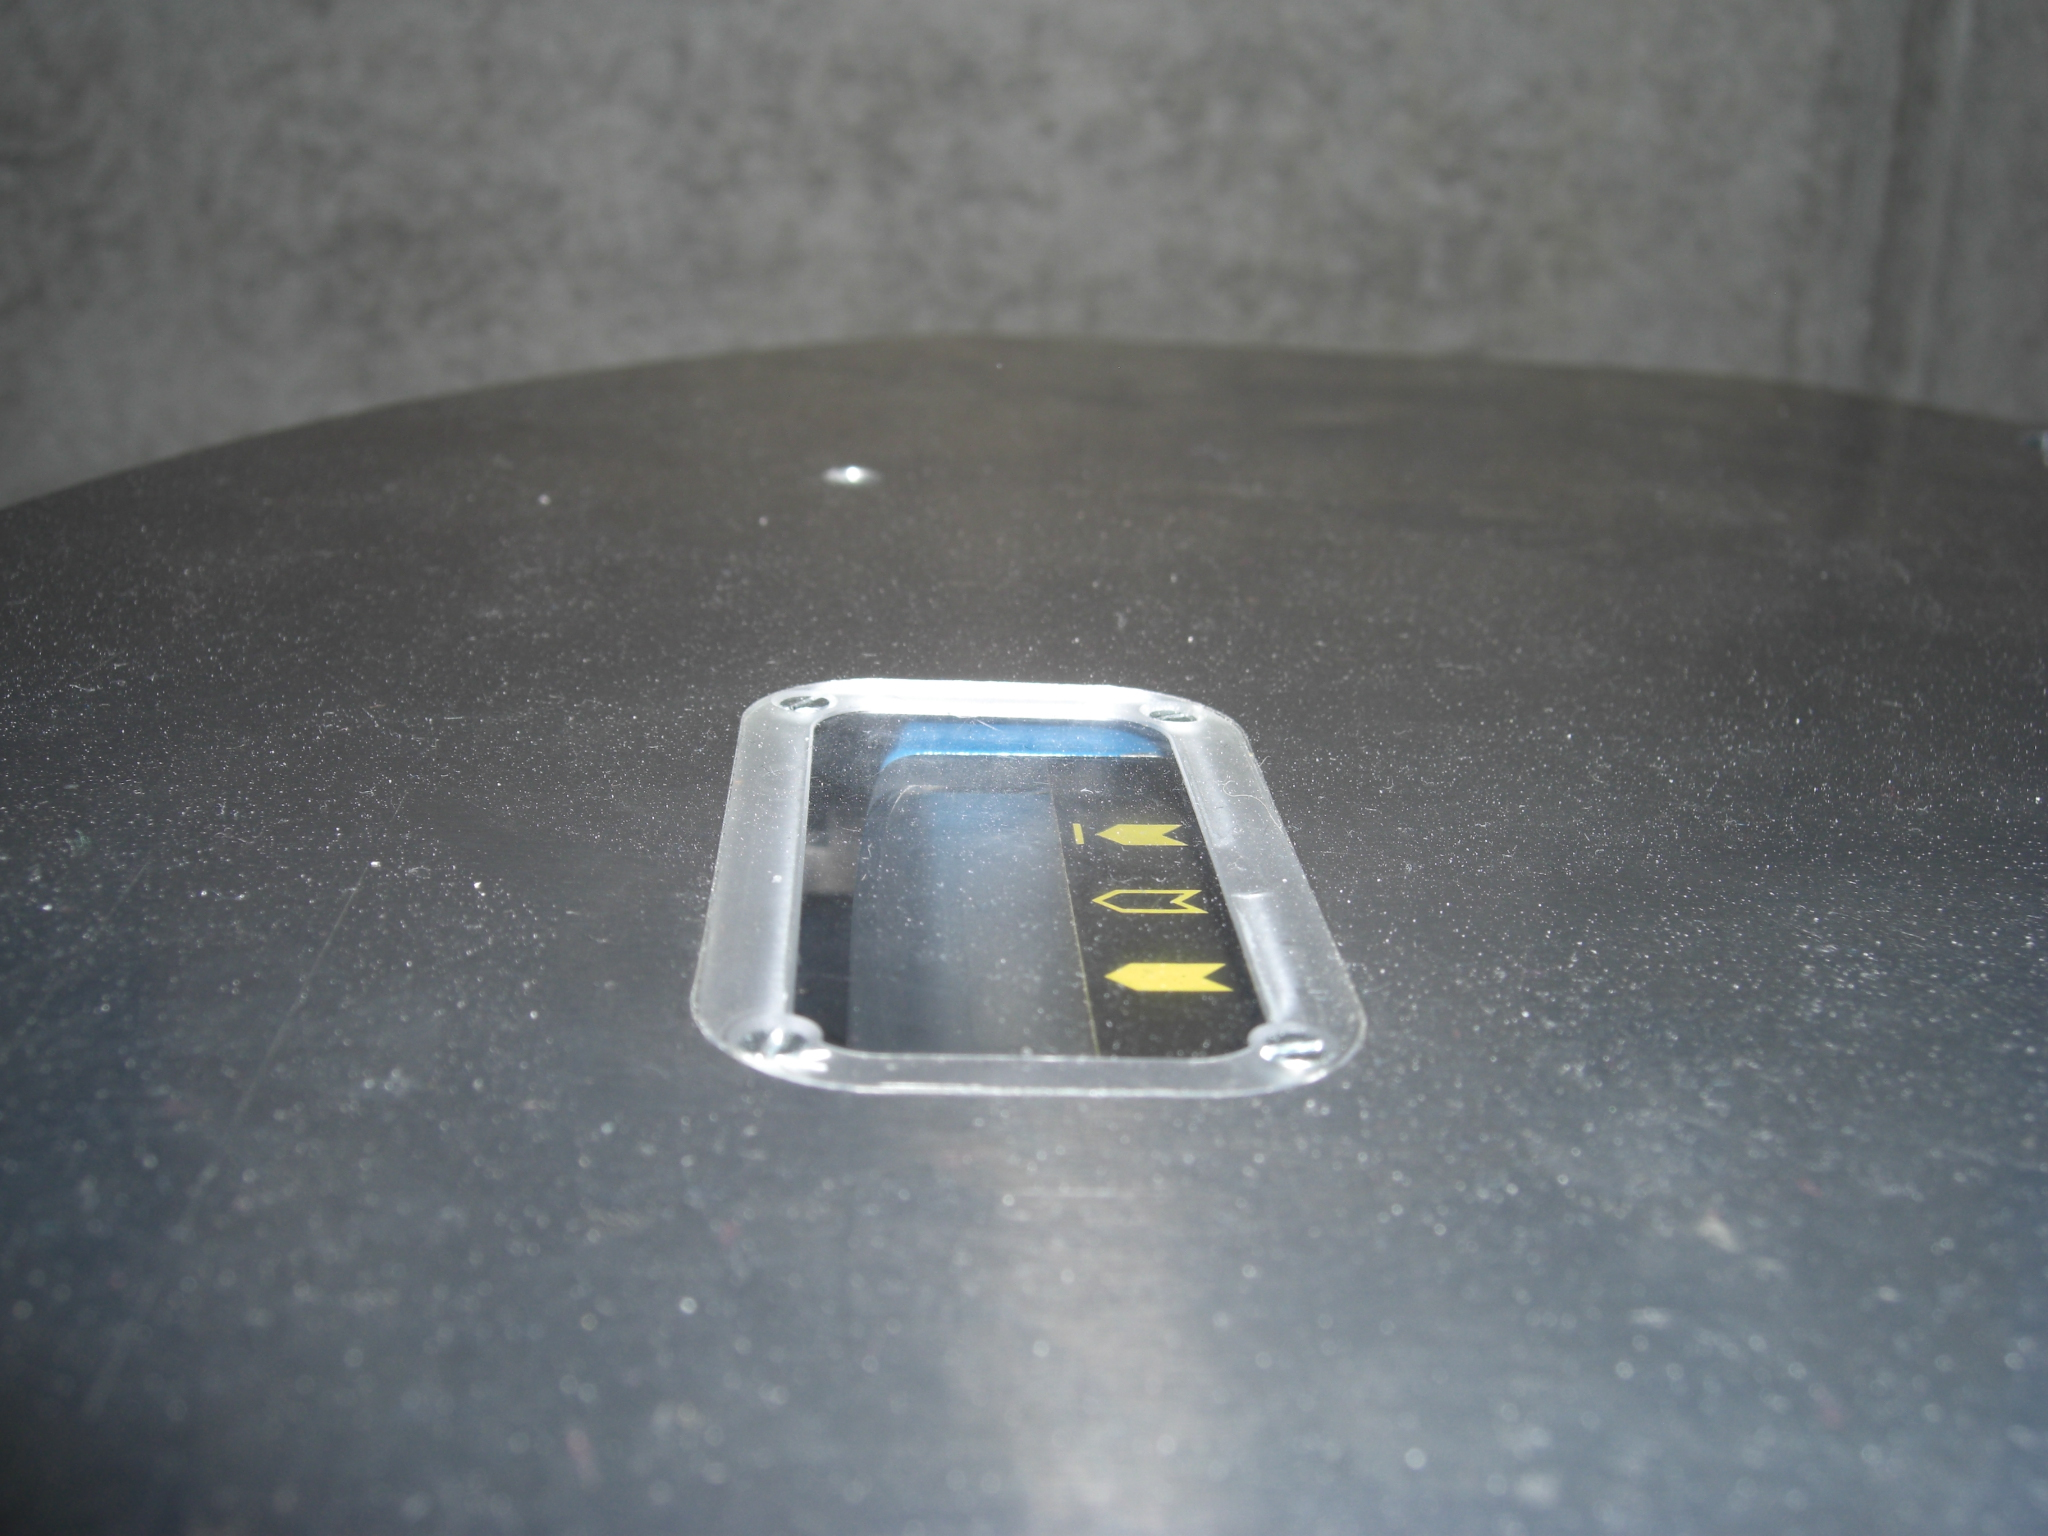
\includegraphics[width=\textwidth/2]{viewing_window.jpg}
  \caption{Viewing Window}
  \label{figure:viewingwindow}
\end{center}
\end{figure}
\begin{figure}[htp]
\begin{center}
  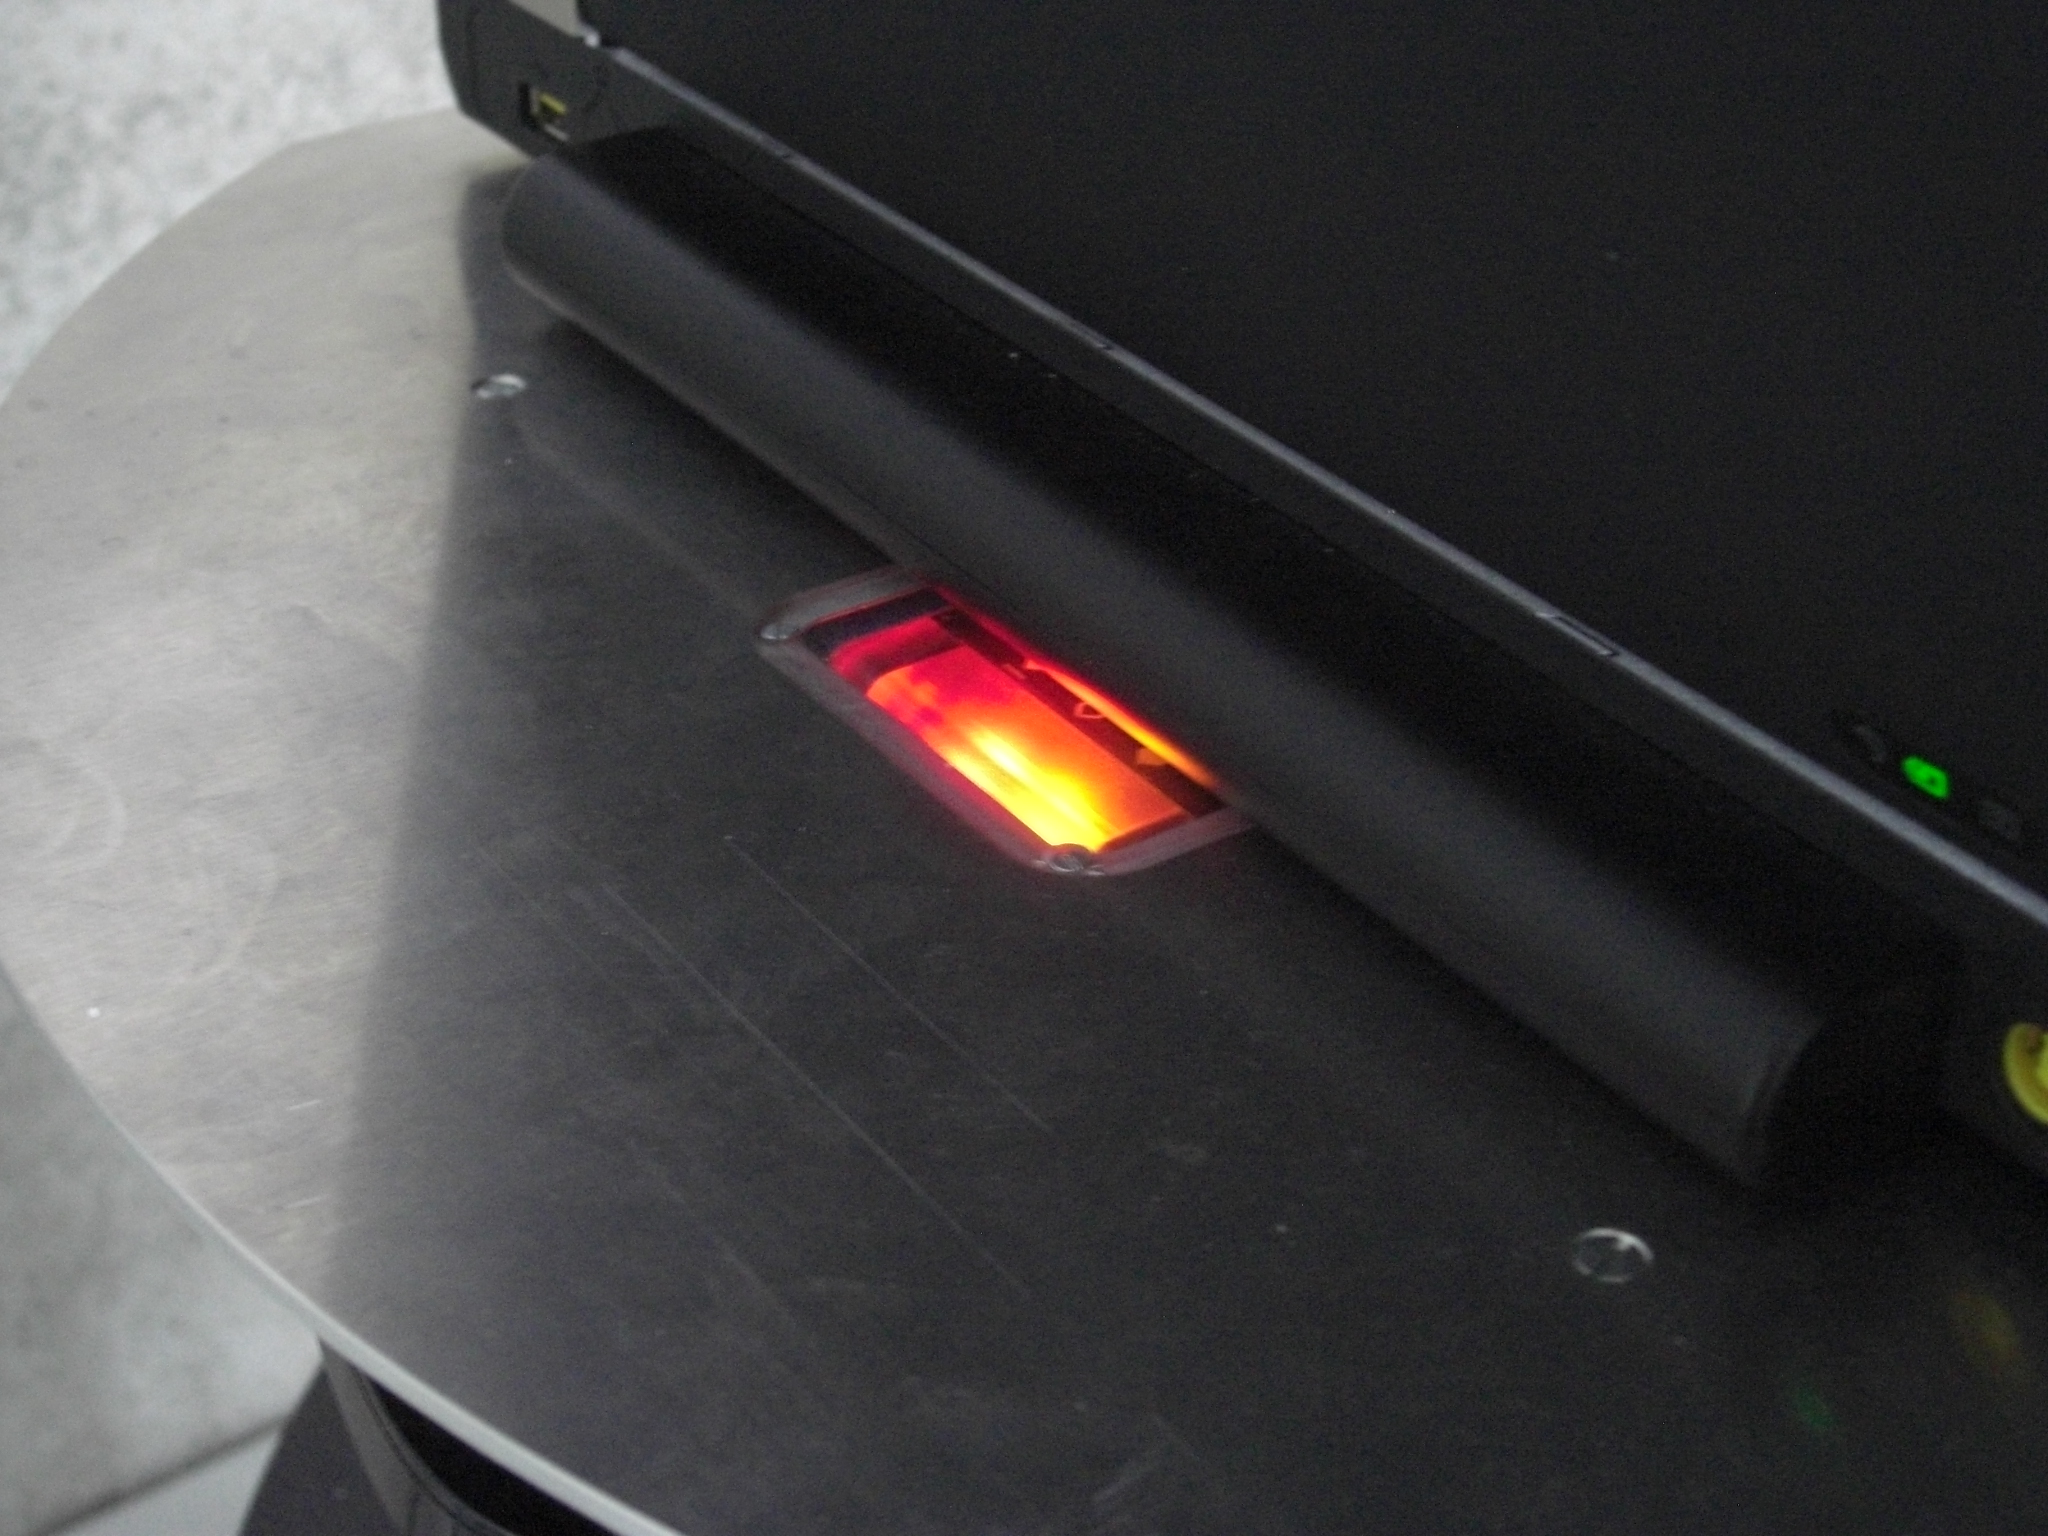
\includegraphics[width=\textwidth/2]{viewing_window_lt.jpg}
  \caption{Viewing Window (with Laptop)}
  \label{figure:viewingwindowlaptop}
\end{center}
\end{figure}
 
\chapter{Kinect Analysis}
\graphicspath{{./KinectData/img/}}

As mentioned in the introduction, a closer look to the Kinects data characteristics is taken
within this document to be able to implement a sign detection method. 
For this work the Kinect RAW fromat was used, each value has 16 bit and shows the
depth for the pixel in millimeters. A depth of zero means that no valid data is available for
this pixel.

\section{Surface Problems}

There are a few cases when the Kinect is not able to deliver any depth data from a surface.

First of all it does not work with translucent materials like glass. The projected
points are just fractured away, when they hit in a small angle (see figure \vref{figure:glas}). 
It's be possible to look through a translucent surface, but only if it's clear and the angle from the 
camera to the surface is not to big.
\begin{figure}[htp]
\begin{center}
  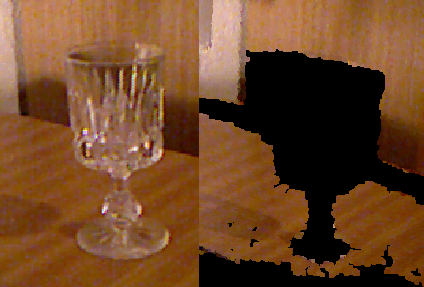
\includegraphics[height=\textheight/3]{glas.png} 
  \caption{Glass (Webcam/Pointcloud)}
  \label{figure:glas}
\end{center}
\end{figure}
 
Another problem are mirrors. Mirrors will also fracture the ir spots away, 
so it's not possible to get any depth data from their surfaces (see figure \vref{figure:mirror}).
\begin{figure}[htp]
\begin{center}
  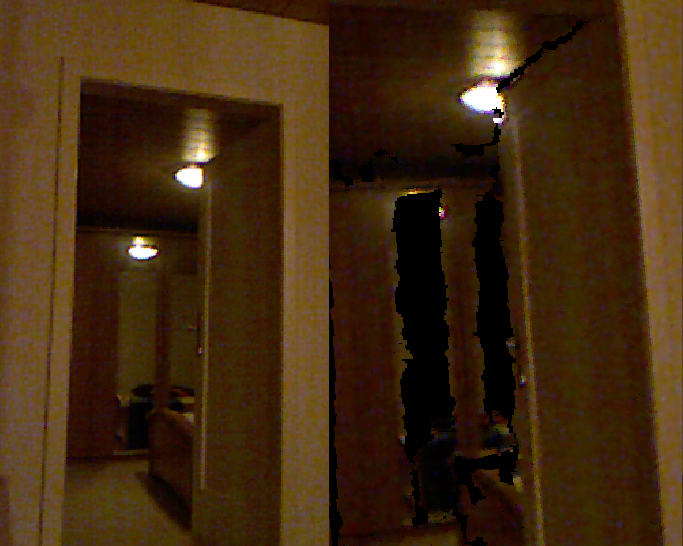
\includegraphics[height=\textheight/3]{Mirror.png}
  \caption{Mirror (Webcam/Pointcloud)}
  \label{figure:mirror}
\end{center}
\end{figure}

If the sun lights up a surface directly, it will outshine the ir-spots so this will blank out the surface
in the resulting depth image too (see figure \vref{figure:sun}).
\begin{figure}[htp]
\begin{center}
  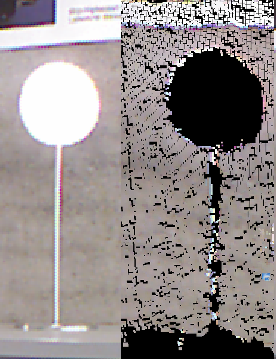
\includegraphics[scale=1.2]{Sun.png}
  \caption{Sunlight on a surface (Pointcloud/Webcam)}
  \label{figure:sun}
\end{center}
\end{figure}

On surfaces which are to close to the camera, the IR spots will melt together preventing the camera from
identifying their location (see figure \vref{figure:close}), what leads to the same result as in the previous cases.
\begin{figure}[htp]
\begin{center}
  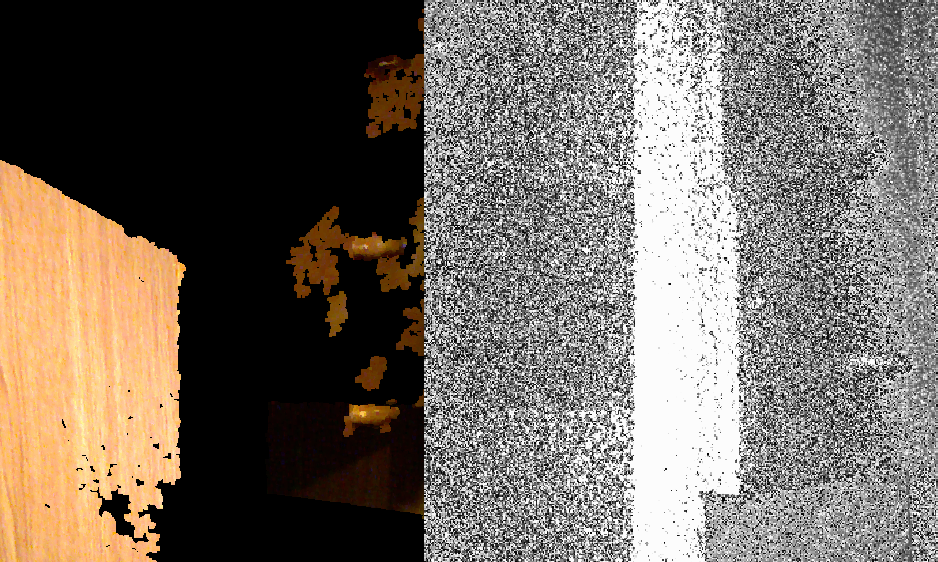
\includegraphics[scale=0.7]{ToClose.png} 
  \caption{Kinect to Close to a Surface (IR sensor/Pointcloud)}
  \label{figure:close}
\end{center}
\end{figure}
\clearpage

\section{Data Characteristics} 
 
\subsection{Analyzing Tools}

While this work multiple analyzing tools have been created. Those were created as
nodes to easily connect with the OpenNi driver package in the ROS system.

\subsubsection{DepthImageAnalyzer}
In the beginning a Qt-GUI node was created to get in touch with the depth images and 
their values and how they look like. It is able to show a depth image in the double
format and if the user clicks into the picture it will show the corresponding 
value of the pixel. It also allowed to set a depth range to highlight. 
Figure \vref{figure:DIA} shows the GUI of this node with a highlighted depth range.

\begin{figure}[h!tp]
\begin{center}
  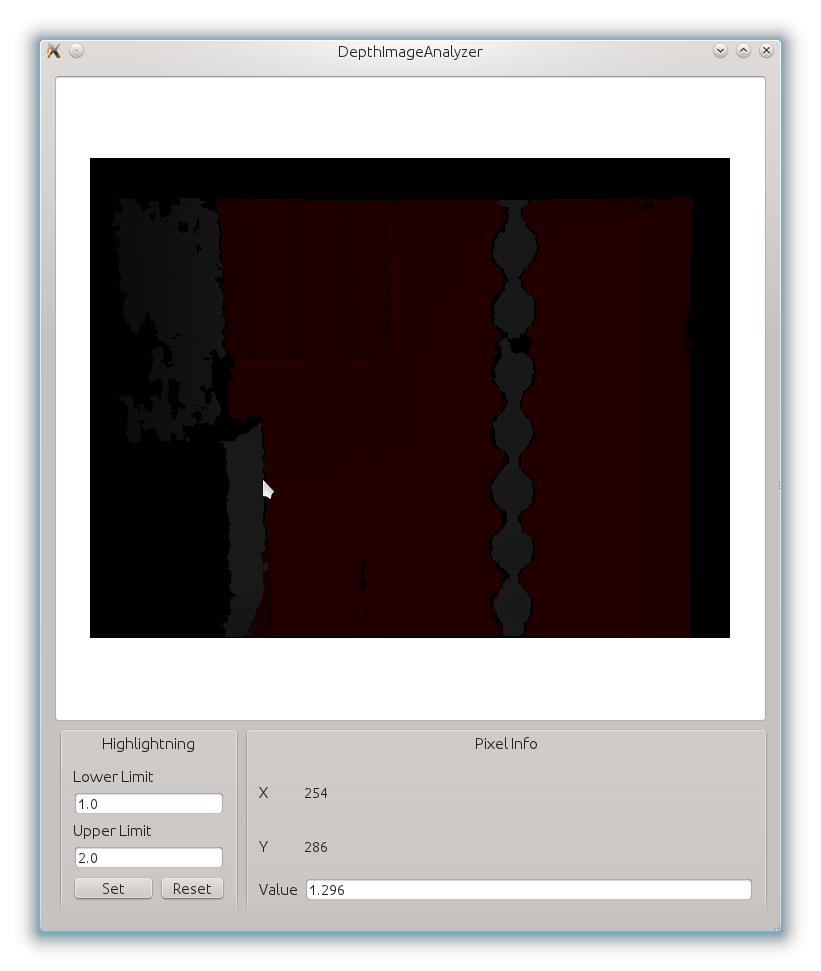
\includegraphics[width=\textwidth]{DepthImageAnalyzer.jpg}
  \caption{DepthImageAnalyzer GUI}
  \label{figure:DIA}
\end{center}
\end{figure}
\clearpage 


In the later process of this work it was not needed anymore, because showing the point cloud
in rViz showed to be more effective in analyzing data and debugging applications.

\subsection{PointCloud creation with selected topics}
Point clouds are very useful for debuging and filtering techniques. They can be displayed in
3D and directly show what happens to the data when a special filter is applied.
To create point cloud messages for other topics than those from the Kinect node it is necessary to
create specific launch files. Launch files are xml-files which are used to start multiple nodes in one
go. 


\begin{lstlisting}[caption={Standalone Point Cloud}\label{lst:stal_pcl},language=xml]
<!-- Nodelet for creating a pointcloud out of the detector image (for debuging filters) -->
<node pkg="nodelet" type="nodelet" name="PointCloudAdvisor" args="manager" output="screen"/>

<node pkg="nodelet" type="nodelet" name="points_xyzrgb_Advisor" 
	args="load depth_image_proc/point_cloud_xyzrgb PointCloudAdvisor --no-bond">
    <remap from="rgb/image_rect_color"        to="/signDetection/out_rgb" />
    <remap from="rgb/camera_info"             to="/signDetection/camera_info" />
    <remap from="depth_registered/image_rect" to="/signDetection/out_depth" />
    <remap from="depth_registered/points"     to="debug_cloud" />
</node>
\end{lstlisting}



As seen in the listing for creating a point cloud from different topics a nodelet manager and a 
depth\_image\_proc/point\_cloud\_xyzrgb nodlet is needed. Inside the node tag of the nodelet
there are the remapping tags, to connect the nodelet with the custom topics.

\subsection{Tool for various data fetching and filter testing}
The tool was named disturbance\_filter\_calculator, the name is still reminding what it was intended to do. It should
filter out the noise by creating a picture of it on a flat surface. This didn't work because of the special autoranging
feature of the Kinect which will be discussed later. Currently the Tool can be used to fetch data points or to
draw a pattern of lines in the RGB image which is mapped over the point cloud. It also can tell the users which data points
are in a given distance and which not by painting the pixels of the RGB image green for being in the specified distance
and red if not. This feature helped to realize about the missing values which are also discussed later. It also includes
some of the first tries to filter and blur the depth image, but as the project advanced it was decided to move the 
filter code to a new clean node in a new package to save compiling time, leaving the disturbance\_filter\_calculator 
node as it was.

%TODO pictures filter_calculator

\section{Disturbances}
While pointing the Kinect to a flat surface the noise fractals (see in figure \vref{figure:noise}) 
seem to reappear at the same position. So it was decided to try to remove them with capturing a image from a flat surface.
and subtract the number of data steps the noise produces. Therefore the kinect is arranged very close to a flat surface 
so that it only will see this surface. Then a picture is created which stores the difference of the data to the 
distance of the surface to be substracted from the following frames.
This was a nice idea but it didn't work as expected. There some special vertical fractals (see in figure \vref{figure:verticals}) 
inside the data which seem to be the result from an autoranging feature of the camera, 
always creating one data step in the picture. The biggest problem is that the scale of the noise fractals changes 
with their appearance and their number. The number of those vertical lines ranges from 0 to a spotted maximum of 9. 
They do always appear on a special range, seem to be symetrical or 
nearly symetrical to the center and their number is never even but are not fixed to a special column of pixels. 
\begin{figure}[htp]
\begin{center}
  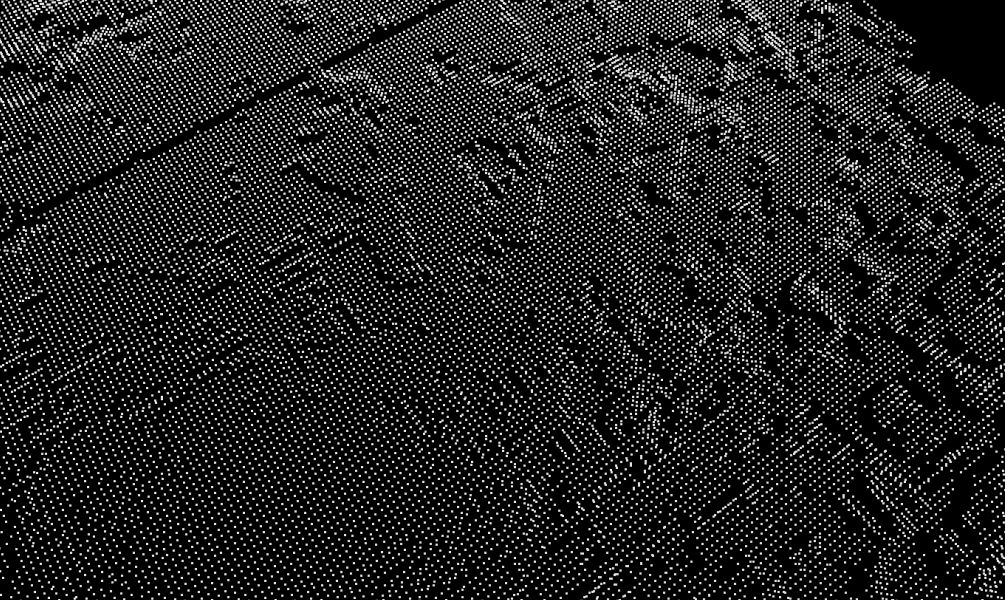
\includegraphics[width=\textwidth]{noise.png}
  \caption{Noise (Pointcloud)}
  \label{figure:noise}
\end{center}
\end{figure}

\begin{figure}[htp]
\begin{center}
  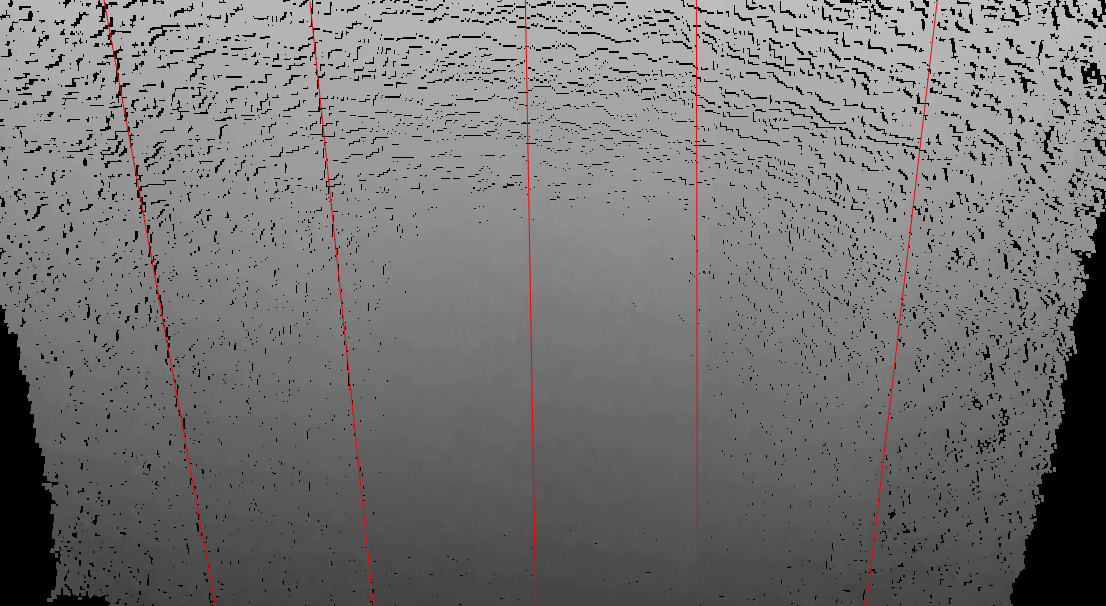
\includegraphics[width=\textwidth]{verticalFractals.png}
  \caption{Vertical Fractals (Pointcloud)}
  \label{figure:verticals}
\end{center}
\end{figure}

\section{Resolution Depending the Depth} \label{resdepDepth}
When creating the diagram (in figure \vref{figure:LaserKinect}) which shows the occuring values from the camera 
at a specific distance from a plane and parallel surface and the distance measured with a laser distance measurement 
device(see in figure \vref{figure:hilti}),it was realized that many values just do not exist. The camera does never output 
these values. After realizing this fact it was decided to look for the available values, their number and the values which 
never occur.The figures \vref{figure:depths1} and \vref{figure:depths2} show the distance on the left, 
the available values (black) and not availabe values (white) in the middle and the number of the missing values between them 
on the right. Figure \vref{figure:DepthValueDiff} shows the number of missing values in relation to the depth.

\begin{figure}[htp]
\begin{center}
  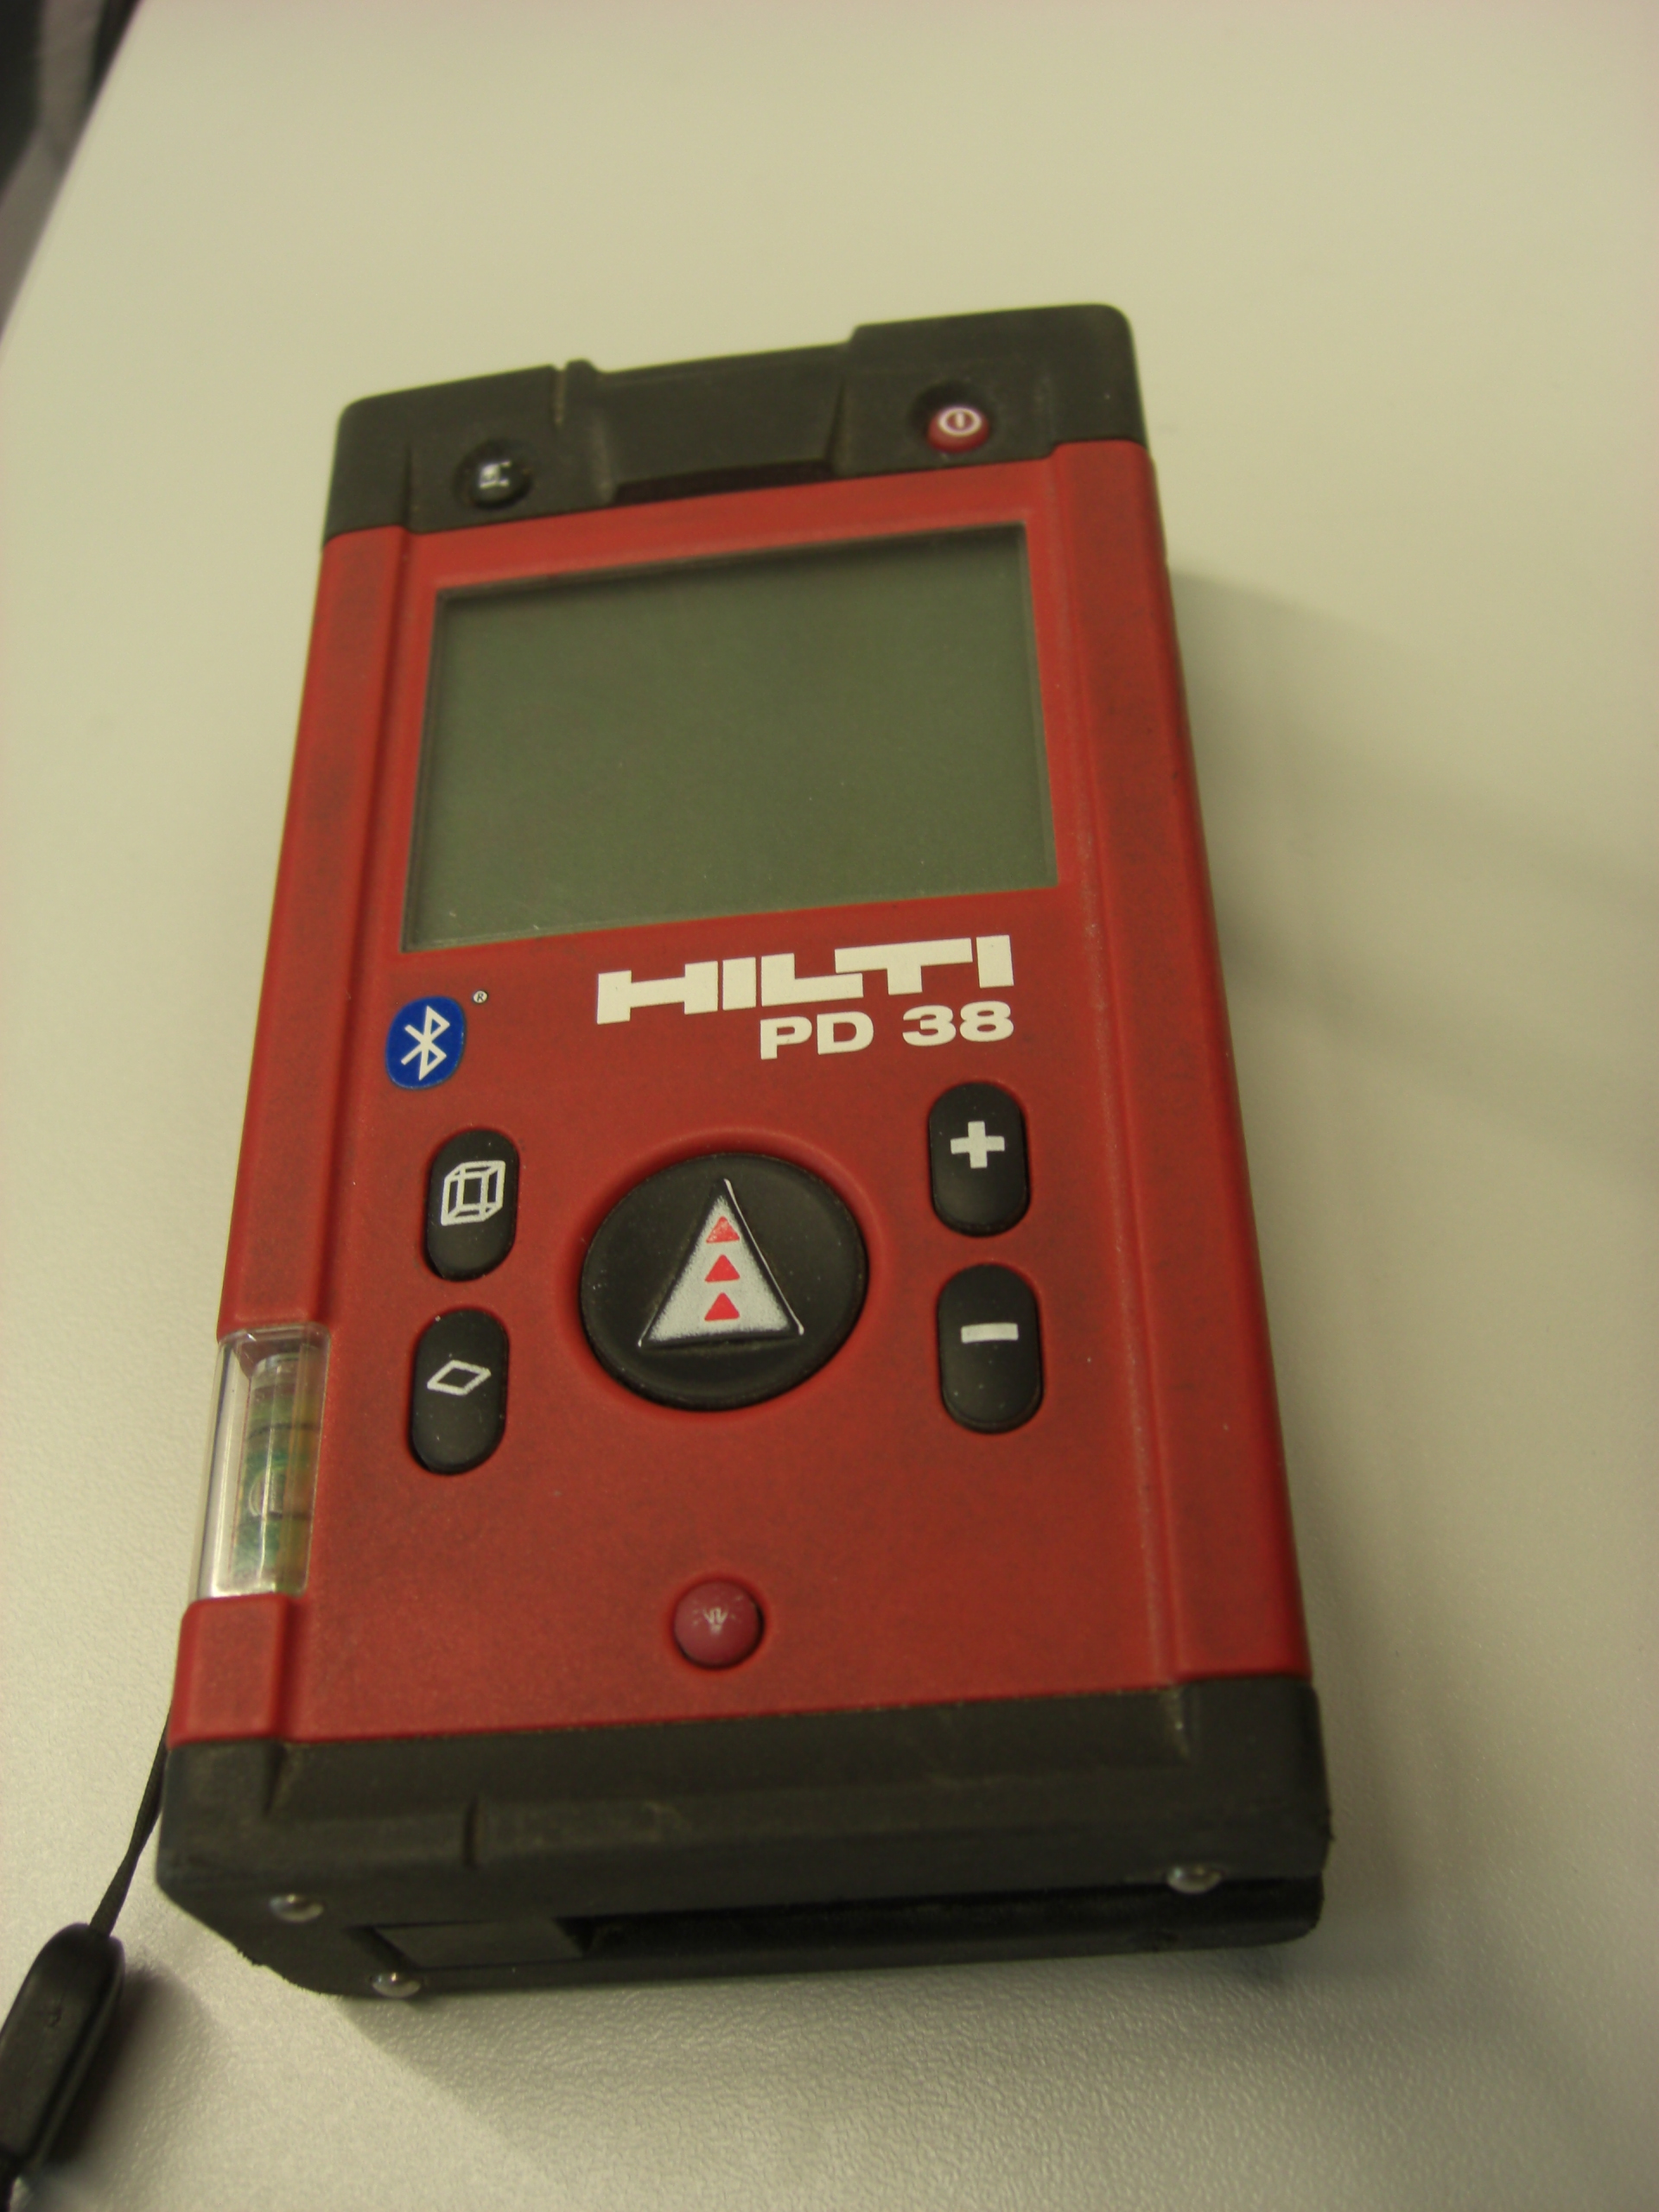
\includegraphics[width=\textwidth/4]{hiltipd38.jpg}
  \caption{Hilti PD38 Laser Distance Measurement Device}
  \label{figure:hilti}
\end{center}
\end{figure}
\begin{figure}[htp]

\begin{center}
  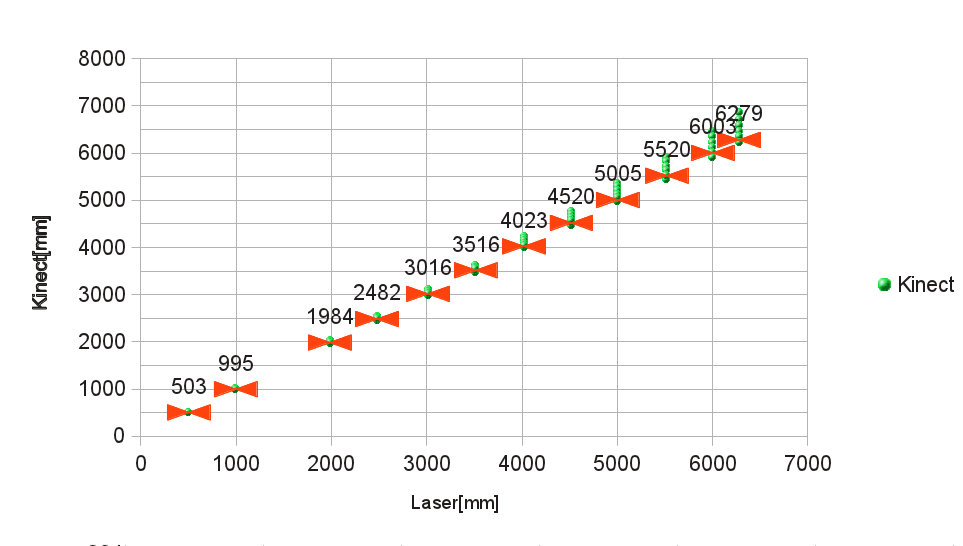
\includegraphics[scale=0.8]{LaserDistanceKinectDistance.png}
  \caption{Distance measured by Laser and by Kinect}
  \label{figure:LaserKinect}
\end{center}
\end{figure}

\begin{figure}[htp]
\begin{center}
  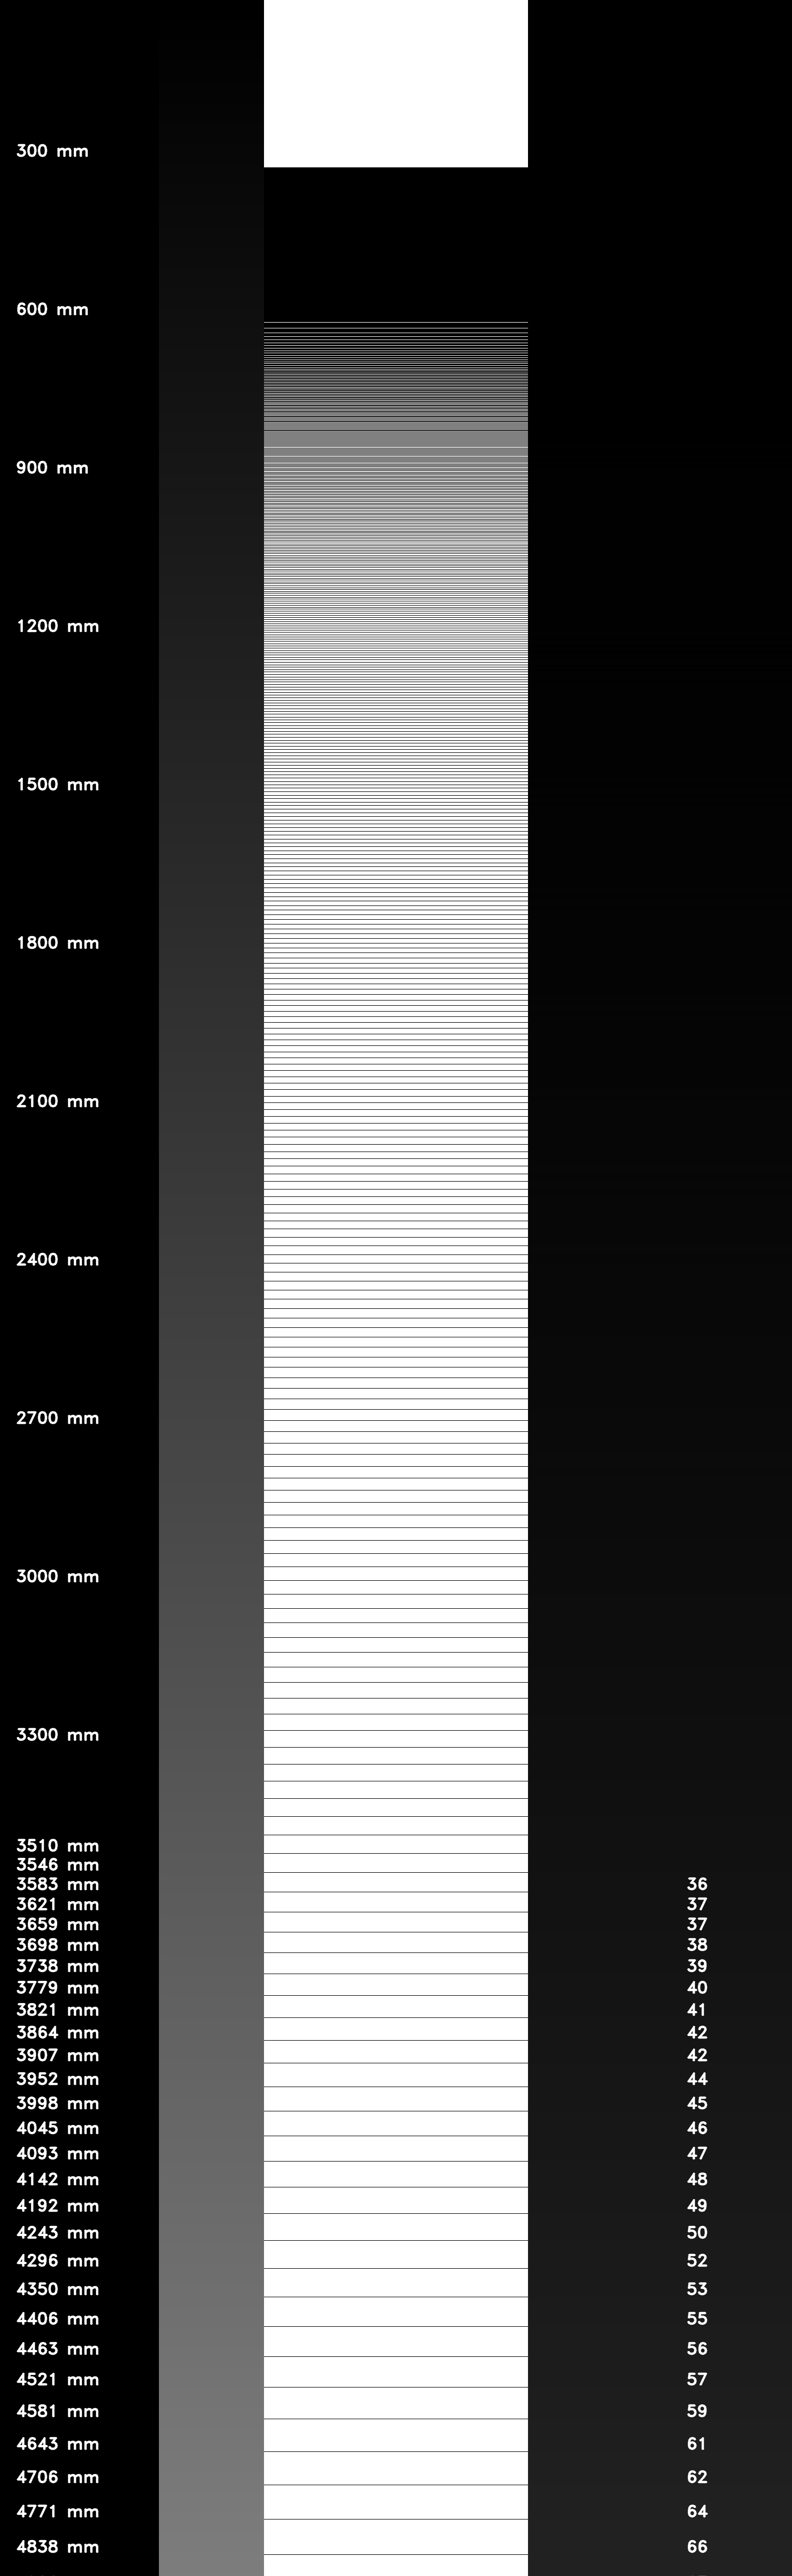
\includegraphics[scale=0.1]{availdepths0.png}
  \caption{Available Depth Values from 0 to 4,8 m}
  \label{figure:depths1}
\end{center}
\end{figure}

\begin{figure}[htp]
\begin{center}
  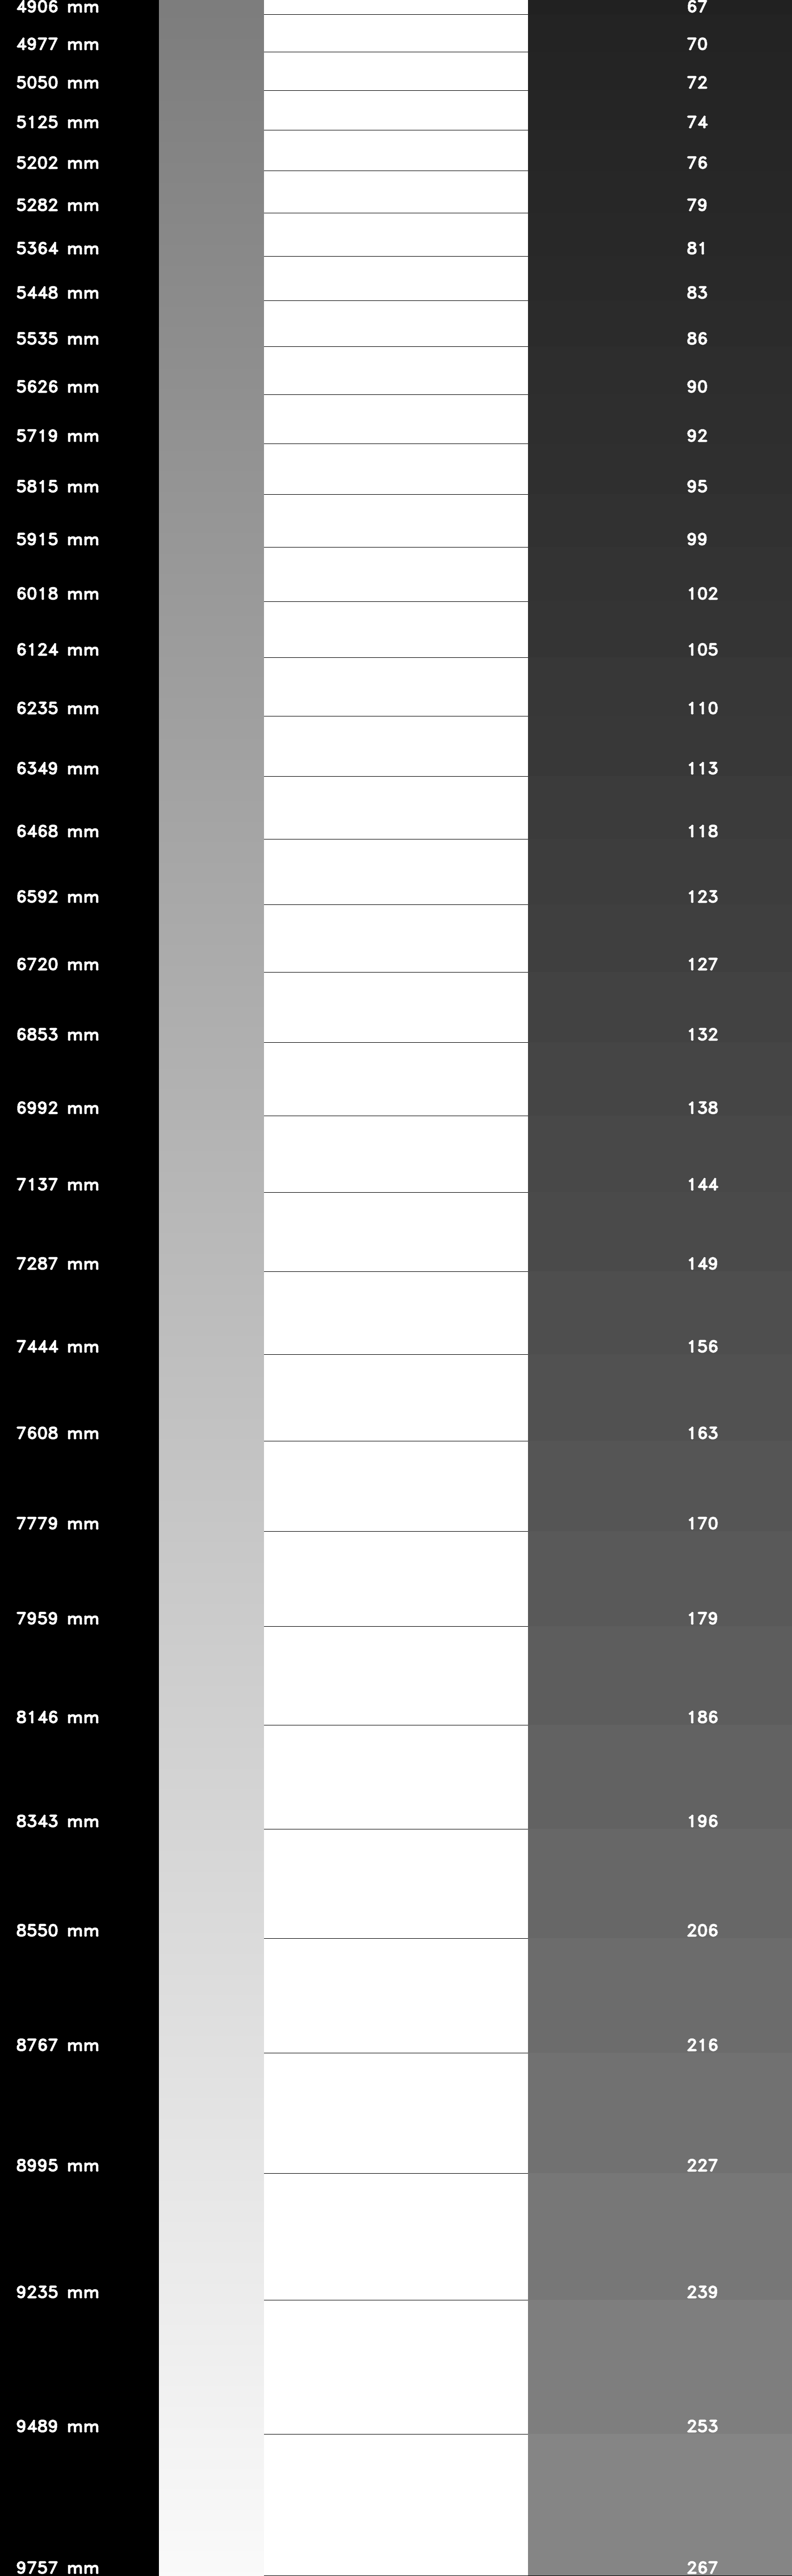
\includegraphics[scale=0.1]{availdepths1.png}
  \caption{Available Depth Values from 4,8 m to 9,8m}
  \label{figure:depths2}
\end{center}
\end{figure}

\begin{figure}[htp]
\begin{center}
  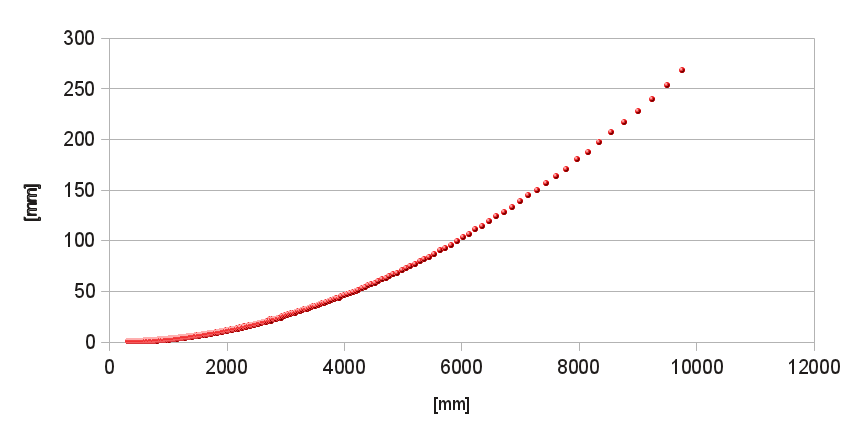
\includegraphics[width=\textwidth]{DifferenceForegoing.png}
  \caption{Missing values in relation to the depth}
  \label{figure:DepthValueDiff}
\end{center}
\end{figure}

\graphicspath{{./Software/img/}}
\chapter{Sign Recognition}\label{chapter:SignRecognition}
 
 Before being able to do filtering, detect signs etc, it is necessary to get the data from the OpenNi nodletmanager,
 the node which supplies the depth and RGB data. Therefore the code for synchronizing RGB, 
 depth and camera info messages was copied from the nodelet being responsible 
 for point cloud creation. 
 
To connect the node with the necessary topics of the OpenNi node, the launchfile in listing \vref{lst:launch}
was used. It also creates a point cloud for debugging output of the processed data.

\begin{lstlisting}[caption={Project Launch File}\label{lst:launch},language=xml]
<launch>

	<param name="/camera/driver/depth_registration" value="true" />	

	<!-- Launch a reconfigure GUI -->
	<node pkg="dynamic_reconfigure" type="reconfigure_gui" 
	name="reconfigure_gui" output="screen" respawn="true"  />
	
	
	<!-- Start the camera-->
	<include file="$(find openni_launch)/launch/openni.launch" />
	<node pkg="rviz" type="rviz" name="rviz_signDetect" output="screen" 
	respawn="true"  />

	<!-- SignDetector -->
	<node pkg="aa_signs" type="signDetection" name="signDetection" 
	 output="screen" respawn="true" > 
 		<remap from="/signDetection/depth_registered/image_rect" 	
 		to="/camera/depth_registered/image_rect_raw" />
 		<remap from="/signDetection/rgb/image_rect_color" 			
 		to="/camera/rgb/image_rect_color" />
 		<remap from="/signDetection/rgb/camera_info" 				
 		to="/camera/rgb/camera_info" />
 		<param name="settingsfile" value="(find aa_signs)/settings/signs.xml" />
	</node>

  	<!-- Nodelet for creating a pointcloud out of the detector image-->
	<node pkg="nodelet" type="nodelet" name="PointCloudAdvisor" 
	args="manager" output="screen"/>

		<node pkg="nodelet" type="nodelet" name="points_xyzrgb_Advisor" 
		args="load depth_image_proc/point_cloud_xyzrgb PointCloudAdvisor --no-bond">
	    <!-- Explicit topic remappings, shouldn't need all of these -->
	    <remap from="rgb/image_rect_color"        to="/signDetection/out_rgb" />
	    <remap from="rgb/camera_info"             to="/signDetection/camera_info" />
	    <remap from="depth_registered/image_rect" to="/signDetection/out_depth" />
	    <remap from="depth_registered/points"     to="debug_cloud" />
  	</node>
  	
  	
</launch>
\end{lstlisting}

\section{Depth Image Processing}
Before trying to do template matching in the camera image, it's necessary to limit the regions in which we are
searching for known templates. Therefore it is necessary to find surfaces which are upright to the camera view.
In beginning the focus in almost any image processing project lies on improving image quality by removing the 
noise and this is also the case for this project.

\subsection{First Blur Filter}
Bluring the depth image to remove the noise sounds like an easy task, but if a boxed filter is used 
all edges are smoothed with surfaces they do not belong to (see first picture in figure \vref{figure:blur}).
At first it was tried to do all the filtering and reset all blured pixels $P_b$ which are to far away from their 
original depth value $P$ by equation \ref{eq:resetPix}.
 
\begin{equation}
   \left(\left|{P_b(x,y)-P(x,y)}\right|>{\frac{P(x,y)^2}{480000}}\right)\implies P_b(x,y)=P(x,y)
   \label{eq:resetPix}
\end{equation}

Listing \vref{lst:fstBlur} shows the code of this first filter, which used a box-filter
(kernel shown in equation \vref{eq:boxedKernel} as said in manual \cite{willowgarage:opencv:boxed})

\begin{equation}
	K=\frac{1}{7*3}
	\begin{bmatrix} 1 & 1 & 1 & 1 & 1 & 1 & 1\\ 
					1 & 1 & 1 & 1 & 1 & 1 & 1\\ 
					1 & 1 & 1 & 1 & 1 & 1 & 1 
	\end{bmatrix}
	\label{eq:boxedKernel}
\end{equation}

and a median-blur filter with an $3 \times 3$ aperture. In the next step equation \ref{eq:resetPix} is used 
to revert pixels. Then another blur filter, with the same aperture size as before, 
is applied to remove possible noise resulting from reseting the pixels (see figure \vref{figure:blur} for results).

\begin{lstlisting}[caption={Code of the first Bluring Function}\label{lst:fstBlur},language=c++]
void myFilter1(const cv::Mat &src, cv::Mat &dst)
{
	cv::Mat filter_in = src.clone();
	cv::Mat filter=filter_in.clone();
	cv::boxFilter(filter, filter, 3, cv::Size(7, 3), cv::Point(-1, -1), 1, 0);
	cv::medianBlur(filter, filter, 3);
	
	//Update non zero pixels
	for (int y = 0; y < src.rows; y++)
	{
		for (int x = 0; x < src.cols; x++)
		{
			short realValue = filter_in.at<Vec1shrt>(y, x)[0];
			short filteredValue = filter.at<Vec1shrt>(y, x)[0];
			short maxDifference = pow((float)realValue, 2) / (480000);
			if (realValue>0)
			{
				if(abs(realValue - filteredValue) > maxDifference)
				{
					dst.at<Vec1shrt>(y, x)[0] = realValue;
				}
				else
				{
					dst.at<Vec1shrt>(y, x)[0] = filteredValue;
				}
			}
		}
	}
	cv::medianBlur(dst, dst, 3);
}
\end{lstlisting}

\begin{figure}[H]
\begin{center}
  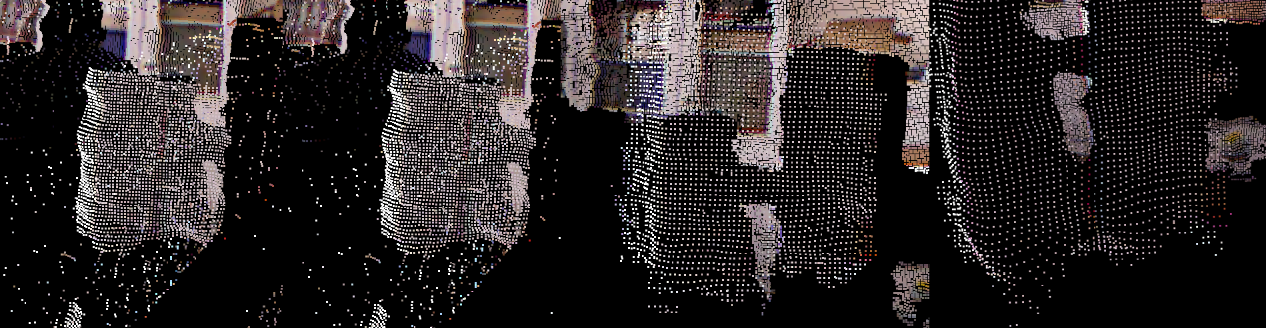
\includegraphics[width=\textwidth]{myFilter1.png}
  \caption[Blur Filter Steps]{Blur Filter Steps(1.Boxed/2.Median/3.Reseting Borders/4.Median)}
  \label{figure:blur}
\end{center}
\end{figure}

\subsection{Neighborhood Map and New Blur Filter} \label{sect:blurFilter} 
After realizing that there are only 824 depth values available, it was decided to transform the depth picture
to the available depth steps. The resulting step map contains the number of each available depth. 
The converting function uses an array. This array contains the number of the
step when obtaining the cell number of its value. Each cell of a non-existing value contains -1, so it is
possible to check if something is wrong with the value and if it is not an Kinect RAW picture.
In table \vref{table:Kinect2Step} an abridgement from the look-up table is shown in table \vref{table:Kinect2Step}
(without the missing fields mentioned before) and listing \vref{lst:stpmap} contains the code of the converting function.


\begin{table}[H]
\centering
\tiny
\begin{tabular}{lccccccccccccccc}
Kinect Depth& 0 & 317 & 318 & 319 & 320 & 321 & ... & 8146 & 8343 & 8550 & 8767 & 8995 & 9235 & 9489 & 9757\\
Step Number & 0 &   1 &   2 &   3 &   4 &   5 & ... &   817 & 818 &  819 &  820 &  821 &  822 & 823  & 824\\
\end{tabular}
\caption{Abridgement from Kinect Depth to Step Number Look-Up Table }
\label{table:Kinect2Step}
\end{table}


\textbf{Example:}

Assuming table \vref{table:ConvExampleKinect} is an image from a Kinect camera, 
table \vref{table:ConvExampleStep} would show the corresponding step map when using the look-up table \vref{table:Kinect2Step}.

\begin{table}[H]
\centering
\huge
\begin{tabular}{ccc}
0 & 320 & 321\\
8146 & 8550 & 9489\\
\end{tabular}
\caption{Example: Kinect to Step Map: Kinect Image}
\label{table:ConvExampleKinect}
\end{table}

\begin{table}[H]
\centering
\huge
\begin{tabular}{ccc}
0 & 4 & 5\\
817 & 819 & 823\\
\end{tabular}
\caption[Example: Corresponding Step Map]{Example: Corresponding Step Map (from table \vref{table:ConvExampleKinect})}
\label{table:ConvExampleStep}
\end{table}

\begin{lstlisting}[caption={covertKinectRawToSteps - Function}\label{lst:stpmap}, language=c++]
void convertKinectRawToSteps(const cv::Mat &src, cv::Mat &dst)
{
	if(src.type() == CV_16UC1)
	{
		dst=src.clone();

		int size_x=src.cols, size_y=src.rows;

		for (int i = 0; i < (size_x*size_y); i++)
		{
			//Forward direction x -
			int y_xfw=i/size_x, x_xfw=i-y_xfw*size_x;
			short current=src.at<Vec1shrt>(y_xfw,x_xfw)[0];
			if(current>=0 && current < kinect_depths_count)
			{
				if(kinect_depth_to_step_LUT[current]>=0)
				{
					dst.at<Vec1shrt>(y_xfw,x_xfw)[0]=kinect_depth_to_step_LUT[current];
				}
				else
				{
					std::cerr<<"convertKinectRawToSteps: Unregistered Depth Value found!" 
					           " You must use unedited KINECT RAW data for this! "
							 <<"Value is: "<<current<<std::endl;
				}
			}
			else
			{
				std::cerr<<"convertKinectRawToSteps: Unregistered Depth Value found " 
				           "(too big)! You must use unedited KINECT RAW data for this! "
						 <<"Value is: "<<current<<std::endl;
			}
		}
	}
	else
	{
		std::cerr<<"convertKinectRawToSteps: Wrong matrix type! "
		"You must use unedited KINECT RAW (CV_16UC1) data for this! "<<std::endl;
	}
}
\end{lstlisting}


\newpage
With that new image it's now possible to determine if a pixel is a direct neighbor to another one. This is mostly the case,
when the value from the difference of the steps is smaller than or equal to one. A threshold of four is adequate to be sure 
to eliminate the noise created by the fractals (shown in figure \vref{figure:noise}) 
which can create a step difference of up to 3 inside a surface. So the value of a pixel $P_n$ in the neighborhood map
can be determined as seen in equations \vref{eq:neighbors_xi} to \vref{eq:neighbors}, where $b_i$ is a bit of this value, 
$S$ the value of a pixel in the step map, while $u$ and $v$ represent the width and height of the image. With this procedure 
a neighborhood map is created which contains a 8-bit value for each pixel, where each bit shows the neighborhood 
condition to one of the eight pixels $(x_i,y_i)$ around the current one(x,y). An example and the numbering of the pixels $i$ 
can be seen in figure \vref{figure:neighborhoodmap}.

\begin{equation}
 x_i = \left\{ 
	 \begin{array}{ll}
	         x   & i \in \{1,5\} \\
	         x+1 & i \in \{2,3,4\} \\
	         x-1 & i \in \{0,6,7\} 
	 \end{array} 
\right.        
\label{eq:neighbors_xi} 
\end{equation}


\begin{equation}
 y_i = \left\{ 
	 \begin{array}{ll}
	         y   & i \in \{3,7\} \\
	         y+1 & i \in \{4,5,6\} \\
	         y-1 & i \in \{0,1,2\} 
	 \end{array} 
\right.        
\label{eq:neighbors_yi} 
\end{equation}



\begin{equation}
 b_i = \left\{ 
	 \begin{array}{ll}
	         1 & \left|S(x_i,y_i)-S(x,y)\right|<4  \wedge   S(x_i,y_i) \neq 0 \wedge 0<=x_i<u  \wedge 0<=y_i<v\\
	         0 & \mbox{otherwise} 
	 \end{array}
\right.        
\label{eq:neighbors_bit} 
\end{equation}

\begin{equation}
	P_n(x,y)=\sum_{i=0}^7 2^i \cdot b_i \mbox{\hspace{1cm}(True for $0<=x<u$ and $0<=y<v$)}
\label{eq:neighbors} 
\end{equation}

\begin{equation}
	P_n(x,y)=\sum_{i=0}^7 (b_i)\mbox{LEFT-SHIFT-BY-$i$ \hspace{0.5cm} (used in code, same result as equation \ref{eq:neighbors})}
\label{eq:neighbors_cpp} 
\end{equation}
 
 

\begin{figure}[H]
\begin{center}
  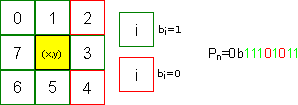
\includegraphics[width=\textwidth]{neighborhoodmap.pdf}
  \caption{Neighborhood-Map Example for One Pixel}
  \label{figure:neighborhoodmap}
\end{center}
\end{figure}

This information helps to write a more performance saving, effective and edge saving bluring method which 
was named crossBlur, because it blures each pixel with a specified number of it's neighbors on top, left, right and bottom.
The neighborhood condition is needed, because it will stop adding pixels on each side if the next pixel in the direction 
is not a close neighbor to the current, to preserve the edges. (see in figure \vref{figure:crossblur}).

\begin{figure}[H]
\begin{center}
  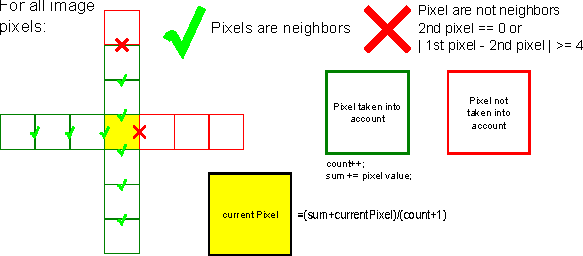
\includegraphics[width=\textwidth]{crossBlur.pdf}
  \caption{Cross Blur Working Principle}
  \label{figure:crossblur}
\end{center}
\end{figure} 



Algorithm \vref{alg:crossblur} represents the pseudo code, where $b_1$, $b_3$, $b_5$
and $b_7$ are the bits for the neighborhood condition to the top, left, bottom and right pixel
of the given coordinates (previously calculated with equation \vref{eq:neighbors_bit}). While
$d$ is the amount of pixels to be taken into account at a maximum on each side, $j$ refers to the control
variable.  $D_{in}$ and $D_{out}$ are pixels inside the input and the ouput depth image.

Listing \vref{lst:crossblur} is showing the cross bluring function in C++ and figure \vref{figure:crossblurResult} 
displays a result.


\begin{algorithm}[H]

	\begin{algorithmic}
\ForAll{x,y} 
	\State {$b_t \gets b_1(x,y) $}
	\State {$b_r \gets b_3(x,y) $}
	\State {$b_b \gets b_5(x,y) $}
	\State {$b_l \gets b_7(x,y) $}
	\State {$sum \gets D_{in}(x,y)$}
	\State {$cnt \gets 1$}
	
	\For{$j=0 \to d$} 
		\If {b$_t = true$} 
			\State {$b_t \gets b_1(x,y-j)$}
			\State {$sum \gets sum+D_{in}(x,y-j)$}
			\State {$cnt \gets cnt+1$}
		\EndIf
		\If {b$_r = true$} 
			\State {$b_r \gets b_3(x+j,y)$}
			\State {$sum \gets sum+D_{in}(x+j,y)$}
			\State {$cnt \gets cnt+1$}
		\EndIf
		\If {b$_b = true$} 
			\State {$b_b \gets b_5(x,y+j)$}
			\State {$sum \gets sum+D_{in}(x,y+j)$}
			\State {$cnt \gets cnt+1$}
		\EndIf
		\If {b$_l = true$} 
			\State {$b_l \gets b_7(x-j,y)$}
			\State {$sum \gets sum+D_{in}(x-j,y)$}
			\State {$cnt \gets cnt+1$}
		\EndIf 
		\State{$D_{out}(x,y) \gets \frac{sum}{cnt}$}
	\EndFor
\EndFor

	\end{algorithmic}
 \caption{Cross Blur}
 \label{alg:crossblur}
\end{algorithm}



\begin{lstlisting}[caption={crossDepthBlur - Function}\label{lst:crossblur}, language=c++]
void crossDepthBlur(const cv::Mat &depth, const cv::Mat &neighbors, 
                    cv::Mat &depth_out, int max_size)
{
	cv::Mat dst=cv::Mat::zeros(depth.rows,depth.cols,CV_16UC1);
	int size_x=depth.cols, size_y=depth.rows;
	int y,x;
	for (int i = 0; i < (size_x*size_y); i++)
	{
		y=i/size_x;
		x=i-y*size_x;

		//Sum all pixels
		int sum=depth.at<Vec1shrt>(y, x)[0];

		//If current pixel is 0 go to next
		if(sum == 0) continue;

		//Count all values
		int cnt=1;

		//Get the neighbors of the current pixel
		uchar cur_nb=neighbors.at<Vec3uchar>(y,x)[0];

		//Usable neighbors
		bool nb_top=(1<<1)&cur_nb;
		bool nb_right=(1<<3)&cur_nb;
		bool nb_bottom=(1<<5)&cur_nb;
		bool nb_left=(1<<7)&cur_nb;

		for(int j=1; j<=max_size; j++)
		{
			if(nb_top)
			{
				nb_top=neighbors.at<Vec3uchar>(y-j,x)[0]&(1<<1);
				sum+=depth.at<Vec1shrt>(y-j, x)[0];
				cnt++;
			}
			if(nb_right)
			{
				nb_right=neighbors.at<Vec3uchar>(y,x+j)[0]&(1<<3);
				sum+=depth.at<Vec1shrt>(y, x+j)[0];
				cnt++;
			}
			if(nb_bottom)
			{
				nb_bottom=neighbors.at<Vec3uchar>(y+j,x)[0]&(1<<5);
				sum+=depth.at<Vec1shrt>(y+j, x)[0];
				cnt++;
			}
			if(nb_left)
			{
				nb_left=neighbors.at<Vec3uchar>(y,x-j)[0]&(1<<7);
				sum+=depth.at<Vec1shrt>(y, x-j)[0];
				cnt++;
			}

			//If no suitable neighbor is available exit loop
			if(nb_left + nb_right + nb_top + nb_bottom == 0) break;
		}

		dst.at<Vec1shrt>(y,x)=sum/cnt;
	}
	depth_out=dst;
}
\end{lstlisting}

\begin{figure}[H]
\begin{center}
  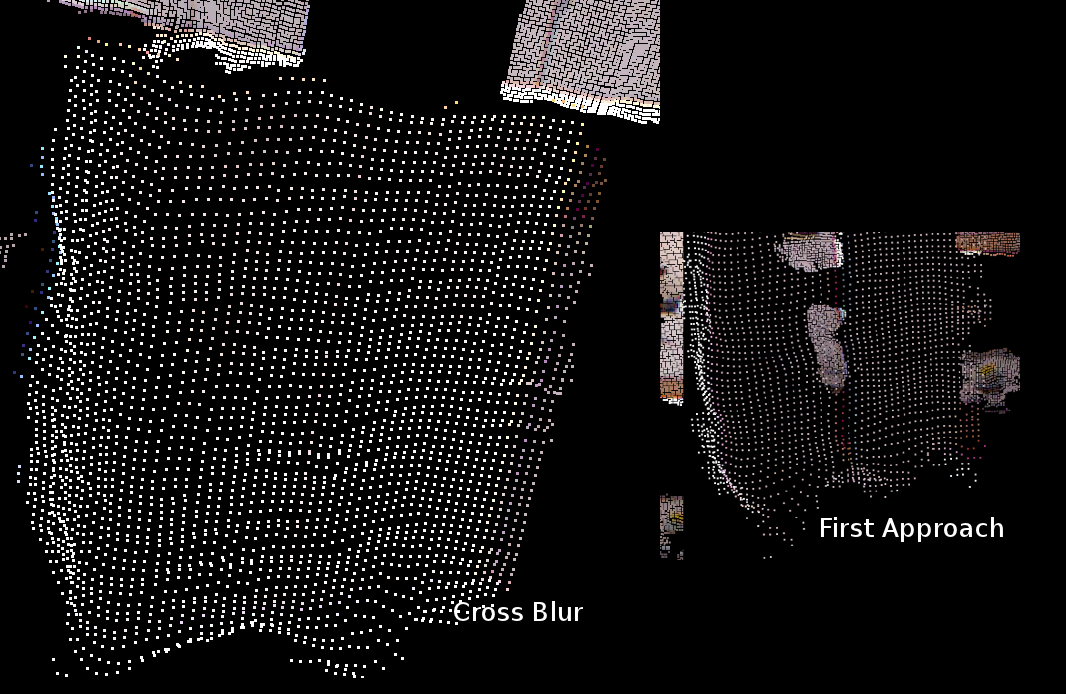
\includegraphics[width=\textwidth]{crossBlurResult.png}
  \caption{Cross Blur Result}
  \label{figure:crossblurResult}
\end{center}
\end{figure} 


\subsection{Calculation of X and Y Distance}
After bluring the depth, the real world X and Y values of each point must be calculated. 
This is done with the camera information delivered from ROS in the camera\_info message.
The message contains information of the camera intrinsics, including the focal 
distances for the x- and y-axis which are needed here.

The X and Y values are calculated by equations \vref{eq:X} and \vref{eq:Y} where $center_x$ and $center_y$ are
the coordinates of the image center and $f_x$ and $f_y$ the focal distances in x- and y-direction. As in the
previous sections $D$ represents the value of a pixel in the depth image.

\begin{equation}
X(x,y)=\frac{(x-center_x) \cdot D(x,y)}{f_x}
\label{eq:X}
\end{equation}

\begin{equation}
Y(x,y)=\frac{(y-center_y) \cdot D(x,y)}{f_y}
\label{eq:Y}
\end{equation}

The code for this is mostly copied from the rgbxyz-point cloud nodelet from ROS with a few changes.
All of the float values are multiplied by 100 and converted to integer. This is used to increase the accuracy while
calculating a integer value for x and y coordinates. The coordinates itself are stored as short. This was done to save
computational time by calculating the normals with short instead of the double format.

The full code of the function to create the XY-map is shown in the listing \vref{lst:xymap}.
\begin{lstlisting}[caption={createXYMap - Function\label{lst:xymap}},language=C++]
void createXYMap(const cv::Mat &src, 
				 const sensor_msgs::CameraInfoConstPtr& info_msg, 
				 cv::Mat &xy)
{
	if(src.type() == CV_16UC1)
	{
		xy=cv::Mat::zeros(src.rows,src.cols,CV_16UC2);

		image_geometry::PinholeCameraModel model;
		model.fromCameraInfo(info_msg);

		int center_x = model.cx()*100;	
		int center_y = model.cy()*100;

		int constant_x = model.fx()*100;
		int constant_y = model.fy()*100;

		int size_x=src.cols, size_y=src.rows;

		int x,y;
		for (int i = 0; i < (size_x*size_y); i++)
		{
			y=i/size_x;
			x=i-y*size_x;

			if(x>0)
			{
				short depth=src.at<Vec1shrt>(y,x)[0];
				xy.at<Vec2shrt>(y,x)[0] = ((x*100 - center_x) * depth) / constant_x;
				xy.at<Vec2shrt>(y,x)[1] = ((y*100 - center_y) * depth) / constant_y;
			}
		}
	}
	else
	{
		ROS_ERROR("WRONG TYPE: createXYMap");
	}
}
\end{lstlisting}


\subsection{3D RangeFilter}
When the real X and Y values for each pixel are known, it is possible to clear pixels in the output depth image $D_{out}$ 
by setting minimum and maximum values for all axis.


\begin{equation}
	\begin{split}
	   (X < Xmin \vee X > Xmax \vee Y > Ymax \vee Y < Ymin \vee D(x,y) < Zmin \vee D(x,y) > Zmax)\\
	   \implies D_{out}(x,y) = 0
   \end{split}
\end{equation}

Listing \vref{lst:range3d} shows the code of the 3D Range Filter and figure \vref{figure:xyzrange} the working principle.

\begin{lstlisting}[caption={XYZrangeFilter - Function\label{lst:range3d}},language=C++]
void XYZrangeFilter(const cv::Mat &depth, 
                    const cv::Mat &xy, 
                    cv::Mat &depth_out, 
                    int min_x, int max_x, 
                    int min_y, int max_y, 
                    int min_z, int max_z)
{

	int size_x=depth.cols, size_y=depth.rows;
	depth_out=depth.clone();
	int y,x;
	for (int i = 0; i < (size_x*size_y); i++)
	{
		y=i/size_x;
		x=i-y*size_x;


		short cur_z=depth_out.at<Vec1shrt>(y,x)[0];


		if(cur_z == 0) continue; //If depth == 0 continue with next pixel

		int cur_x=xy.at<Vec2shrt>(y,x)[0];
		int cur_y=xy.at<Vec2shrt>(y,x)[1];

		if(!((cur_x >= min_x && cur_x <= max_x)&&
		     (cur_y >= min_y && cur_y <= max_y)&&
		     (cur_z >= min_z && cur_z <= max_z)))
		{
			depth_out.at<Vec1shrt>(y,x)[0]=0;
		}
	}
}
\end{lstlisting}


\begin{figure}[H]
\begin{center}
  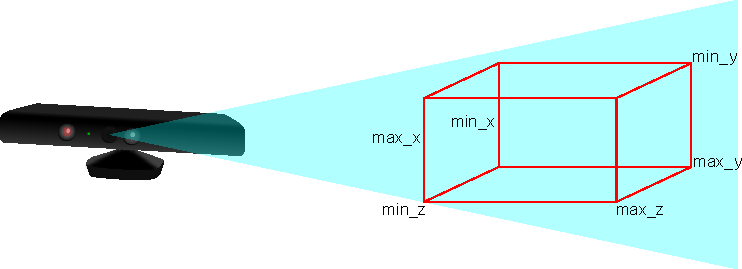
\includegraphics[width=\textwidth]{XYZFilter.pdf}
  \caption{XYZ-Range-Filter Concept}
  \label{figure:xyzrange}
\end{center}
\end{figure}


\subsection{Normal Calculation}
With the depth image and the xy map the normal of each pixel can be calculated. This is done by the scalar product
shown in figure \vref{eq:scalar}.

\begin{equation}
 \vec{N} =        \left( \begin{array}{c} x_u                           \\                           y_u \\ z_u                           \end{array} \right) 
           \times \left( \begin{array}{c} x_v                           \\                           y_v \\ z_v                           \end{array} \right) 
         =        \left( \begin{array}{c} y_u \cdot z_v - z_u \cdot y_v \\ z_u \cdot x_v - z_v \cdot x_u \\ x_u \cdot y_v - y_u \cdot x_v \end{array}\right)
\label{eq:scalar}
\end{equation}


The current algorithm tries to calculate two normals, one calculated with the vector from the current pixel to the top and right 
($\vec{N}_{tr}=\vec{V_t}\times\vec{V_r}$) and one to the bottom and left ($\vec{N_{bl}}=\vec{V_b}\times\vec{V_l}$). To check
if the vectors can be calculated, the data from the neighborhood map is used, so the values from equation 
\vref{eq:neighbors_bit} are needed again for equations \vref{eq:vec_tr} and \vref{eq:vec_bl}. 


\begin{gather}
 \vec{N}_{tr}(x,y)=    \vec{V}_t(x,y) \times \vec{V}_r(x,y) =
                  \left( \begin{array}{c}   X(x,y-1) -  X(x,y)  \\ Y(x,y-1) -  Y(x,y) \\ D(x,y-1) -  D(x,y)\end{array} \right) 
           \times \left( \begin{array}{c}   X(x+1,y) -  X(x,y)  \\ Y(x+1,y) -  Y(x,y) \\ D(x+1,y) -  D(x,y)\end{array} \right)\nonumber
			\\\mbox{(When $b_1(x,y)=true$ and $b_3(x,y)=true$)}
\label{eq:vec_tr}\\
 \vec{N}_{bl}(x,y)=    \vec{V}_b(x,y) \times \vec{V}_l(x,y) =
                  \left( \begin{array}{c}   X(x,y+1) -  X(x,y)  \\ Y(x,y+1) -  Y(x,y) \\ D(x,y+1) -  D(x,y)\end{array} \right) 
           \times \left( \begin{array}{c}   X(x-1,y) -  X(x,y)  \\ Y(x-1,y) -  Y(x,y) \\ D(x-1,y) -  D(x,y)\end{array} \right)\nonumber
			\\\mbox{(When $b_5(x,y)=true$ and $b_7(x,y)=true$)}
\label{eq:vec_bl}
\end{gather}

If both normals can be calculated it takes the average of both normals (see figure \vref{figure:normals}) with equation 
\vref{eq:vec_avg}.

\begin{gather}
	\vec{N}(x,y) = \frac{\vec{N}_{tr}(x,y) + \vec{N}_{bl}(x,y)}{2}\nonumber\\
\mbox{\hspace{0.5cm}(When $b_1(x,y)=true$, $b_3(x,y)=true$, $b_5(x,y)=true$ and $b_7(x,y)=true$)}
\label{eq:vec_avg} 
\end{gather} 


\begin{figure}[H]
\begin{center}
  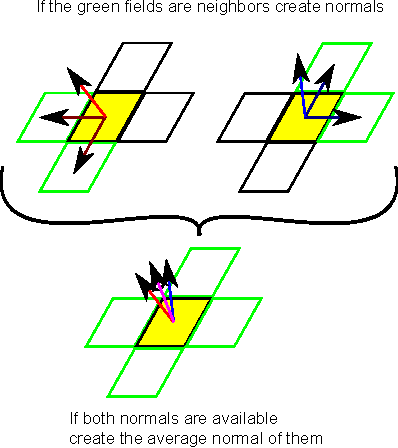
\includegraphics[width=\textwidth/3]{normals.pdf}
  \caption{Normals Creation}
  \label{figure:normals}
\end{center}
\end{figure}

\subsection{Angle Calculation}

The angles from vectors to the axes are basically calculated by the equations \ref{eq:angle_a}, \ref{eq:angle_b} and
\vref{eq:angle_g}. Where $\alpha$, $\beta$ and $\gamma$ are the angles to the x,y, and z-axis 
of the normal vector $\vec{N}$ as seen in figure \vref{figure:NormalAngles}.

\begin{figure}[H]
\begin{center}
  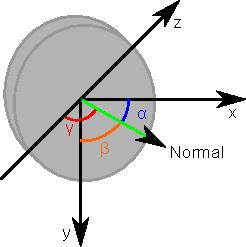
\includegraphics[width=\textwidth/3]{Angles.pdf}
  \caption{Angles of a Normal}
  \label{figure:NormalAngles}
\end{center} 
\end{figure}

\begin{align}
 \alpha = \arccos \frac{N_x}{\left|\vec{N}\right|}  
\label{eq:angle_a}\\
 \gamma = \arccos \frac{N_z}{\left|\vec{N}\right|}  
\label{eq:angle_b}\\
 \beta  = \arccos \frac{N_y}{\left|\vec{N}\right|}  
\label{eq:angle_g}
\end{align}


In the application the arcus cosinus values are precalculated to save computational time.
The possible input range for the arcus cosinus function lies between -1 and 1, so it was decided
to precalculate 2000 values for the lookup table. This means the possible input values are now
-1000 to 1000. To bring them into the possible range 1000 needs to be added to all input values.
The precalulated values also include the transformation from radian to degree and are stored as 
integer values which were multiplied by 100 to save two digits behind the comma.

So the precalculation for the values in the arcus cosinus look-up table $acos(k)$ 
in the array, are done with equation \vref{eq:acos_precalc}.

\begin{equation}
	pacos(k)=\lfloor \arccos ((k-1000)/1000) * \frac{180}{\pi}*100 + 0,5 \rfloor
	\mbox{\hspace{0.5cm} (Where 0<=k<=2000)}
	\label{eq:acos_precalc}
\end{equation}

To obtain the values from the array, the result of the devision from a vector part through its length
must be multiplied with 1000 and added to 1000. To be able to display the angles easily for debuging 
it was later decided to put the values in a matrix for an RGB image, so each value has to be devided 
by 100 again because unsigned char only supports values from 0 to 255.

For one vector in the normal map $\vec{N}(x,y)$ this results in the equations \ref{eq:angleX}, \ref{eq:angleY} and
\vref{eq:angleZ} for the array index k.

\begin{align}
	k_\alpha(x,y) = \left\lfloor\frac{N_X(x,y)*1000}{\sqrt{N_X(x,y)^2+N_Y(x,y)^2+N_Z(x,y)^2}}+1000 \right\rfloor
	\label{eq:angleX}\\
	k_\beta(x,y) = \left\lfloor\frac{N_Y(x,y)*1000}{\sqrt{N_X(x,y)^2+N_Y(x,y)^2+N_Z(x,y)^2}}+1000 \right\rfloor
	\label{eq:angleY}\\
	k_\gamma(x,y) = \left\lfloor\frac{N_Z(x,y)*1000}{\sqrt{N_X(x,y)^2+N_Y(x,y)^2+N_Z(x,y)^2}}+1000 \right\rfloor
	\label{eq:angleZ}
\end{align} 

With the values for k, the angles can be gathered from the look-up table resulting in the final equations \ref{eq:anglePX},
\ref{eq:anglePY} and \vref{eq:anglePZ}.

\begin{align}
	\alpha(x,y)=\frac{pacos({k_\alpha(x,y)})}{100}\label{eq:anglePX}\\
	\beta(x,y)=\frac{pacos({k_\beta(x,y)})}{100}\label{eq:anglePY}\\
	\gamma(x,y)=\frac{pacos({k_\gamma(x,y)})}{100}\label{eq:anglePZ}	
\end{align}



The following listing \vref{lst:AngleMap} shows the code for the angle calculation function.

\begin{lstlisting}[caption={createAngleMap - Function}\label{lst:AngleMap},language=c++]
void createAngleMap(const cv::Mat &normals, cv::Mat &angles)
{
	angles=cv::Mat::zeros(normals.rows,normals.cols,CV_8UC3);
	int size_x=normals.cols, size_y=normals.rows;
	int y,x;
	for (int i = 0; i < (size_x*size_y); i++)
	{ 
		y=i/size_x;
		x=i-y*size_x;

		short g1=(normals.at<Vec3shrt>(y,x)[0]);
		short g2=(normals.at<Vec3shrt>(y,x)[1]);
		short g3=(normals.at<Vec3shrt>(y,x)[2]);

		double vector_length=sqrt(g1*g1+g2*g2+g3*g3);
		if(!vector_length)continue;

		angles.at<Vec3uchar>(y,x)[0]=preCalcCos[(int)(g1*1000/vector_length)+1000]/100;
		angles.at<Vec3uchar>(y,x)[1]=preCalcCos[(int)(g2*1000/vector_length)+1000]/100;
		angles.at<Vec3uchar>(y,x)[2]=preCalcCos[(int)(g3*1000/vector_length)+1000]/100;
	}
}	
\end{lstlisting}

\subsection{Angle Bluring}

To blur the angles the same method as mentioned in chapter \vref{sect:blurFilter} was used and
but the average is done for each angle seperately. The comparison between a blured and a non-blured
angle picture is shown in figure \vref{figure:AnglesBlured}.

\begin{figure}[H]
\begin{center}
  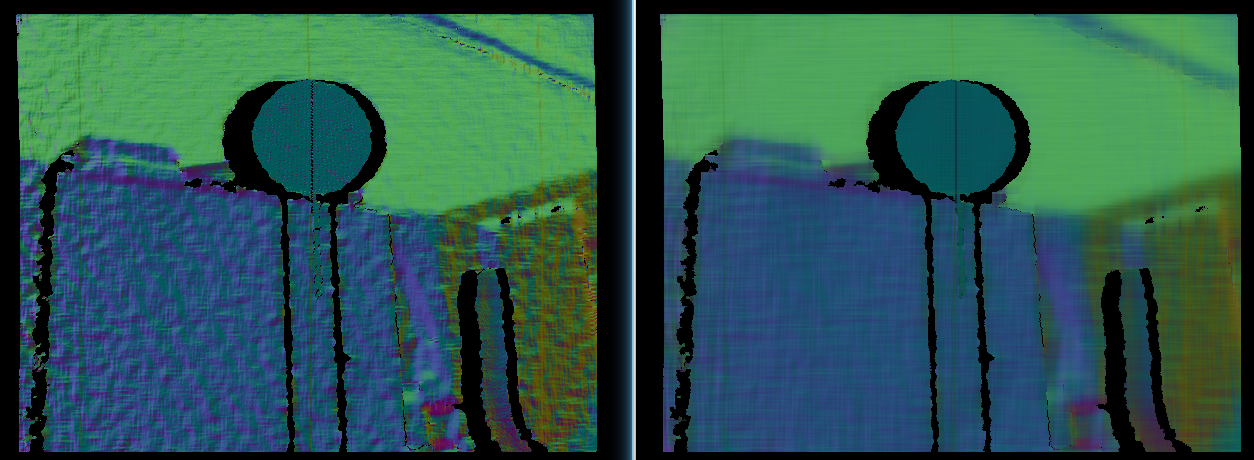
\includegraphics[width=\textwidth]{AnglesMapBlured.png}
  \caption{Angles Map non-blured and blured}
  \label{figure:AnglesBlured}
\end{center}
\end{figure}


\subsection{Angle Filtering}

To get only surfaces which are interesting, a angle filter was created. It's input parameters
are the minimum and maxium for each angle. The output of this function is a grayscale image
where pixels all $P_{ok}$ are initialized with 0 and those with suitable angles get the value 255
(as seen in equation \vref{eq:anglefilter}).

\begin{gather}
(min\_\alpha  <= \alpha(x,y) <=max\_\alpha ) \wedge \nonumber\\ 
(min\_\beta  <= \beta(x,y) <=max\_\beta )\wedge\nonumber\\
(min\_\gamma  <= \gamma(x,y) <=max\_\gamma )\nonumber\\
\implies P_{ok}(x,y) = 255;
\label{eq:anglefilter}
\end{gather}

The function also features another mode, where the output image contains the suitable angles instead of only 255.
But this mode is not used in the project. 

\subsection{Surface Segmentation}

Before begining with segmenting the surfaces, the picture containing the pixels showing 
correct angles is blured with an aperture of $5 \times 5$ to remove empty pixels or columns of empty pixels 
which seperate surfaces belonging together. After bluring them, the threshold function is used to bring 
all pixels, which are not zero, to the value 255 (see equation \vref{eq:thresholdSeg}).
The code for the C++ function is shown in listing \vref{lst:blurAthres}.

\begin{lstlisting}[caption={Bluring and Thresholding}\label{lst:blurAthres},language=c++]
	cv::blur(angles_ok,angles_ok,cv::Size(5,5),cv::Point(-1,-1),0);
	cv::threshold(angles_ok,angles_ok,1,255,0);
\end{lstlisting}

\begin{equation}
	P_{ok}(x,y)>=1 \implies P_{ok}(x,y)=255
	\label{eq:thresholdSeg}
\end{equation}


The segmentation algorithm uses a class named $range$ to outline pixel blobs in regions. The class contains integer 
variables for the minimal and maximal x and y values. All created $range$ objects are stored inside  
a std::vector at the index which has the same number as the ID they belong to. 
The algorithm seeks for pixels which are not zero in the $P_{ok}$-image and have neighbors.

If it finds one, it starts to look, if there is neighbor at the pixels top($b_1$), top-left($b_0$), 
left($b_7$) and bottom-left($b_6$) ($b_i$ from equation \vref{eq:neighbors_bit} is used here again).
If it finds a pixel, which is a neighbor and has an suitable angle, then it gathers its ID in the IDs matrix, 
sets the current pixel $P_{id}(x,y)$ in the ID matrix to this ID and calls the update function of the corresponding 
range object in the vector which updates minimum and maximum values. After that, it checks 
if the rest of the pixels, not checked in step one, are neighbors and have suitable angles. 
If it finds one, which has a different ID, it creates a relation between 
them inside a std::set, a special form of a container, which allows only unique items. 
If this is done for each of the remaining 
neighbors, the algorithm advances to the next pixel. If a pixel contains neighbors, but doesn't have a neighbor at the locations
mentioned before, a new ID and a range object are created. The range objects minimum and maximum x and y are initialized 
to the values of the current pixel. This part of the algorithm is shown in algorithm \vref{alg:IDs} 
and visualized in figure \vref{figure:segment}.

\begin{algorithm}[H]

	\begin{algorithmic}
\ForAll{x,y} 
	\State {$b_t  \gets b_1(x,y) $}
	\State {$b_tl \gets b_0(x,y) $}
	\State {$b_l  \gets b_7(x,y) $}
	\State {$b_bl \gets b_6(x,y) $}
	\State {$p  \gets 0$}
	\State {$last_id \gets 0$}
	
		\If{$b_t=true \wedge P_{id}(x,y-1)\neq 0 \wedge P_{ok}(x,y-1)$}
				\State {$P_{id}(x,y) \gets P_{id}(x,y-1)$}
				\State {$p \gets 1$}
				\State {Call $ranges[P_{id}(x,y)].update(x,y)$}
		\ElsIf{$b_tl=true \wedge P_{id}(x-1,y-1)\neq 0 \wedge P_{ok}(x-1,y-1)$}
				\State {$P_{id}(x,y) \gets P_{id}(x-1,y-1)$}
				\State {$p \gets 2$}
				\State {Call $ranges[P_{id}(x,y)].update(x,y)$}
		\ElsIf{$b_l=true \wedge P_{id}(x-1,y)\neq 0 \wedge P_{ok}(x-1,y)$}
				\State {$P_{id}(x,y) \gets P_{id}(x-1,y)$}
				\State {$p \gets 3$}
				\State {Call $ranges[P_{id}(x,y)].update(x,y)$}
		\ElsIf{$b_bl=true \wedge P_{id}(x-1,y+1)\neq 0 \wedge P_{ok}(x-1,y+1)$}
				\State {$P_{id}(x,y) \gets P_{id}(x-1,y+1)$}
				\State {$p \gets 4$}
				\State {Call $ranges[P_{id}(x,y)].update(x,y)$}
		\Else
				\State {$lastID \gets last_ID+1$}
				\State {$ranges[lastID] \gets $ new range object}
				\State {$P_{id}(x,y) \gets lastID$}
				\State {$p \gets 5$}
		\EndIf
		
		\If{$b_tl=true \wedge p<1 \wedge P_{id}(x-1,y-1) \neq P_{id}(x,y)$}
			\State{$relations.insert(P_{id}(x,y), P_{id}(x-1,y-1))$}
		\EndIf
		
		\If{$b_l=true \wedge p<2 \wedge P_{id}(x-1,y) \neq P_{id}(x,y)$}
			\State{$relations.insert(P_{id}(x,y), P_{id}(x-1,y-1))$}
		\EndIf
		
		\If{$b_bl=true \wedge p<3 \wedge P_{id}(x-1,y+1) \neq P_{id}(x,y)$}
			\State{$relations.insert(P_{id}(x,y), P_{id}(x-1,y-1))$}
		\EndIf
\EndFor
	\end{algorithmic}
 \caption{Segmentation: ID Assignment}
 \label{alg:IDs}
\end{algorithm}


\begin{figure}[H]
\begin{center}
  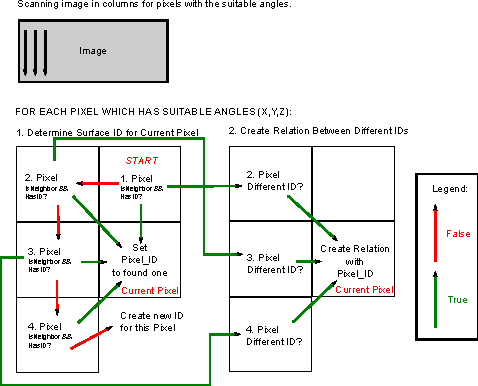
\includegraphics[width=\textwidth]{SurfaceSegmentation.pdf}
  \caption{Segmentation: Getting ID - Creating Relations}
  \label{figure:segment}
\end{center}
\end{figure}

After passing the whole neighborhood-map, all range objects having a relation are merged together
by a loop executing the merge function of one range class object with the relating one.
The merge function first calls the getLast function of both objects, which returns a pointer to the
last range objects, the ranges were merged to, then those objects are merged together. 
This is necessary to merge all objects together recursively. At the end, the regions of the range objects are 
filtered by size and stored in the output array for template matching. 

\definecolor{darkgreen}{RGB}{0,128,0}
How this works is shown in figure \vref{figure:Merging}, where all ranges belong to one blob. For the range objects
the following relations exist: 1-2, 3-4, \textcolor{red}{2-4}, 5-6 and \textcolor{darkgreen}{1-6}.

\begin{figure}[H]
\begin{center}
  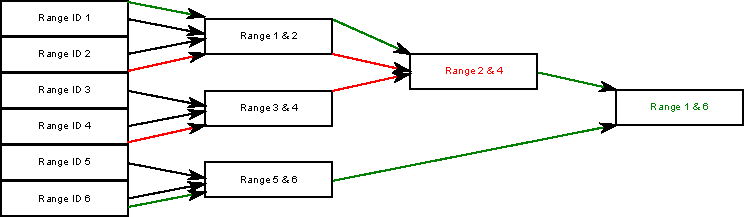
\includegraphics[width=\textwidth]{merging.pdf}
  \caption{Segmentation: Merging Range Objects}
  \label{figure:Merging}
\end{center}
\end{figure}
 



\begin{figure}[H]
\begin{center}
  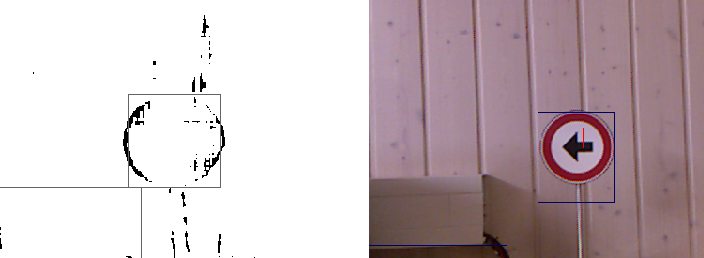
\includegraphics[width=\textwidth]{AnglesOkSegment.png}
  \caption[Angles OK Image and RGB Picture]{Angles OK image and RGB Picture\footnotemark}
  \label{figure:AnglesOKSeg}
\end{center}
\end{figure}
\footnotetext{Camera was held with hands thus pictures are not from the same distance and angle}
\newpage

\section{RGB Image Processing}

When all surface regions have been determined, it's time to start with fitting the RGB image 
to the right perspective to search for patterns in the regions. 


\section{Warping Prespective}
For adjusting the perspective from a surface in the RGB image the OpenCV function warpPerspective
 is used comination with getPerspectiveTransform.
``\textit{
getPerspectiveTransform calculates the perspective transform from 4 pairs of the corresponding points. The function 
calculates the $3 \times 3$ matrix of a perspective transform such that:
\begin{gather}
\begin{bmatrix} t_i x'_i \\ t_i y'_i \\ t_i \end{bmatrix} = \texttt{map\_matrix} \cdot \begin{bmatrix} x_i \\ y_i \\ 1 \end{bmatrix} 
\nonumber\\\mbox{where}\nonumber\\dst(i)=(x'_i,y'_i), src(i)=(x_i, y_i), i=0,1,2 
\end{gather}
}''
\cite{willowgarage:opencv:getPerspectiveTransform}.

``\textit{
The function warpPerspective applies a perspective transformation to the source image using the specified matrix:
\begin{gather}
\texttt{dst} (x,y) = \texttt{src} \left ( \frac{M_{11} x + M_{12} y + M_{13}}{M_{31} x + M_{32} y + M_{33}} , \frac{M_{21} x + M_{22} y + M_{23}}{M_{31} x + M_{32} y + M_{33}} \right ) 
\end{gather}
}''
\cite{willowgarage:opencv:warpPerspective} 

For calculating the points, it is necessary to pick four points arranged in a quadrat with a side length of $s$
(top-left $(x_{tl},y_{tl})$,top-right $(x_{tr},y_{tr})$, bottom-left $(x_{bl},y_{bl})$  and bottom-right point $(x_{br},y_{br})$) 
from the surface. 
After picking them, the real coordinates $X$, $Y$ and $Z$ ($D$) are obtained to calculate 
the real distances between the corresponding points ($d_{top}$, $d_{left}$, $d_{right}$, $d_{bottom}$)
(see equations \ref{eq:distT}, \ref{eq:distR}, \ref{eq:distB} and \vref{eq:distL}).
The distances are needed calculate the new proportions for the coordinates of the pixels in the RGB image, so that
the texture will be streched to the real proportions to do template matching. Normally this would be done like in
part a) of figure \vref{figure:perspective}, by scaling the smaller side to the bigger and then matching the proportions
of height and width. In software this is done with the method shown in part b). 
The lower point of the smaller side is shifted down by the full difference of the sides, while at the other, 
the bigger side, both points are moved down by the half of it. When calculating the new point coordinates,
always the smaller side is scaled to the bigger, that's why there are two different ways mentioned to 
calculate the new coordinates. At the end, it is necessary to bring both sides to the same length
(see equations \ref{eq:points_qv} to \vref{eq:points_br_x_2}). Figure \vref{figure:perspectiveResult}
shows the input and output of warpPerspective. 



{
\footnotesize
\begin{align}
	d_{top}=\sqrt{(X_{tl}(x_{tl},y_{tl})-X_{tr}(x_{tr},y_{tr}))^2+(Y_{tl}(x_{tl},y_{tl})-Y_{tr}(x_{tr},y_{tr}))^2+(Z_{tl}(x_{tl},y_{tl})-Z_{tr}(x_{tr},y_{tr}))^2}\label{eq:distT}\\
	d_{right}=\sqrt{(X_{br}(x_{br},y_{br})-X_{tr}(x_{tr},y_{tr}))^2+(Y_{br}(x_{br},y_{br})-Y_{tr}(x_{tr},y_{tr}))^2+(Z_{br}(x_{br},y_{br})-Z_{tr}(x_{tr},y_{tr}))^2}\label{eq:distR}\\
	d_{bottom}=\sqrt{(X_{bl}(x_{bl},y_{bl})-X_{br}(x_{br},y_{br}))^2+(Y_{bl}(x_{bl},y_{bl})-Y_{br}(x_{br},y_{br}))^2+(Z_{bl}(x_{bl},y_{bl})-Z_{br}(x_{br},y_{br}))^2}\label{eq:distB}\\
	d_{left}=\sqrt{(X_{tl}(x_{tl},y_{tl})-X_{bl}(x_{bl},y_{bl}))^2+(Y_{tl}(x_{tl},y_{tl})-Y_{bl}(x_{bl},y_{bl}))^2+(Z_{tl}(x_{tl},y_{tl})-Z_{bl}(x_{bl},y_{bl}))^2}\label{eq:distL}
\end{align}
}
\newpage
\begin{align}
 q_v = \left\{ 
	 \begin{array}{ll}
	 {d_{right}}/{d_{left}} &\mbox{\hspace{0.5cm}} d_{left}<d_{right}\\
	 {d_{left}}/{d_{right}} &\mbox{\hspace{0.5cm}} otherwise
	 \end{array} 
\right.\label{eq:points_qv}\\
y_{tr}=\left\{ 
	 \begin{array}{ll}
	 {y_{tr} + \frac{s\cdot q}{2}} &\mbox{\hspace{0.5cm}} d_{left}<d_{right}\\
	 {y_{tr}} &\mbox{\hspace{0.5cm}} otherwise
	 \end{array}\right.\label{eq:points_tr_y}\\
y_{br}=\left\{ 
	 \begin{array}{ll}
	 {y_{br} + \frac{s\cdot q}{2}} &\mbox{\hspace{0.5cm}} d_{left}<d_{right}\\
	 {y_{br}} &\mbox{\hspace{0.5cm}} otherwise
	 \end{array}\right.\label{eq:points_br_y}\\
y_{tl}=\left\{ 
	 \begin{array}{ll}
	 {y_{tl}} &\mbox{\hspace{0.5cm}} d_{left}<d_{right}\\
	 {y_{tl} + \frac{s\cdot q}{2}} &\mbox{\hspace{0.5cm}} otherwise
	 \end{array}\right.\label{eq:points_tl_y}\\
y_{bl}=\left\{ 
	 \begin{array}{ll}
	 {y_{bl}} &\mbox{\hspace{0.5cm}} d_{left}<d_{right}\\
	 {y_{bl} + \frac{s\cdot q}{2}} &\mbox{\hspace{0.5cm}} otherwise
	 \end{array}\right.\label{eq:points_bl_y}\\
b_v    =\left\{ 
	 \begin{array}{ll}
	 d_{right} &d_{left}<d_{right}\\
	 d_{left} &\mbox{\hspace{0.5cm}} otherwise
	 \end{array}\right.\label{eq:points_bv}\\
q_h = \left\{ 
	 \begin{array}{ll}
	 {d_{top}}/{d_{bottom}} &\mbox{\hspace{0.5cm}} d_{bottom}<d_{top}\\
	 {d_{bottom}}/{d_{top}} &\mbox{\hspace{0.5cm}} otherwise
	 \end{array} 
\right.\label{eq:points_qh}\\
x_{br}=\left\{ 
	 \begin{array}{ll}
	 {x_{br} + \frac{s\cdot q_h}{2}} &\mbox{\hspace{0.5cm}} d_{bottom}<d_{top}\\
	 {x_{br}} + s &\mbox{\hspace{0.5cm}} otherwise
	 \end{array}\right.\label{eq:points_br_x}\\
x_{bl}=\left\{ 
	 \begin{array}{ll}
	 {x_{bl} + \frac{s\cdot q_h}{2}} &\mbox{\hspace{0.5cm}} d_{bottom}<d_{top}\\
	 {x_{bl}} &\mbox{\hspace{0.5cm}} otherwise
	 \end{array}\right.\label{eq:points_bl_x}\\
x_{tr}=\left\{ 
	 \begin{array}{ll}
	 {x_{tr}} + s &\mbox{\hspace{0.5cm}} d_{bottom}<d_{top}\\
	 {x_{tr} + \frac{s\cdot q_h}{2}} &\mbox{\hspace{0.5cm}} otherwise
	 \end{array}\right.\label{eq:points_tr_x}\\
x_{tl}=\left\{ 
	 \begin{array}{ll}
	 {x_{tl}} &\mbox{\hspace{0.5cm}} d_{bottom}<d_{top}\\
	 {x_{tl} + \frac{s\cdot q_h}{2}} &\mbox{\hspace{0.5cm}} otherwise
	 \end{array}\right.\label{eq:points_tl_x}\\
b_h    =\left\{ 
	 \begin{array}{ll}
	 d_{top} &d_{bottom}<d_{top}\\
	 d_{bottom} &\mbox{\hspace{0.5cm}} otherwise
	 \end{array}\right.\label{eq:points_bh}\\
 x_{tr} = x_{tr} + s \cdot \frac{d_{left}}{d_{top}} - s\label{eq:points_tr_x_2}\\
 x_{br} = x_{br} + s \cdot \frac{d_{left}}{d_{top}} - s\label{eq:points_br_x_2}
\end{align}  

\begin{figure}[H]
\begin{center}
  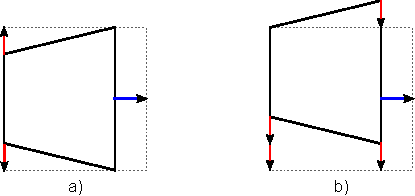
\includegraphics[width=\textwidth]{PerspectiveTransform.pdf}
  \caption[]{Perspective Transform}
  \label{figure:perspective}
\end{center}
\end{figure}

\begin{figure}[htp]
\begin{center}
  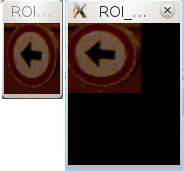
\includegraphics[width=\textwidth/2]{warpPerspective.png}
  \caption{Result of a Perspective Transform (Input and Output)}
  \label{figure:perspectiveResult}
\end{center}
\end{figure}


\subsection{First template matching approach}
The first approach on finding the signs was done with a HSV color filter and the hough transformation
function from OpenCV, which finds circle in an image or a given region of an image.

The color filter must be in HSV because with that color scheme, it is possible to filter for colors
with the H(hue) part of the pixel. In figure \vref{figure:hsv} the green boxes define the color range
which is interesting. Every pixel with another color will be set to zero. 

\begin{figure}[htp]
\begin{center}
  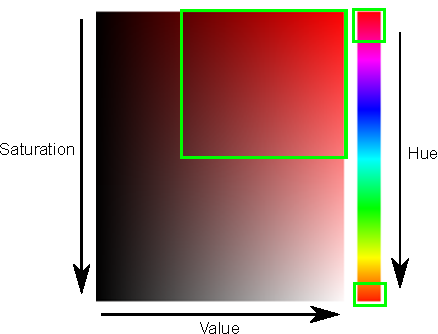
\includegraphics[width=\textwidth]{HSV.pdf}
  \caption{HSV Color Range}
  \label{figure:hsv}
\end{center}
\end{figure}


\begin{figure}[htp]
\begin{center}
  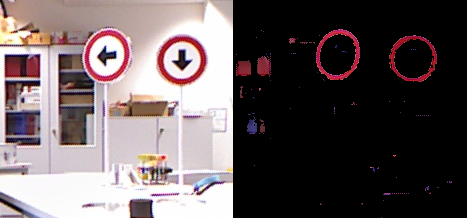
\includegraphics[width=\textwidth]{redFilterResult.png}
  \caption{Result of the HSV based Red Filter}
  \label{figure:redFilter}
\end{center}
\end{figure}


For a result picture see figure \vref{figure:redFilter}. 
Only the circles and some other red objects are visible. 
The next step is transfering the image to grayscale and 
bluring the image. After that a hugh transformation is done which will gather round
objects in the picture. If a circle is found a the template is scaled to it's size and 
searched in a region a bit bigger than the found circle. This will most likely bring some good results, 
but in many cases the inner circle is found instead of the outer one, and when that happens the image 
differences are mostly too small to determine that it is a wrong match
(see example in figure \vref{figure:problemCircles}).

\begin{figure}[H]
\begin{center}
  
\includegraphics[width=\textwidth/2]{robotSignProblem.pdf}
  \caption{Problem with to small circle sizes}
  \label{figure:problemCircles}
\end{center}
\end{figure}

\subsection{Proportion Enhanced Template Matching}
To optimize the template matching another way was found. This algorithm
takes the template picture and converts it to grayscale. It starts at the top-left pixel
and searches for the first non translucent pixel diagonally. If it has found it,
it determines if the pixel is dark (value <= 127) or light (value>127). Then it
starts to seek for the next change, when the value passes 127 again.
When it changes, the alogrithm gathers the distance from pixel to pixel and searches for the next change.
When that change appears, it calculates the proportion of both lengths and stores it 
with the location of the current pixel and the length from the first change to the endpoint. 
The proportion will be negative, if pixels are changing to dark, to prevent finding negatives of the template. 
This is now done as long as the algorithm reaches an edge of the template 
(for an Example see in figure \vref{figure:templateProp}).

\begin{figure}[H]
\begin{center}
  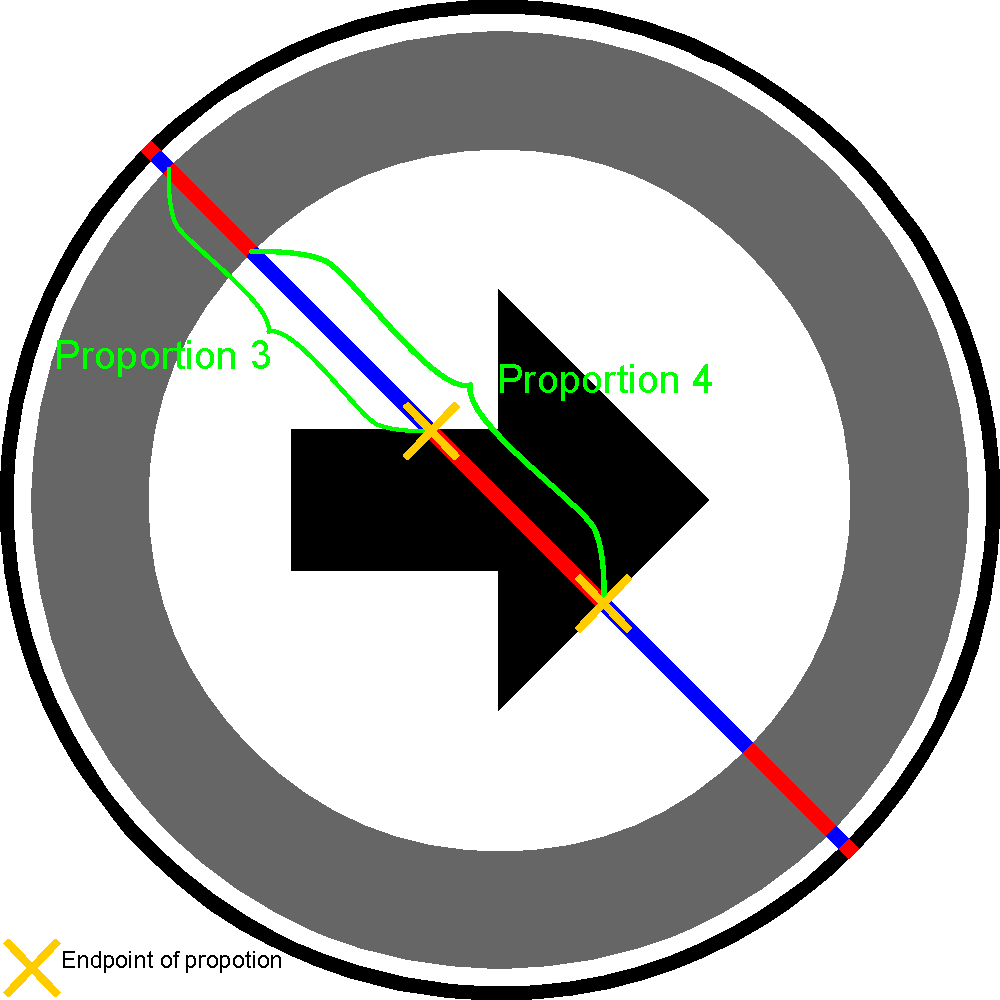
\includegraphics[width=\textwidth/2]{proportionGather.pdf}
  \caption{Gathering Proportions in Template}
  \label{figure:templateProp}
\end{center}
\end{figure}

In the next step the algorithm searches the target picture with the same method, but
it doesn't only search the diagonal row beginning in the top left corner, it searches
through the whole picture. To prevent problems with the lightning, the threshhold
for searching the picture ($th_{target}$) is automatically determined by half of the sum of the 
minimum ($g_{min}$) and maximum grayscale value($g_{max}$) of all image pixels
as seen in equation \vref{eq:autothres}.

	\begin{equation}
		th_{target}=\frac{g_{max}+g_{min}}{2}
		\label{eq:autothres}
	\end{equation}

Always when it has found two consecutive pixel strings it creates the proportion. 
Then it calls a method of the objects the templates are stored in.
This method takes each proportion and checks if this proportion is available for
the current template. If it is, it is stored inside a pair. If a pair of two
consecutive proportions is found, it takes the distance length of the last
proportion in the target picture and devides it by the length of the matching proportion
in the template. 

The resulting factor is used to scale the template to the size of the
proportion in the picture and to determine the new point of the proportion in the scaled template.
With this point, the position, for trying to match the template, is calculated 
(see in figure \vref{figure:findPropTempPlace}).

\begin{figure}[H]
\begin{center}
  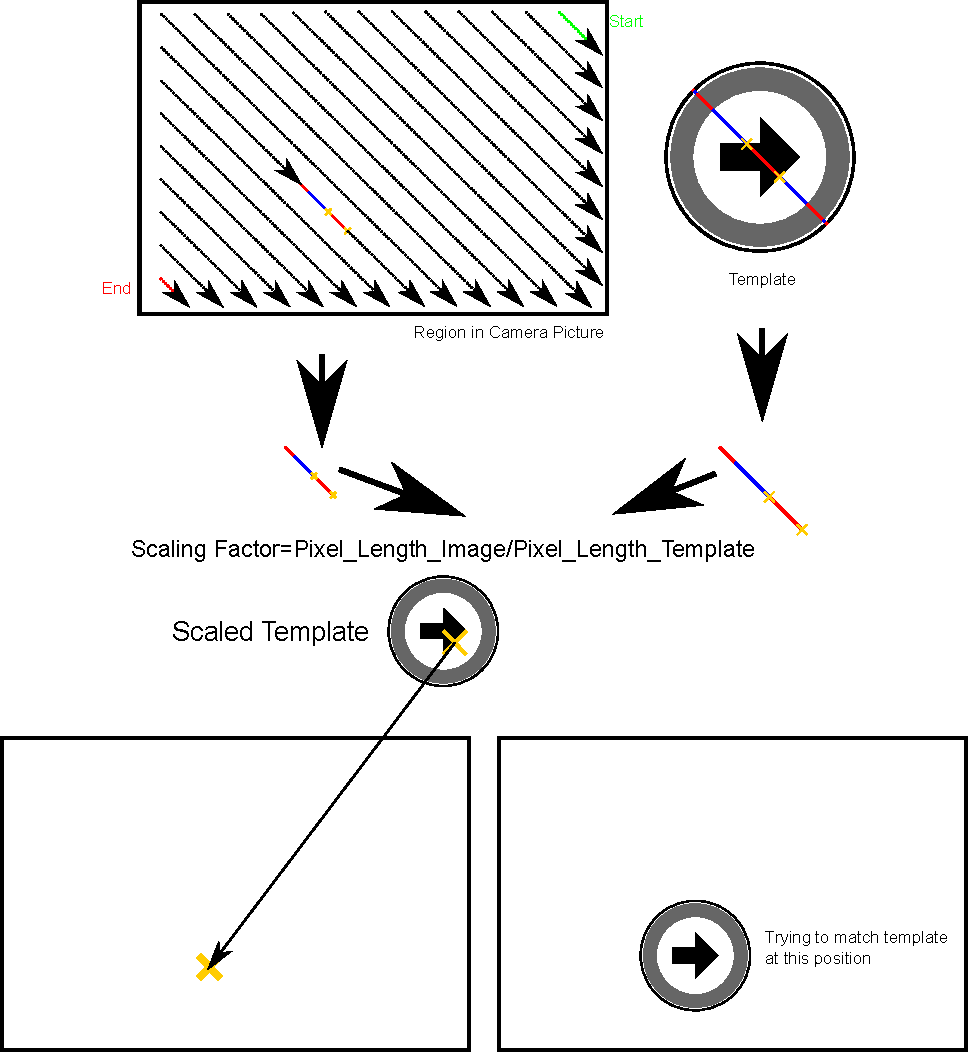
\includegraphics[width=\textwidth]{FindingProportions.pdf}
  \caption{Finding Proportions and Template Placement}
  \label{figure:findPropTempPlace}
\end{center}
\end{figure} 

In software, this is realized by a class called MatchTempProfile, in which the templates are stored.
The images for the templates are specified in a xml file, which is set by a parameter in the launchfile.
\newpage 
Inside the code and the launch file this file is called settings file. The settings file is read at node startup,
so the code reading the XML file and loading the template pictures is located in the constructor of the
signDetection class. On startup the node checks first, if there is a XML file given and if it can be loaded. 
Then it searches for the "signs"-Tag. Inside this tag it expects "sign"-Tags 
with the attributes "name", "file" and "file\_imp". Listing \vref{lst:xmlFile} shows the XML file used for this project.

The "name" attribut specifies the string which is shown, when this template has been found in an image.
Attribut file specifies the template file which can be a 1,3 or 4 (RGB with alpha) channel picture. 
The second image "file\_imp" is optional, but expects an grayscale image where important pixels are black and the others 
white. In the special case of a missing or a zero sized name attribut, the template is called "NONAME" with an increasing number
like "NONAME0, NONAME1 \ldots". If there is no file name specified for the template image or if loading the file
fails, the template profile will not be created. If the file for the important pixel image will fail to load, there will
be just a error message and the profile will be created without an important pixel image. If the paths are relative paths
(beginning with ".." or without "/"), the source path will be the one of the XML file. If everything is ok, a new 
MatchTempProfile object is created and stored in a std::vector.

\begin{lstlisting}[caption={Setting XML File}\label{lst:xmlFile},language=xml]
<?xml version="1.0" ?>
<signs>
<sign name="right"file="../graphics/right.png"file_imp="../graphics/right_imp.png"/>
<sign name="left" file="../graphics/left.png" file_imp="../graphics/left_imp.png"/>
<sign name="stop" file="../graphics/stop.png" file_imp="../graphics/stop_imp.png"/>
</signs>
  
\end{lstlisting}

Later, when there is a image or region of interest, where to search for the template, the function
proportionEnhancedTemplateMatching is called with the vector of the MatchTempProfile objects and the target 
image as parameters. This function scans the image as mentioned above and everytime it finds two dark/light 
changes, it creates a proportion object and hands it to the checkProportion function in each MatchTempProfile inside 
the array. This function stores the current value into the second variable of a pair and sets the first to
the second variable before. If it has two values for one pair, it seeks  
for this pair in the proportion array. If it finds a suitable pair of proportions (within the given threshold) 
it calls the function templateMatching of the MatchTempProfile object.
This function does the scaling of the template and the recalculation of the point and after this,
it tries to match the template against the relevant region. Calculating the new point is
done by multiplying both x and y coordinates with the scaling factor. The matching is done like
the gathering of the proportions. Values are checked if they are both dark or light, if that
is the case, the counter for equal pixels ($cnt_{equal}$) is increased by one. If a picture for important pixels
is available, a counter ($cnt_{imp}$) is increased if pixels on a important location do not match. For all compared
pixels another counter ($cnt_{cmp}$) is increased to determine the coverage factor to the pixels of the template($cnt_{temp}$).

In the end, quotients for  congruence ($q_{con}$) and coverage ($q_{cov}$) are calculated with the equations
\ref{eq:congruence} and \vref{eq:coverage}.
\begin{gather}
	q_{con} =\frac{cnt_{equal}}{cnt_{cmp}}-\frac{cnt_{imp}}{2} \label{eq:congruence}\\
	q_{cov} = \frac{cnt_{cmp}}{cnt_{temp}}\label{eq:coverage}
\end{gather}

If the quotients are in the specified range, which is given at the templates creation, the results 
are stored in form of a Match object inside a std::vector in the corresponding MatchTempProfile object.

If all proportions of a region are checked for the current surface, the best matching template will
be marked in the picture with the first letter of it's name. And then the arrays,
which hold the Match objects for each profile, are cleared for the next region. This is the reason, 
why the application only supports \textbf{one sign per surface} at the moment.
Figure \vref{figure:three} shows all three signs found by the algorithm.

\begin{figure}[H]
\begin{center}
  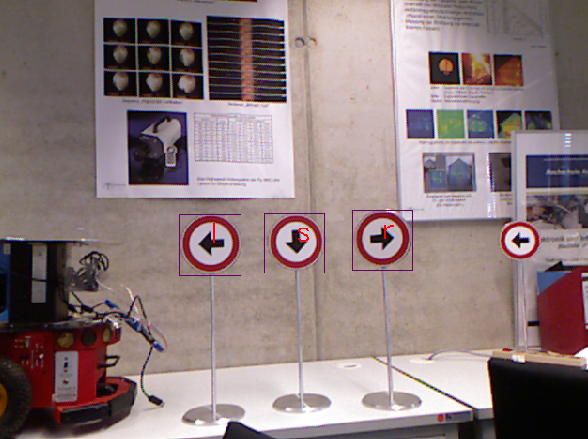
\includegraphics[width=\textwidth]{three.png}
  \caption[All Three Signs Matched]{All Three Signs Matched\footnotemark}
  \label{figure:three}
\end{center}
\end{figure}
\footnotetext{Sign on the right is not inside the current maximum distance}

\chapter{Conclusion}
\graphicspath{{./Conclusion/img/}}

The current procedure often doesn't find a sign in many frames, the reason for that is the very high congruence and coverage
treshhold. When decreasing it, the signs are found more often, but there are also many false positives. False positives are
even worse than only finding a surface once in 100 frames. When a robot drives along a track or just 
straight forward in the direction of a sign. There are many different viewing angles and a lot of frames will pass the algorithm,
till it reaches a point, where it can't see the sign, there are a lot of chances to get a positive and true match. But if
using a lower minimum for the congruence a lot of false positives may occur, so a method has to be found to find out
which one is a true and which one a false result if gathering multiple different matches for a surface.
Unfortunately, in many cases there are a lot of false positives when allowing a congruence smaller than 87\%, so 
it will be impossible to obtain the right match for a sign with only analyzing the amount of finds.
A good possiblity would be, to track the object and then get the best match while seeing the object.
But unfortunately there was not enough time to implement such a piece of software in the end. 
Table \vref{table:RESULT} shows the settings which have proven to be suitable for each processing step.

\begin{table}[H]
	\centering
	\begin{tabular}{lcc}
		Process Step Setting 							   & Value                 & Unit \\
		Bluring Depth Map Size							   & 5\footnotemark[1]     & px   \\
		Bluring Angle Map Size							   & 16\footnotemark[1]    & px   \\
		Angle Filter (Z-Axis Min-Max)                      & 10-35                 & degrees \\
		Surface Width (Min-Max)                            & 20-200                & px \\
		Surface Height (Min-Max)                           & 20-200                & px \\
		Template Matching Congruence (Min)                 & 87                    & percent \\
		Template Matching Coverage (Min)                   & 70                    & percent \\
	\end{tabular}
\caption{Software Setting Results}
\label{table:RESULT}
\end{table}
\footnotetext[1]{Distance from the center pixel}

The most interesting aspect of this work, is the invention of the neighborhood map. The neighborhood map has been proven
to be a good ally in bluring and seperating surfaces from a depth image. There where no performance
measures for a comparison of the bilateral filter delivered by OpenCV and the bluring method in this work,
but when using the bilateral filter to blur the depth image, a instant drop in the frame rate of the depth image is visible
without measuring it, when using the cross blur filter mentioned here, this isn't the case. Currently the only lack
of the neighboorhood map are edges, which aren't created by a object infront of a background, like marked in figure \vref{figure:InnerEdges}.
The reason for the missing feature is that it wasn't necessary, because only surfaces which look directly to the camera 
are interesting for sign recognition. For adding this feature a closer look at a gradient analysis of the depth image,
like it was done by Mr. Kühner in his bachelor thesis \cite{max:recog}, would be necessary,.

\begin{figure}[H]
\begin{center}
  \includegraphics[width=\textwidth]{innerEdge.png}
  \caption{Inner-Object-Edges (marked green)}
  \label{figure:InnerEdges}
\end{center}
\end{figure}

Another interesting aspect is the template matching algorithm, which searches for proportions and resizes the
template to the appropriate size. The advantage of this algorithm is clearly that a image has to be passed
only once for finding suitable proportions and the template will be scaled properly, making it possible
to find matches in a huge range of different scalings. In a normal template matching algorithm,
this would mean to shift a template all over the picture and compare it at any place, taking a lot
of time for processing. A disadvantage of this template matching functionality is that it will not
find the template inside of a picture when the surface is rotated, but in this work, this is
is done by using the real world coordinates to warp the perspective, so the target pattern
will be visible at the right proportions. But unfortunately there's another disadvantage,
if the camera is rotated a few degrees, the alogrithm will not find the picture anymore.
A approach to this problem could be to try to read out the accelerometer of the Kinect,
to rotate the image according to the gravity direction.

Now to the real goal of the work, using the depth image data for only searching in suitable surfaces,
which are filtered by their size and der angle to the camera. Filtering out these surfaces
is really a good idea, because it decreases the picture area where a sign has to be searched.
When allowing the areas to be really small or big, the frame rate drops dramatically. Also
the angle filtering is doing it's part to minimize the prospect and to increase the performance
of the software.

\nocite{willowgarage:rostutorials}


\bibliographystyle{babplain}
\bibliography{mybib}
\end{document}  